\subsection{Дискретный анализ}
	
	\subsubsection{Аннотация}

	    Курс <<Дискретный анализ>> получил смешанные отзывы. 
        
        Респонденты отметили, что лекции Ильинского Д.Г. зачастую были непонятны из-за плохого почерка и дикции лектора. Совет студентов и аспирантов ФРКТ просит передать эти сведения лектору.

        Семинарист Табунов А.В. получил крайне положительные оценки от респондентов. Совет студентов и аспирантов ФРКТ предлагает поощрить этого преподавателя.

        Руководствуясь результатами опроса, Совет студентов и аспирантов ФРКТ выдвигает следующие идеи по улучшению данного курса:
        \begin{enumerate}
            \item сделать курс, ориентированным на программирование, т.е. разбирать, как дискретный анализ применяется в различных алгоритмах.
        \end{enumerate}


	\subsubsection{Общий отзыв студентов о курсе}

		\begin{figure}[H]
			\centering
			\begin{subfigure}[b]{0.45\textwidth}
				\centering
				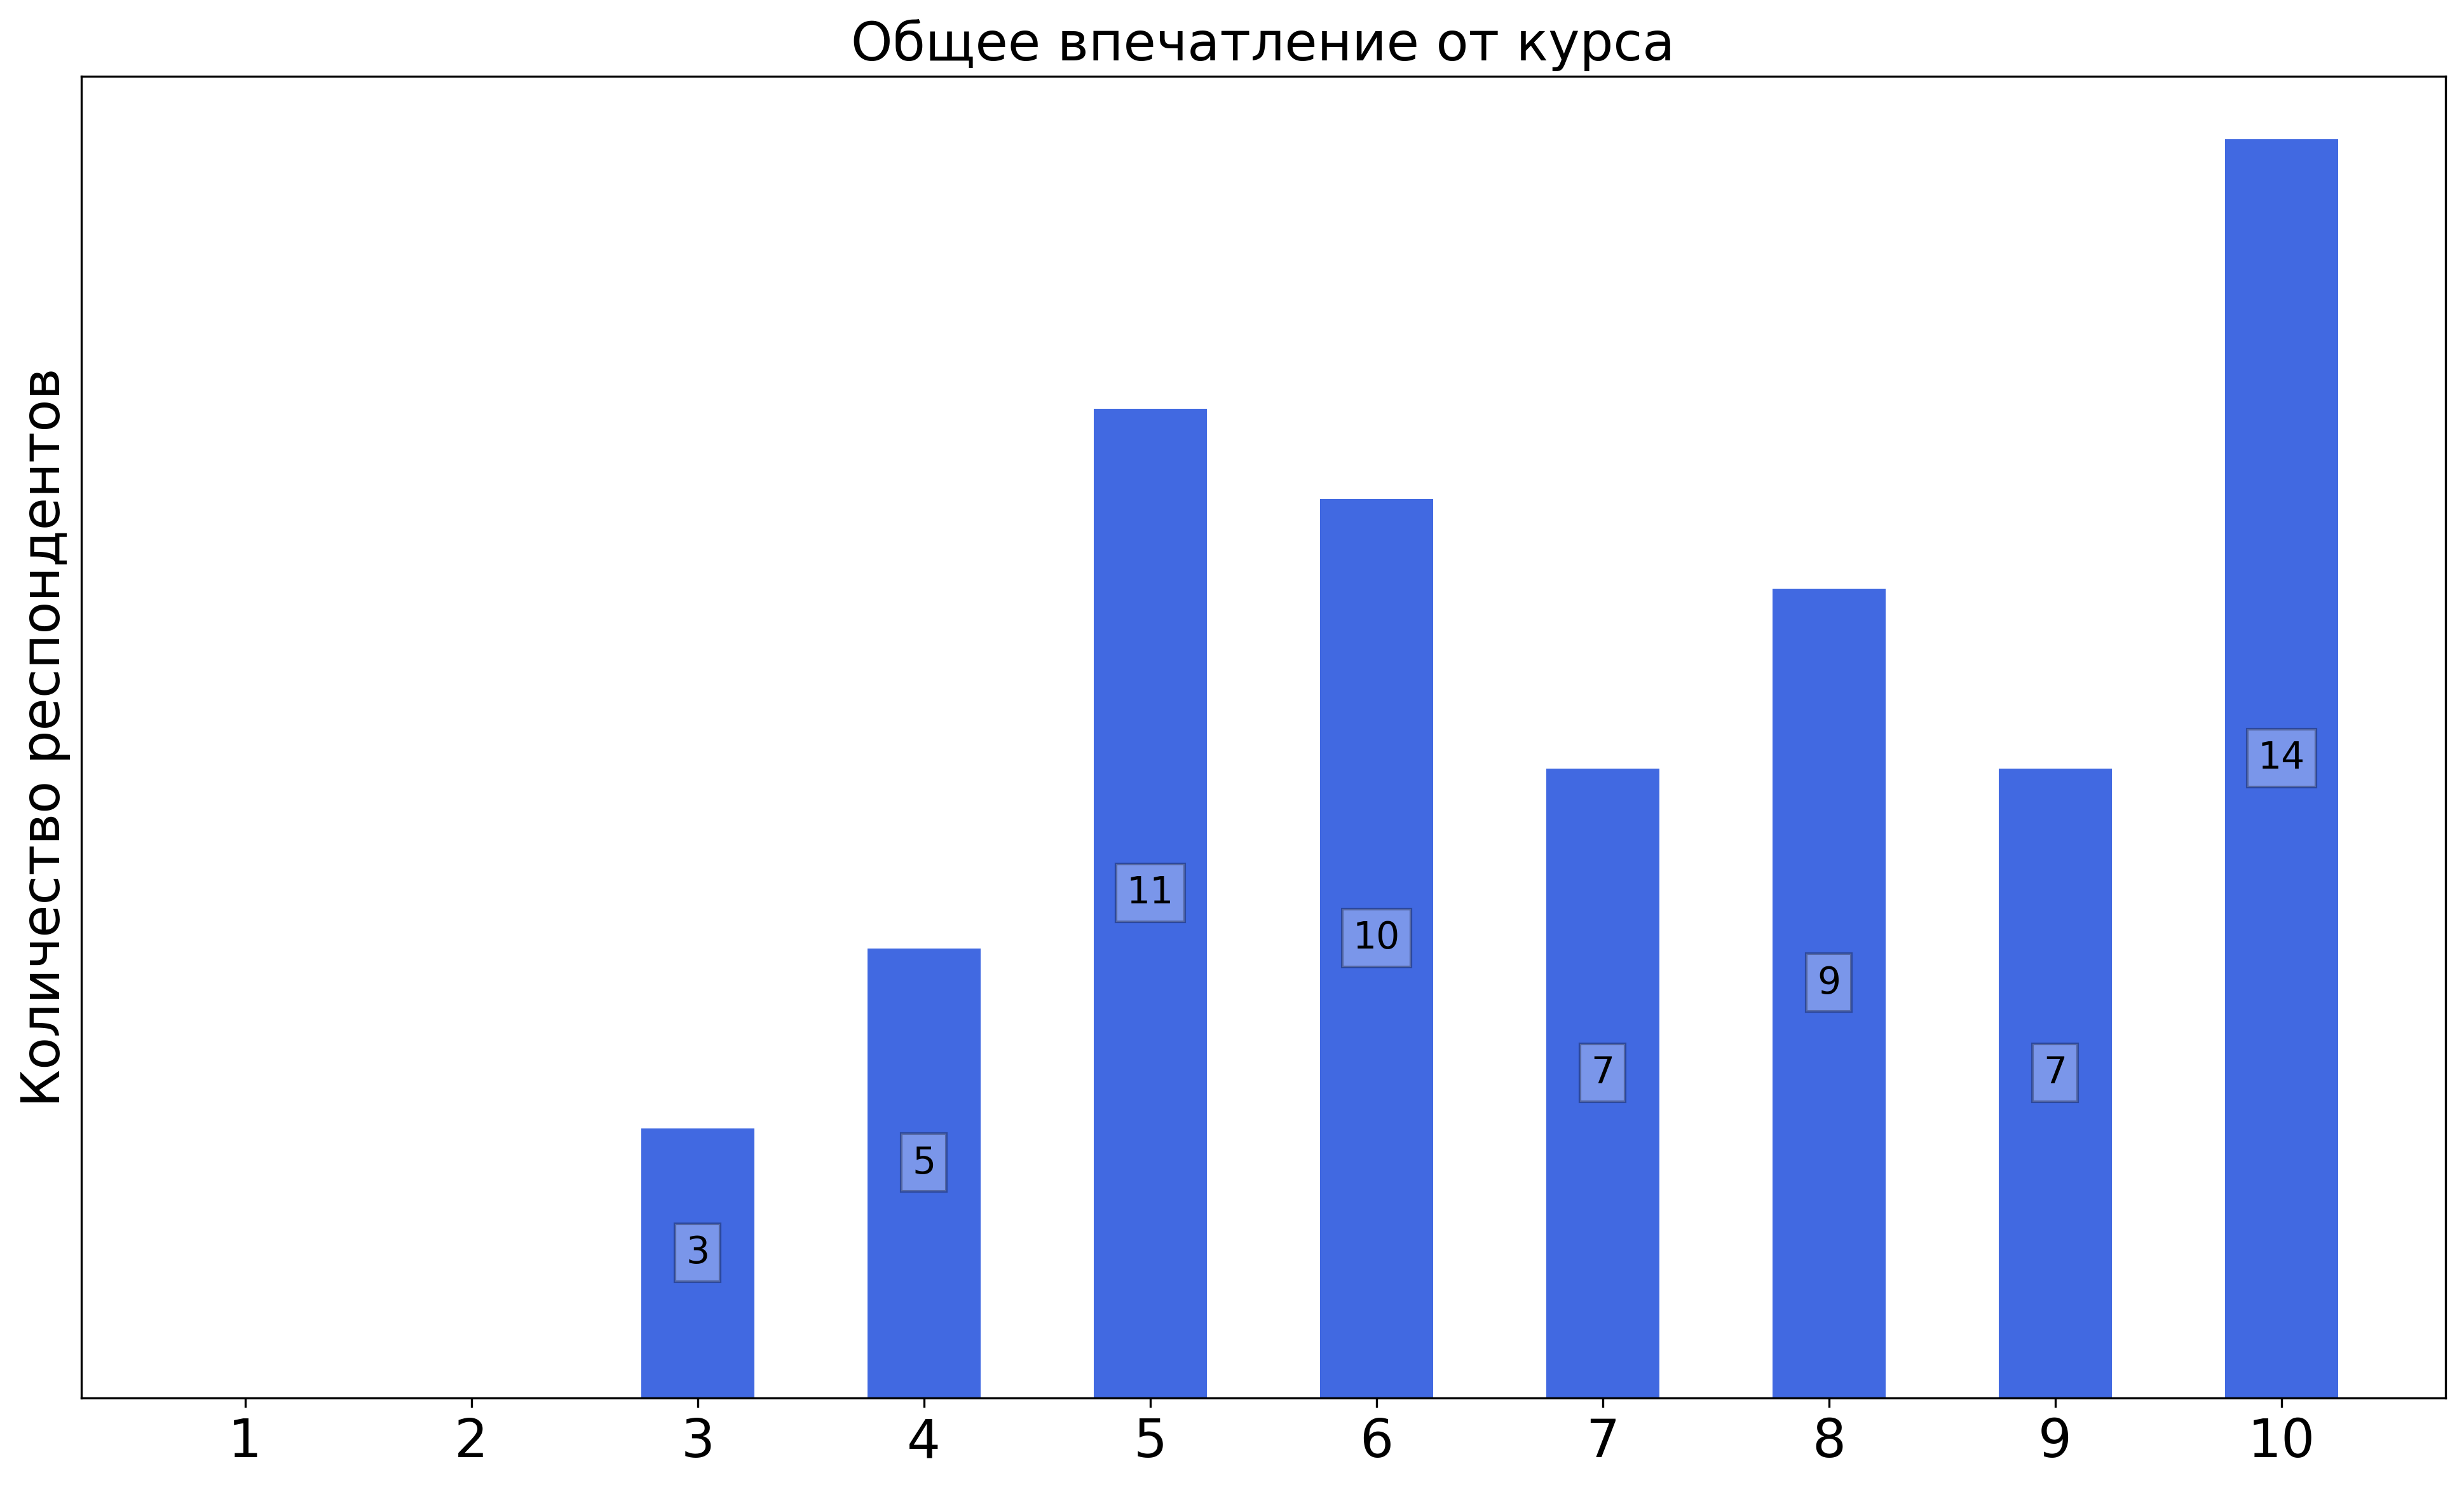
\includegraphics[width=\textwidth]{images/1 course/Дискретный анализ/general-0.png}
			\end{subfigure}
		\end{figure}

	\subsubsection{Материалы, использумые респондентами при изучении курса}

		\begin{figure}[H]
			\centering
			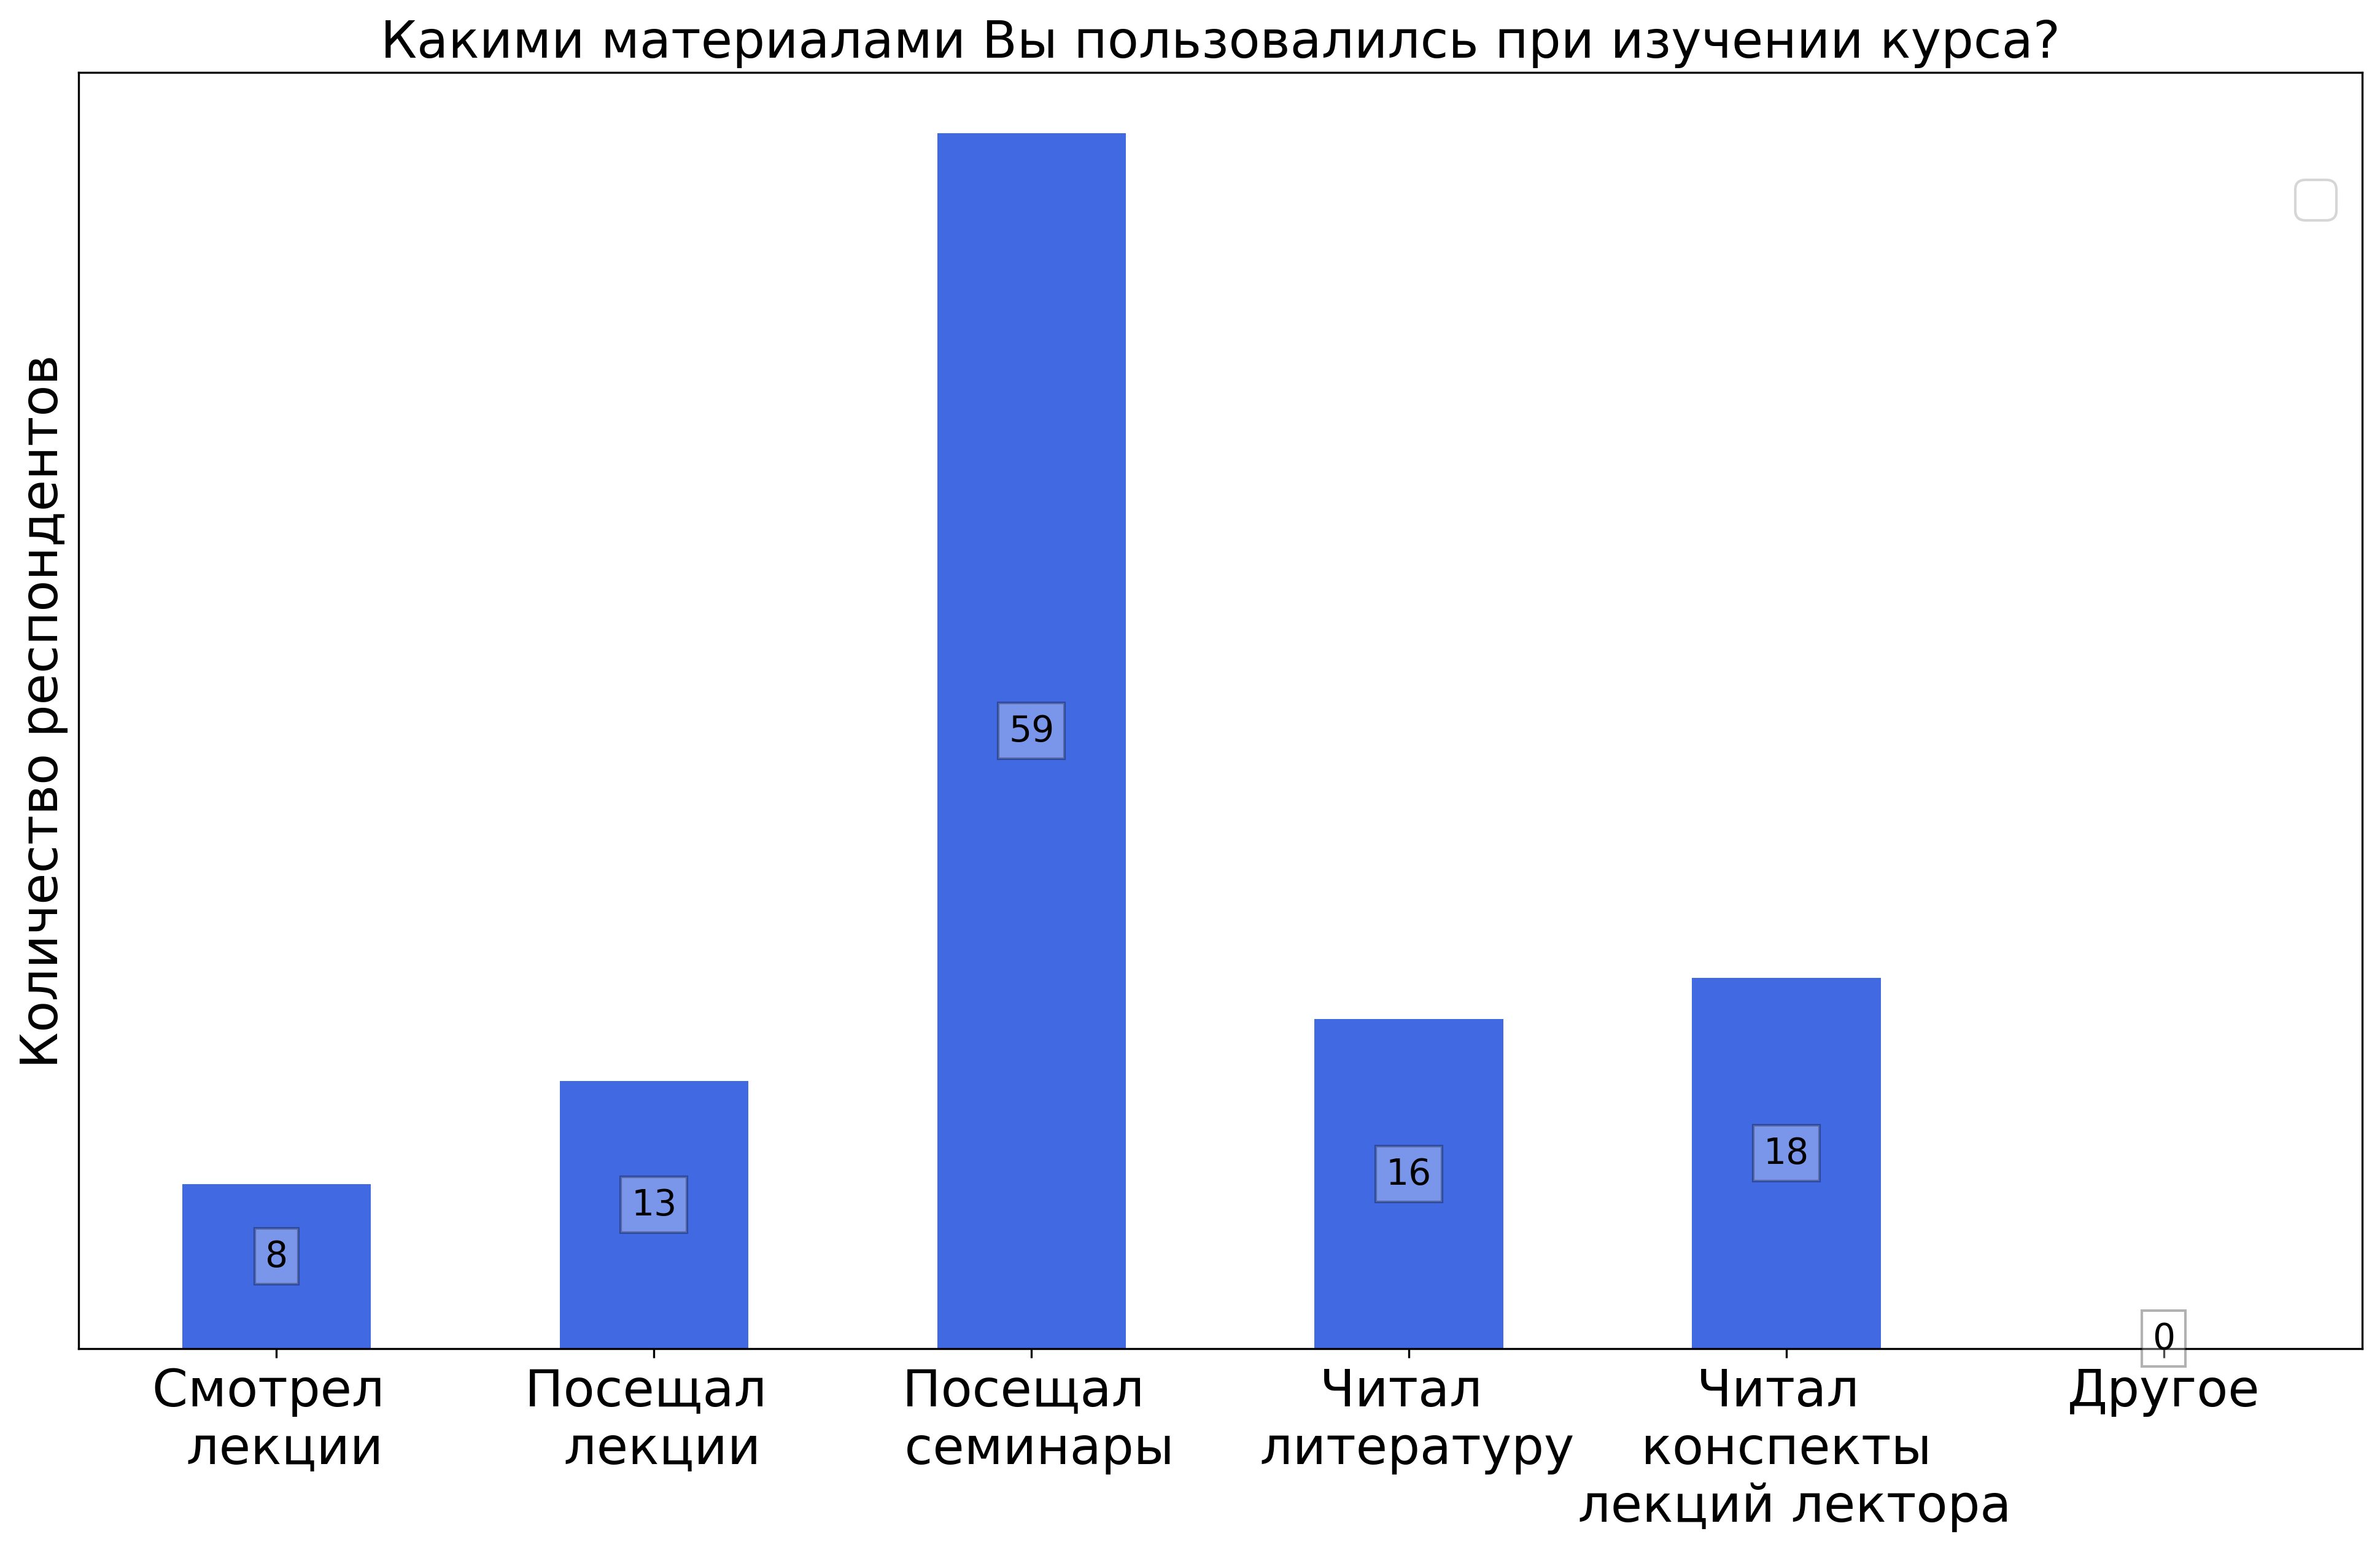
\includegraphics[width = 0.45\textwidth]{images/1 course/Дискретный анализ/materials.png}
		\end{figure}

	\subsubsection{Отзыв студентов о лекциях. Лектор: Ильинский Д.Г..}

		\begin{figure}[H]
			\centering
            \begin{subfigure}[b]{0.45\textwidth}
				\centering
				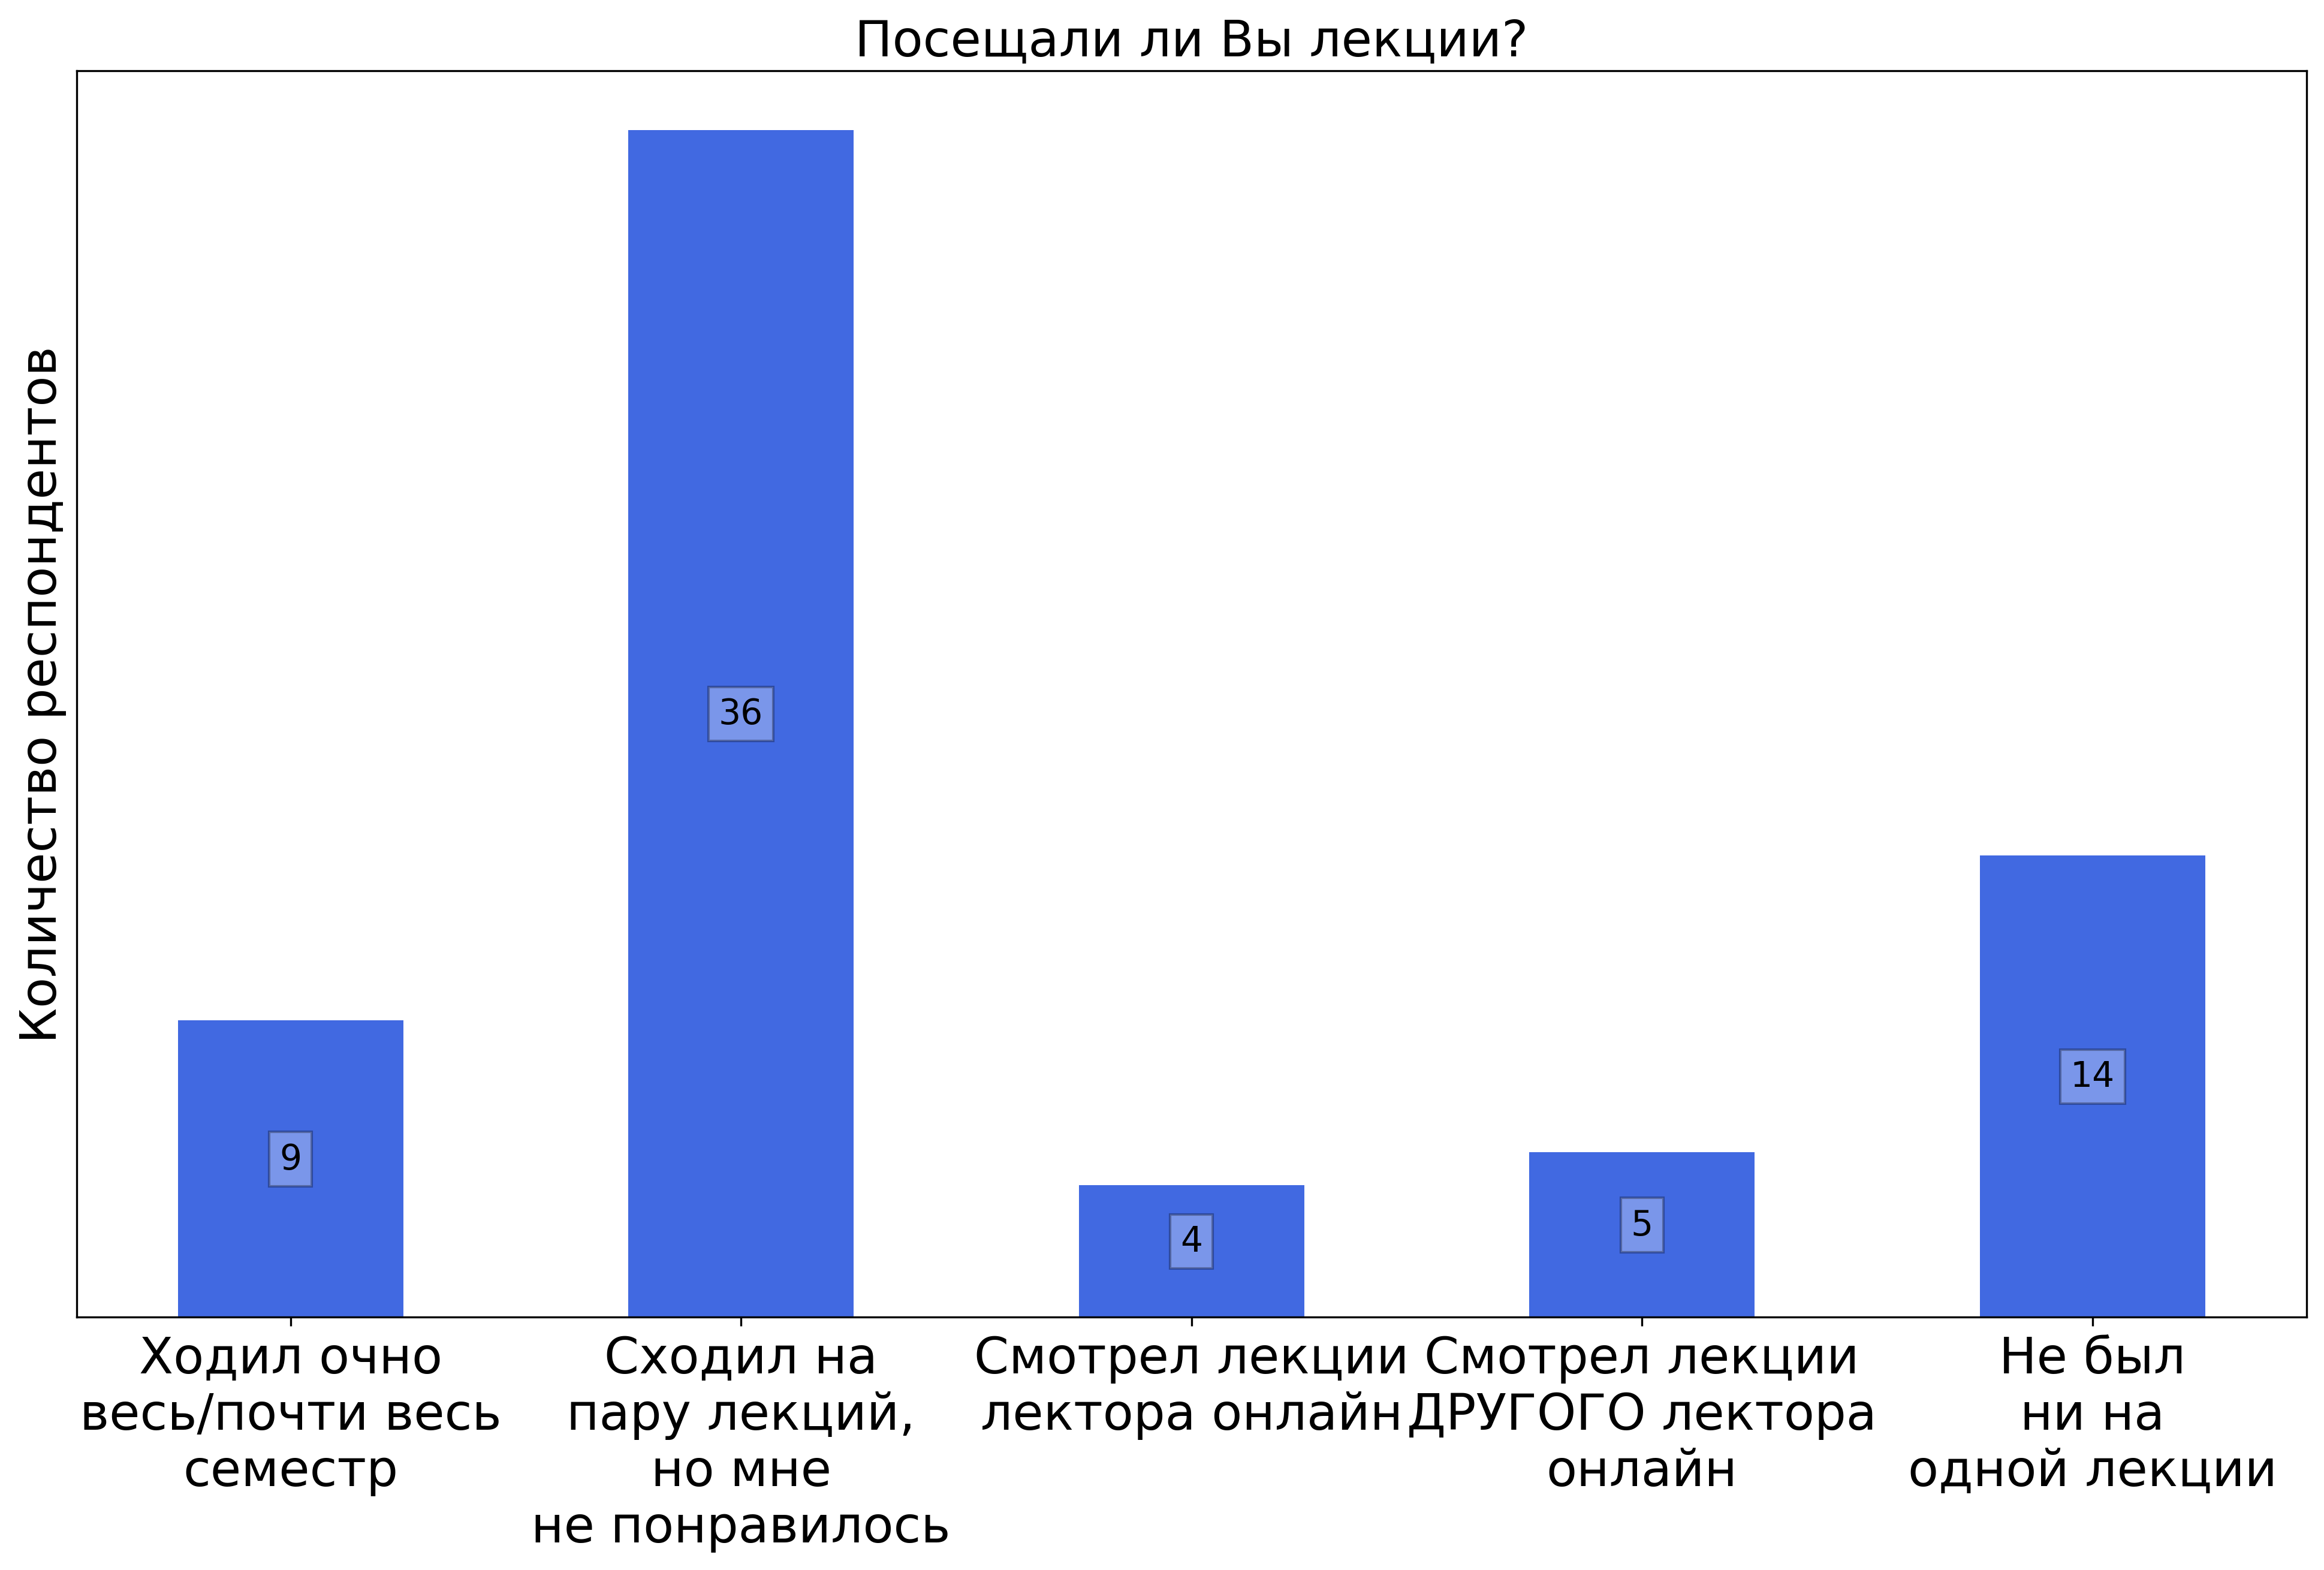
\includegraphics[width=\textwidth]{images/1 course/Дискретный анализ/lecturer-questions-Ильинский Д.Г.-0.png}
			\end{subfigure}
			\begin{subfigure}[b]{0.45\textwidth}
				\centering
				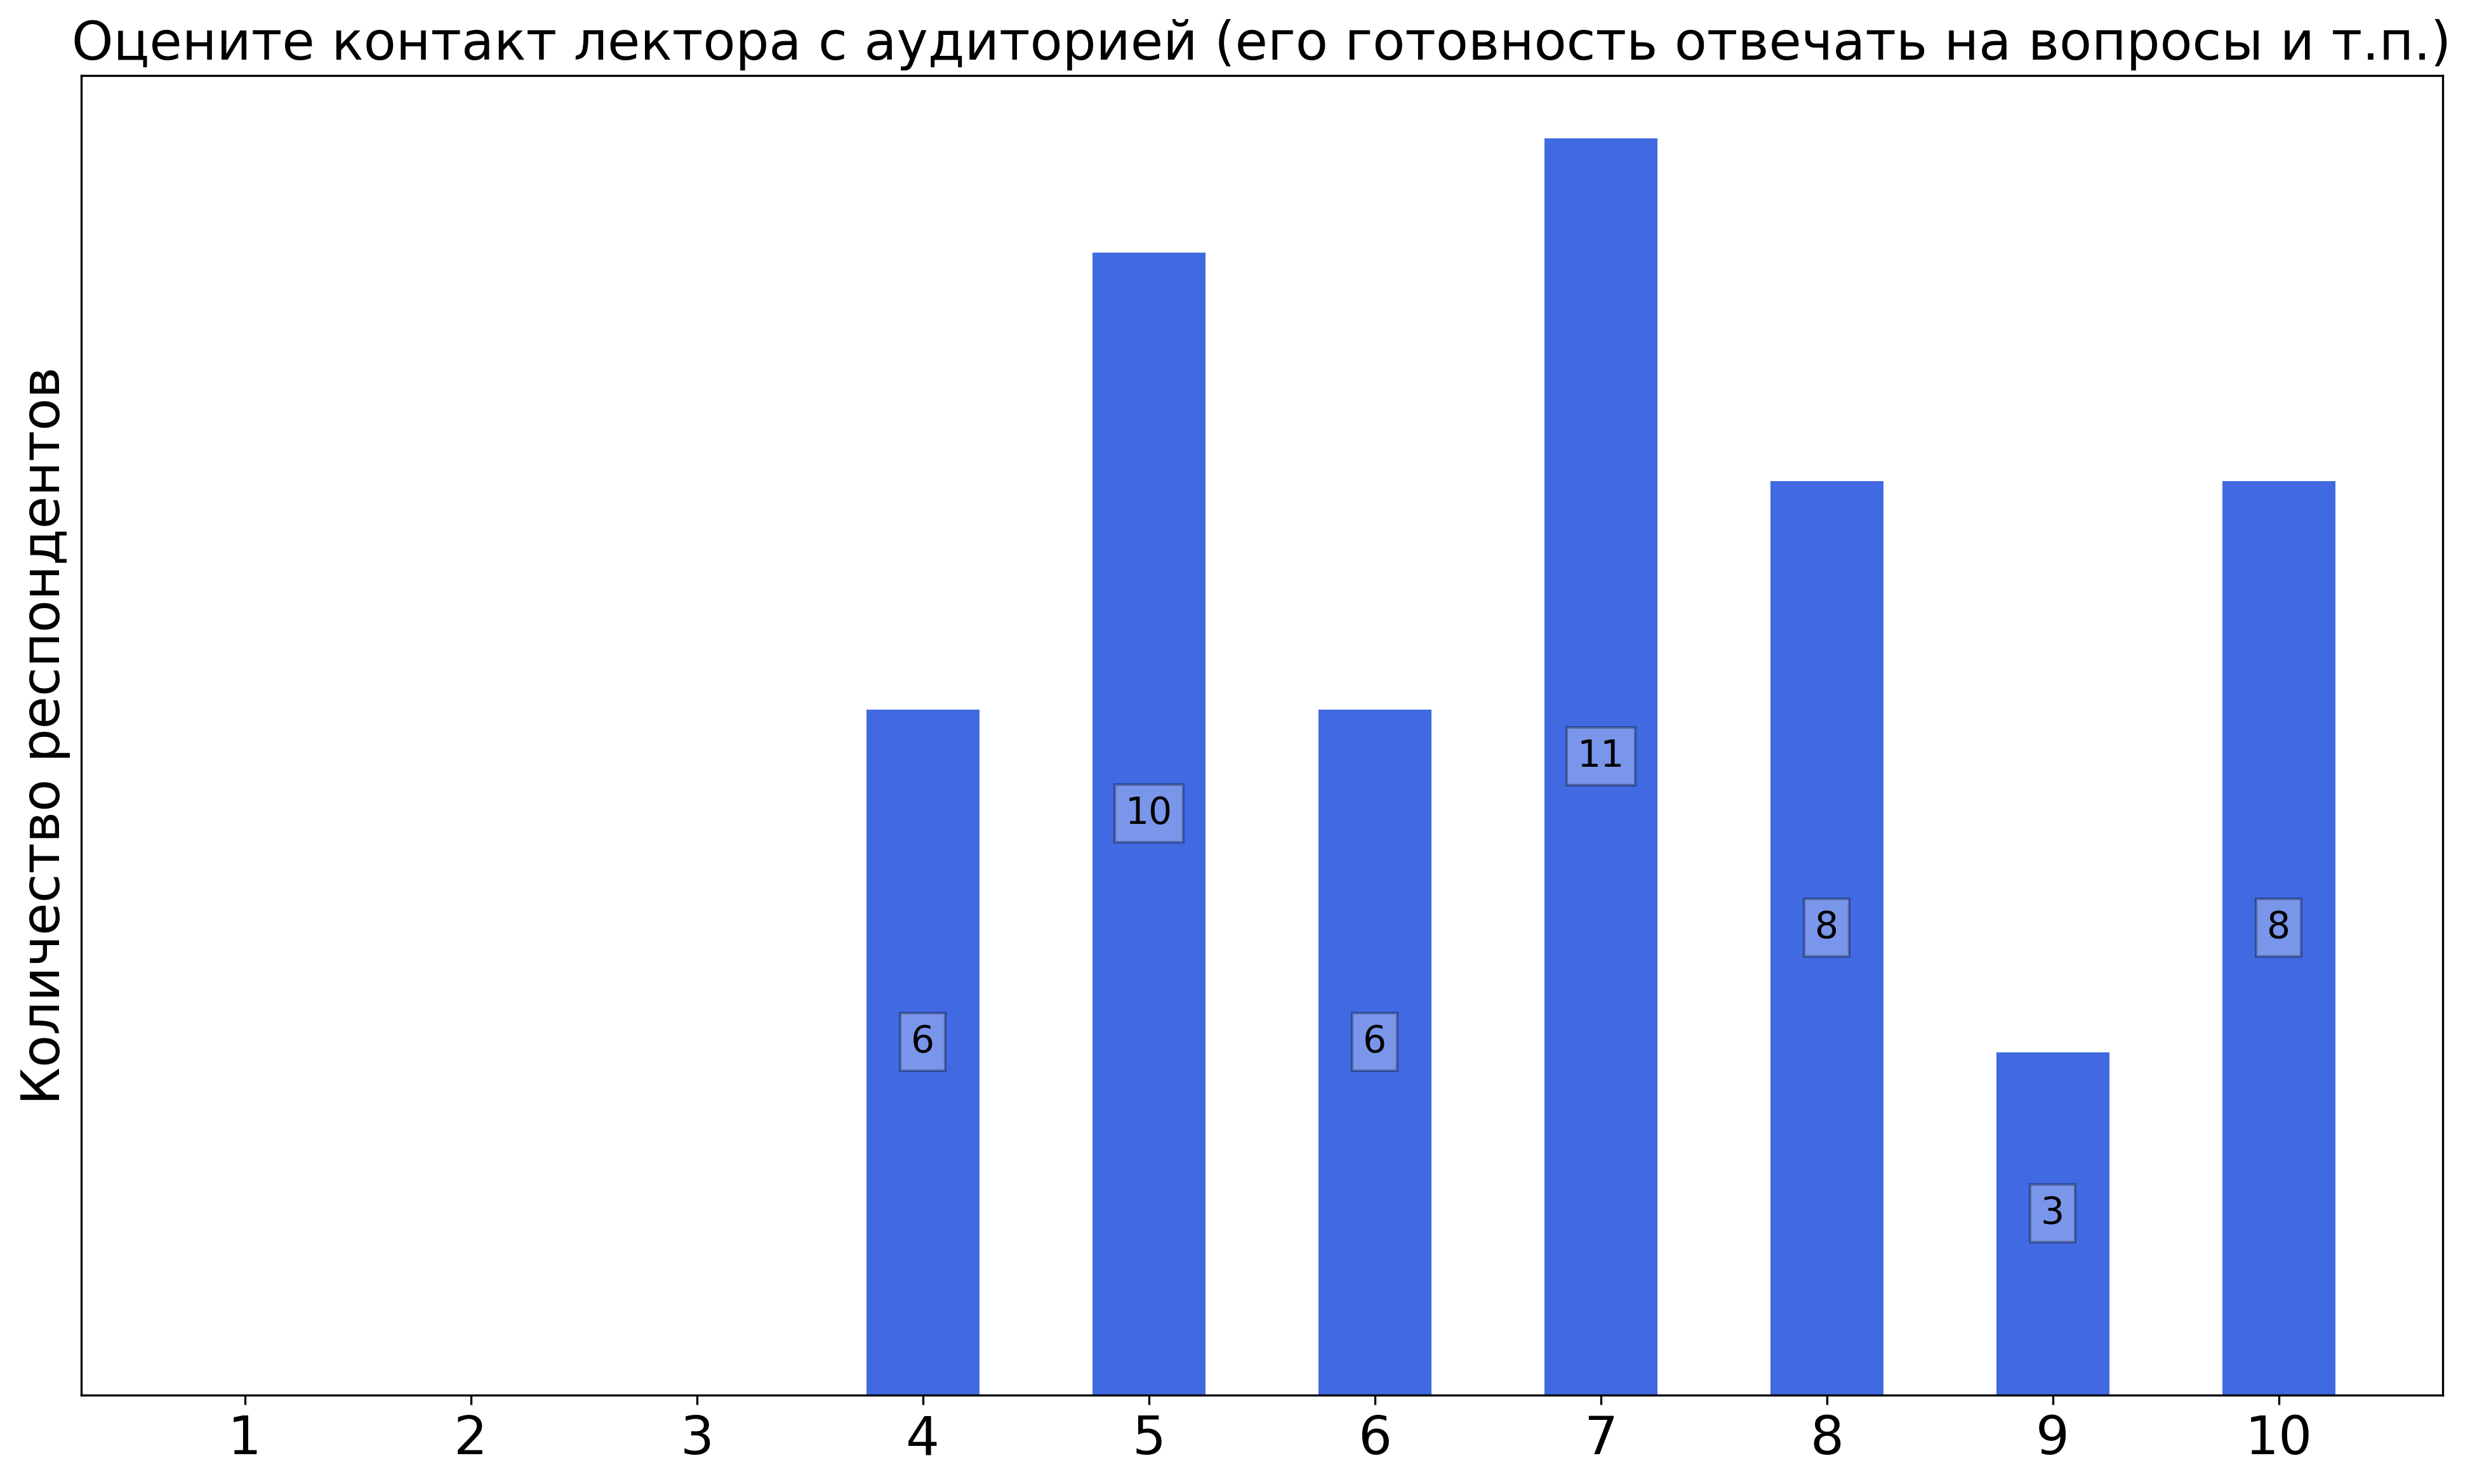
\includegraphics[width=\textwidth]{images/1 course/Дискретный анализ/lecturer-marks-Ильинский Д.Г.-0.png}
			\end{subfigure}
			\begin{subfigure}[b]{0.45\textwidth}
				\centering
				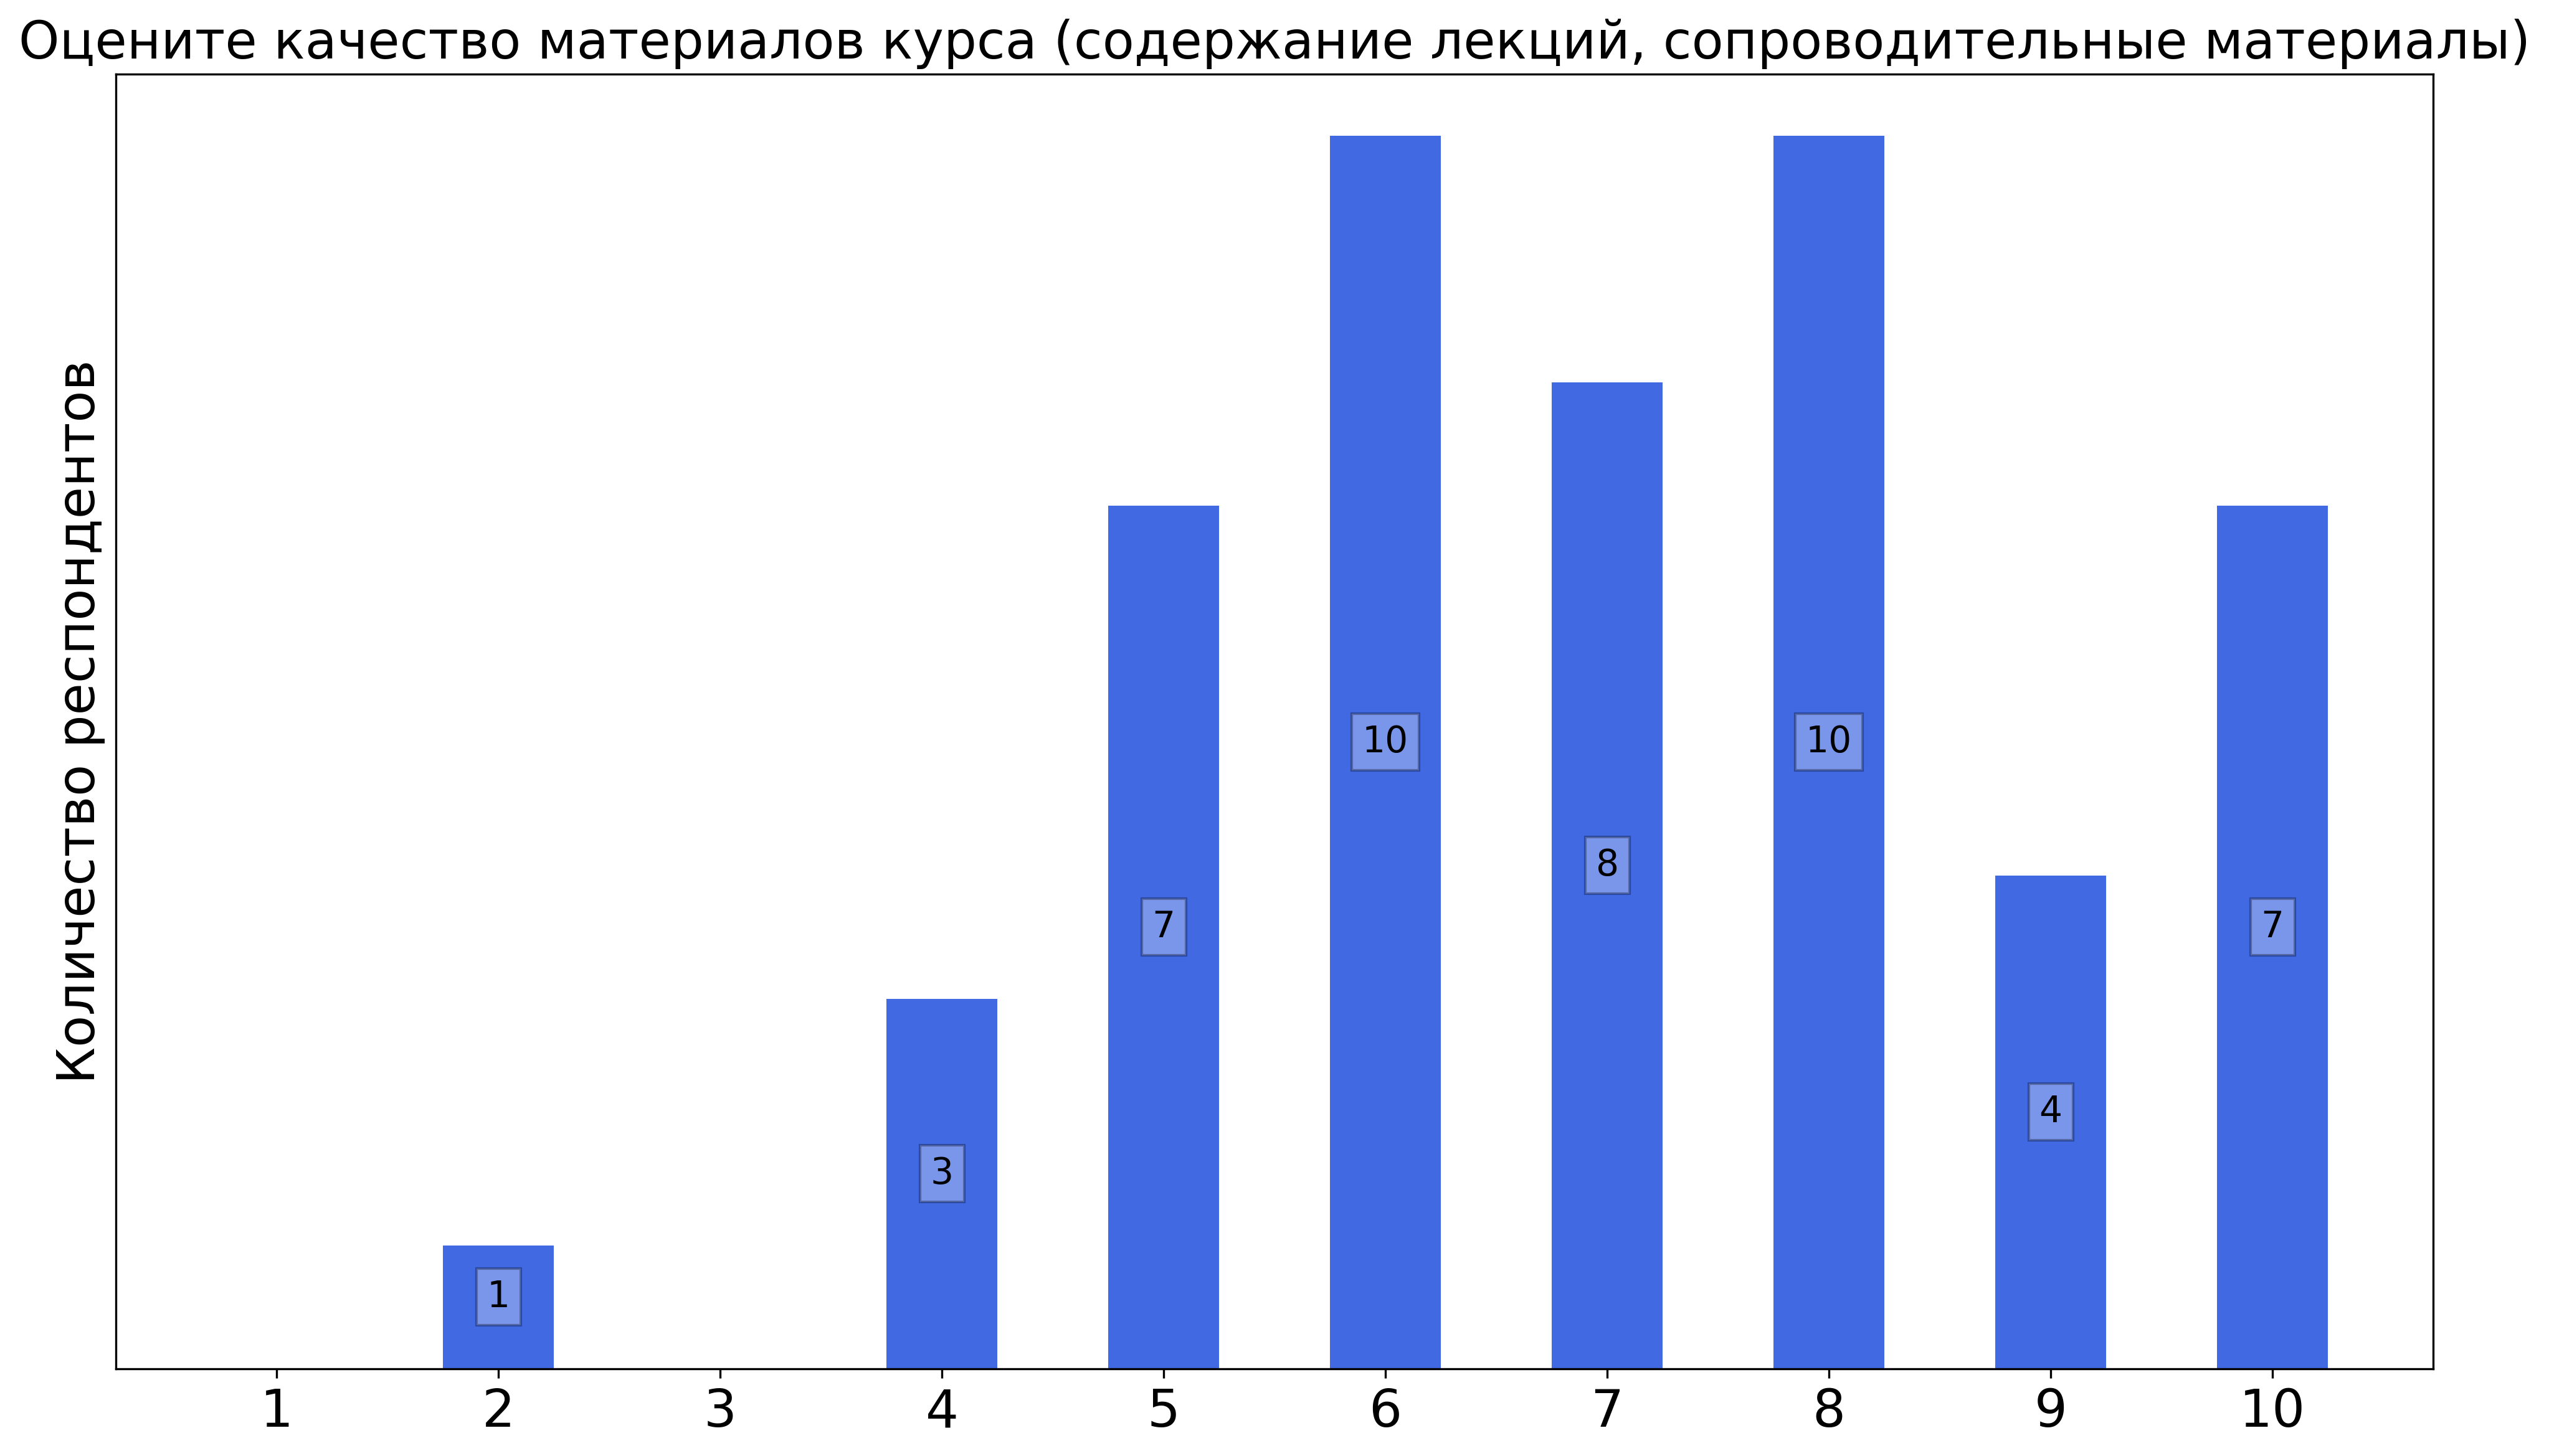
\includegraphics[width=\textwidth]{images/1 course/Дискретный анализ/lecturer-marks-Ильинский Д.Г.-1.png}
			\end{subfigure}
			\begin{subfigure}[b]{0.45\textwidth}
				\centering
				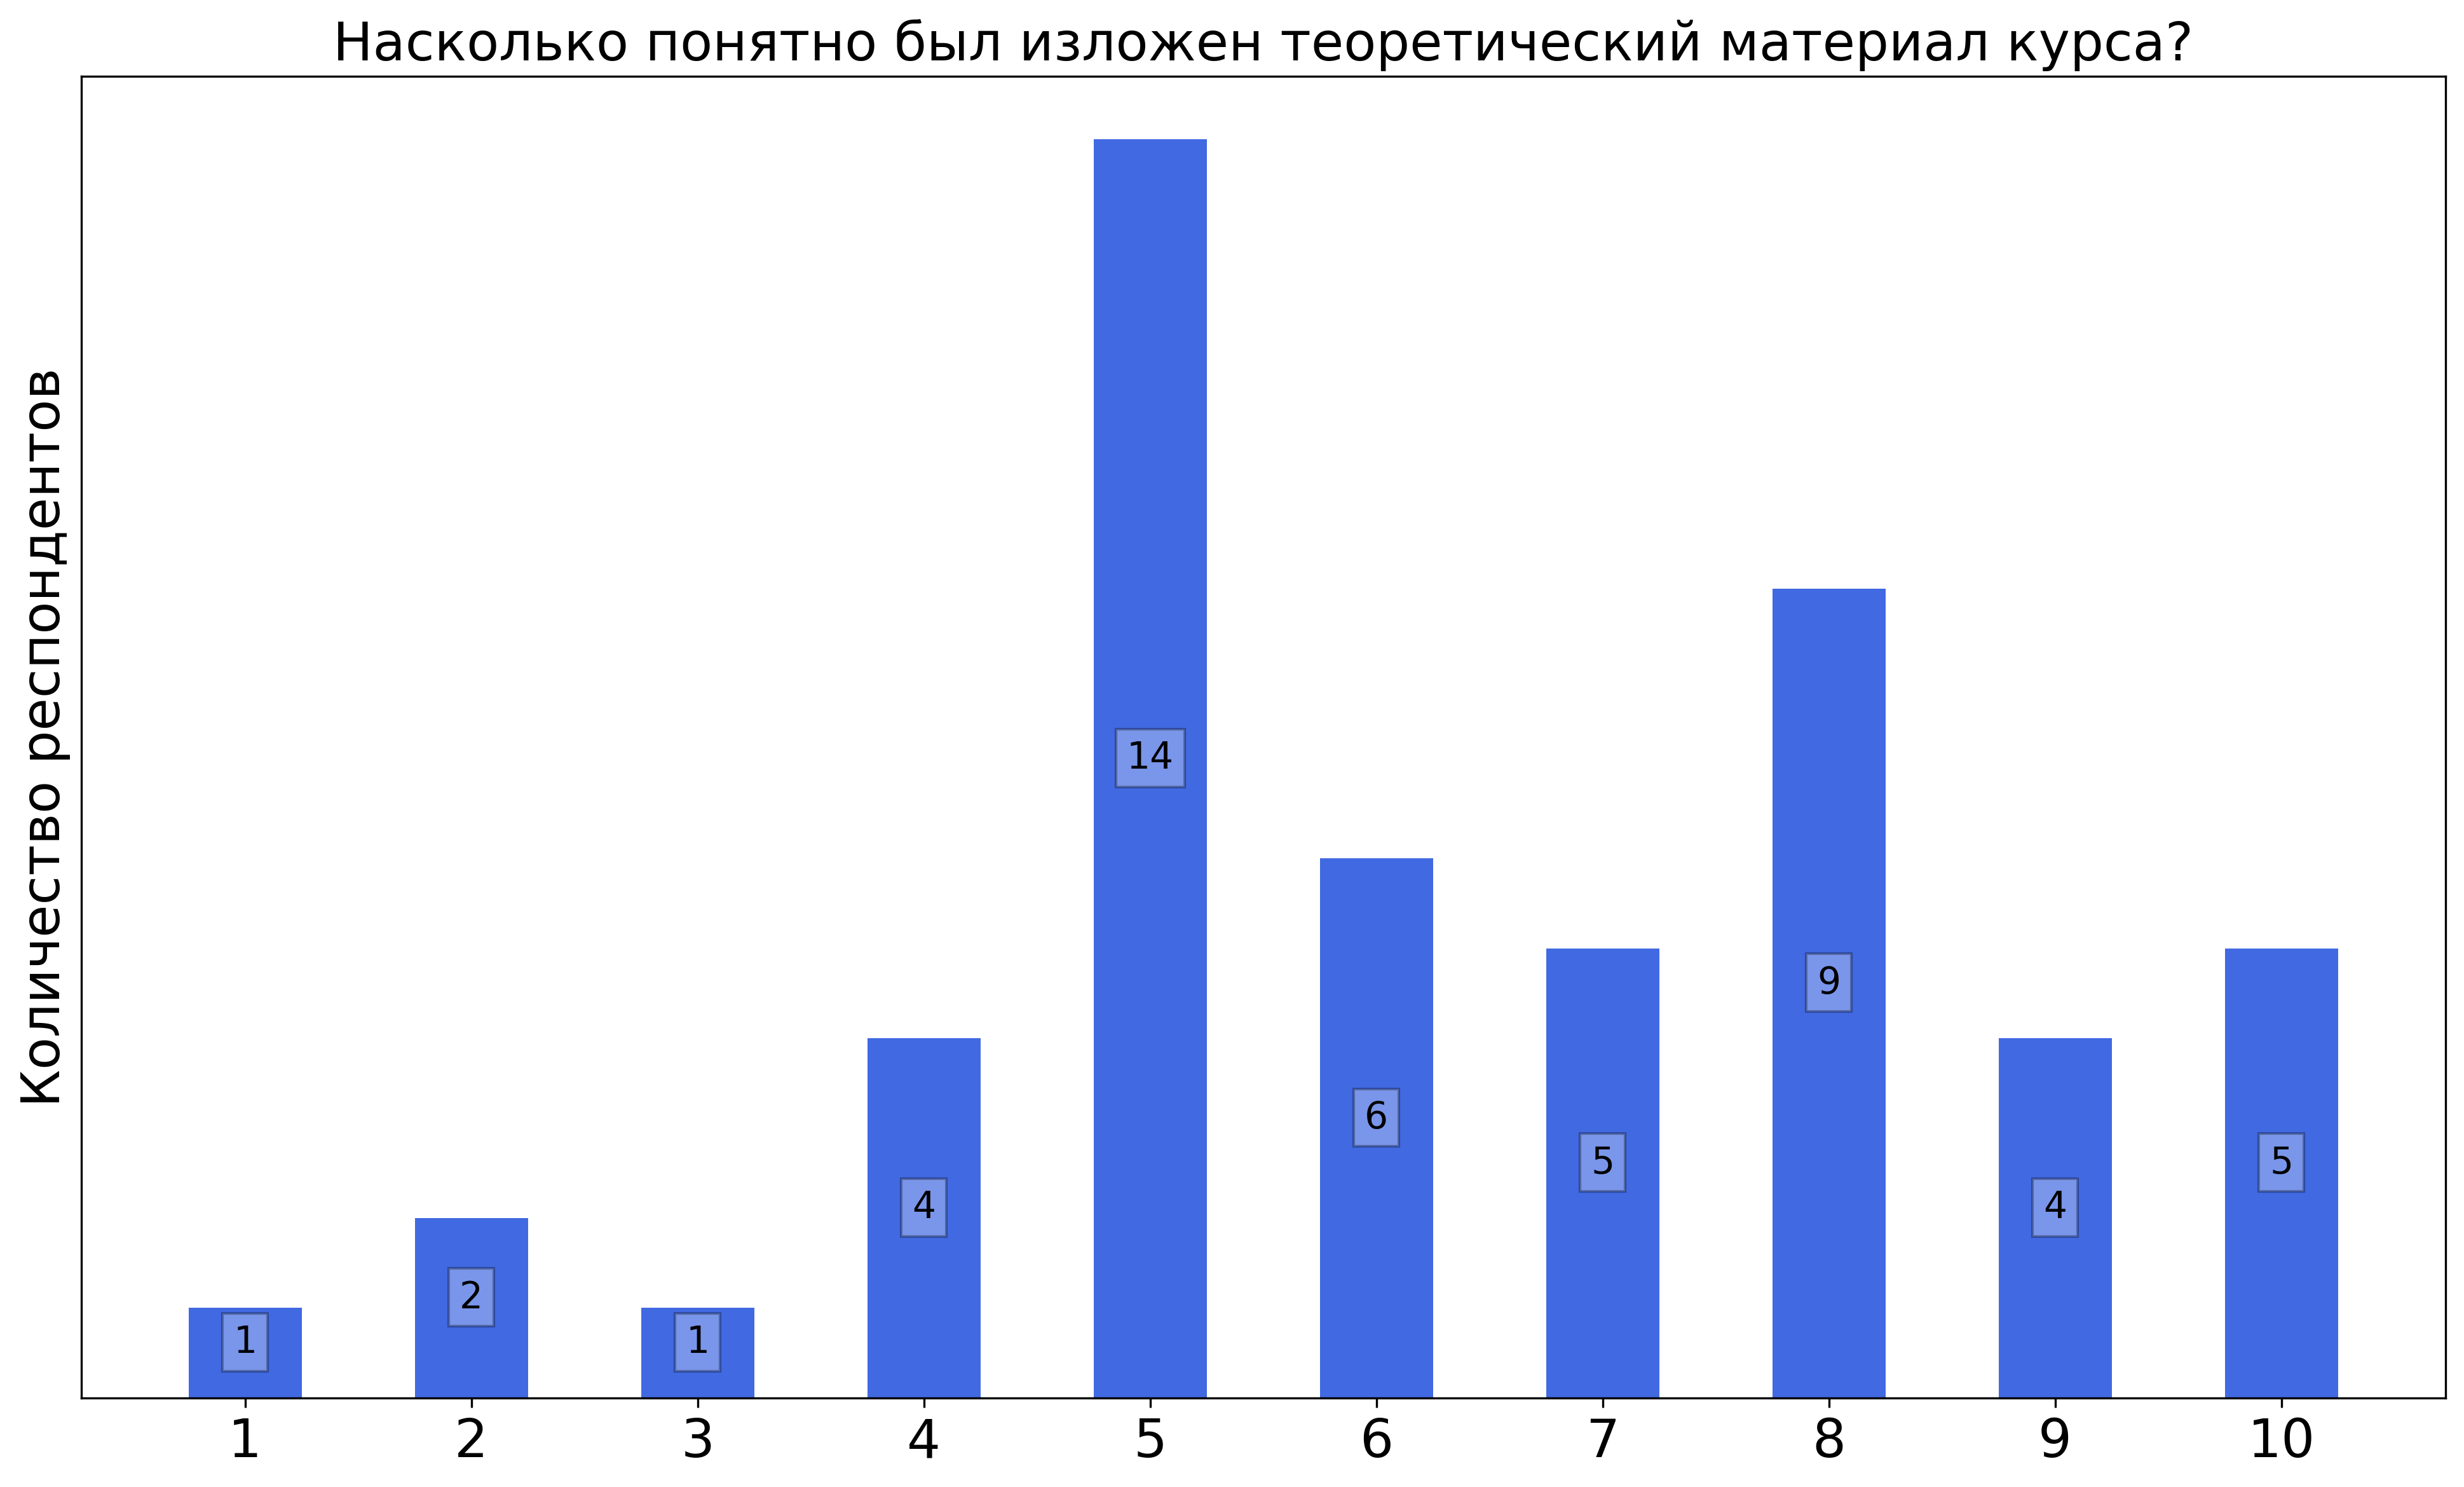
\includegraphics[width=\textwidth]{images/1 course/Дискретный анализ/lecturer-marks-Ильинский Д.Г.-2.png}
			\end{subfigure}	
			\begin{subfigure}[b]{0.45\textwidth}
				\centering
				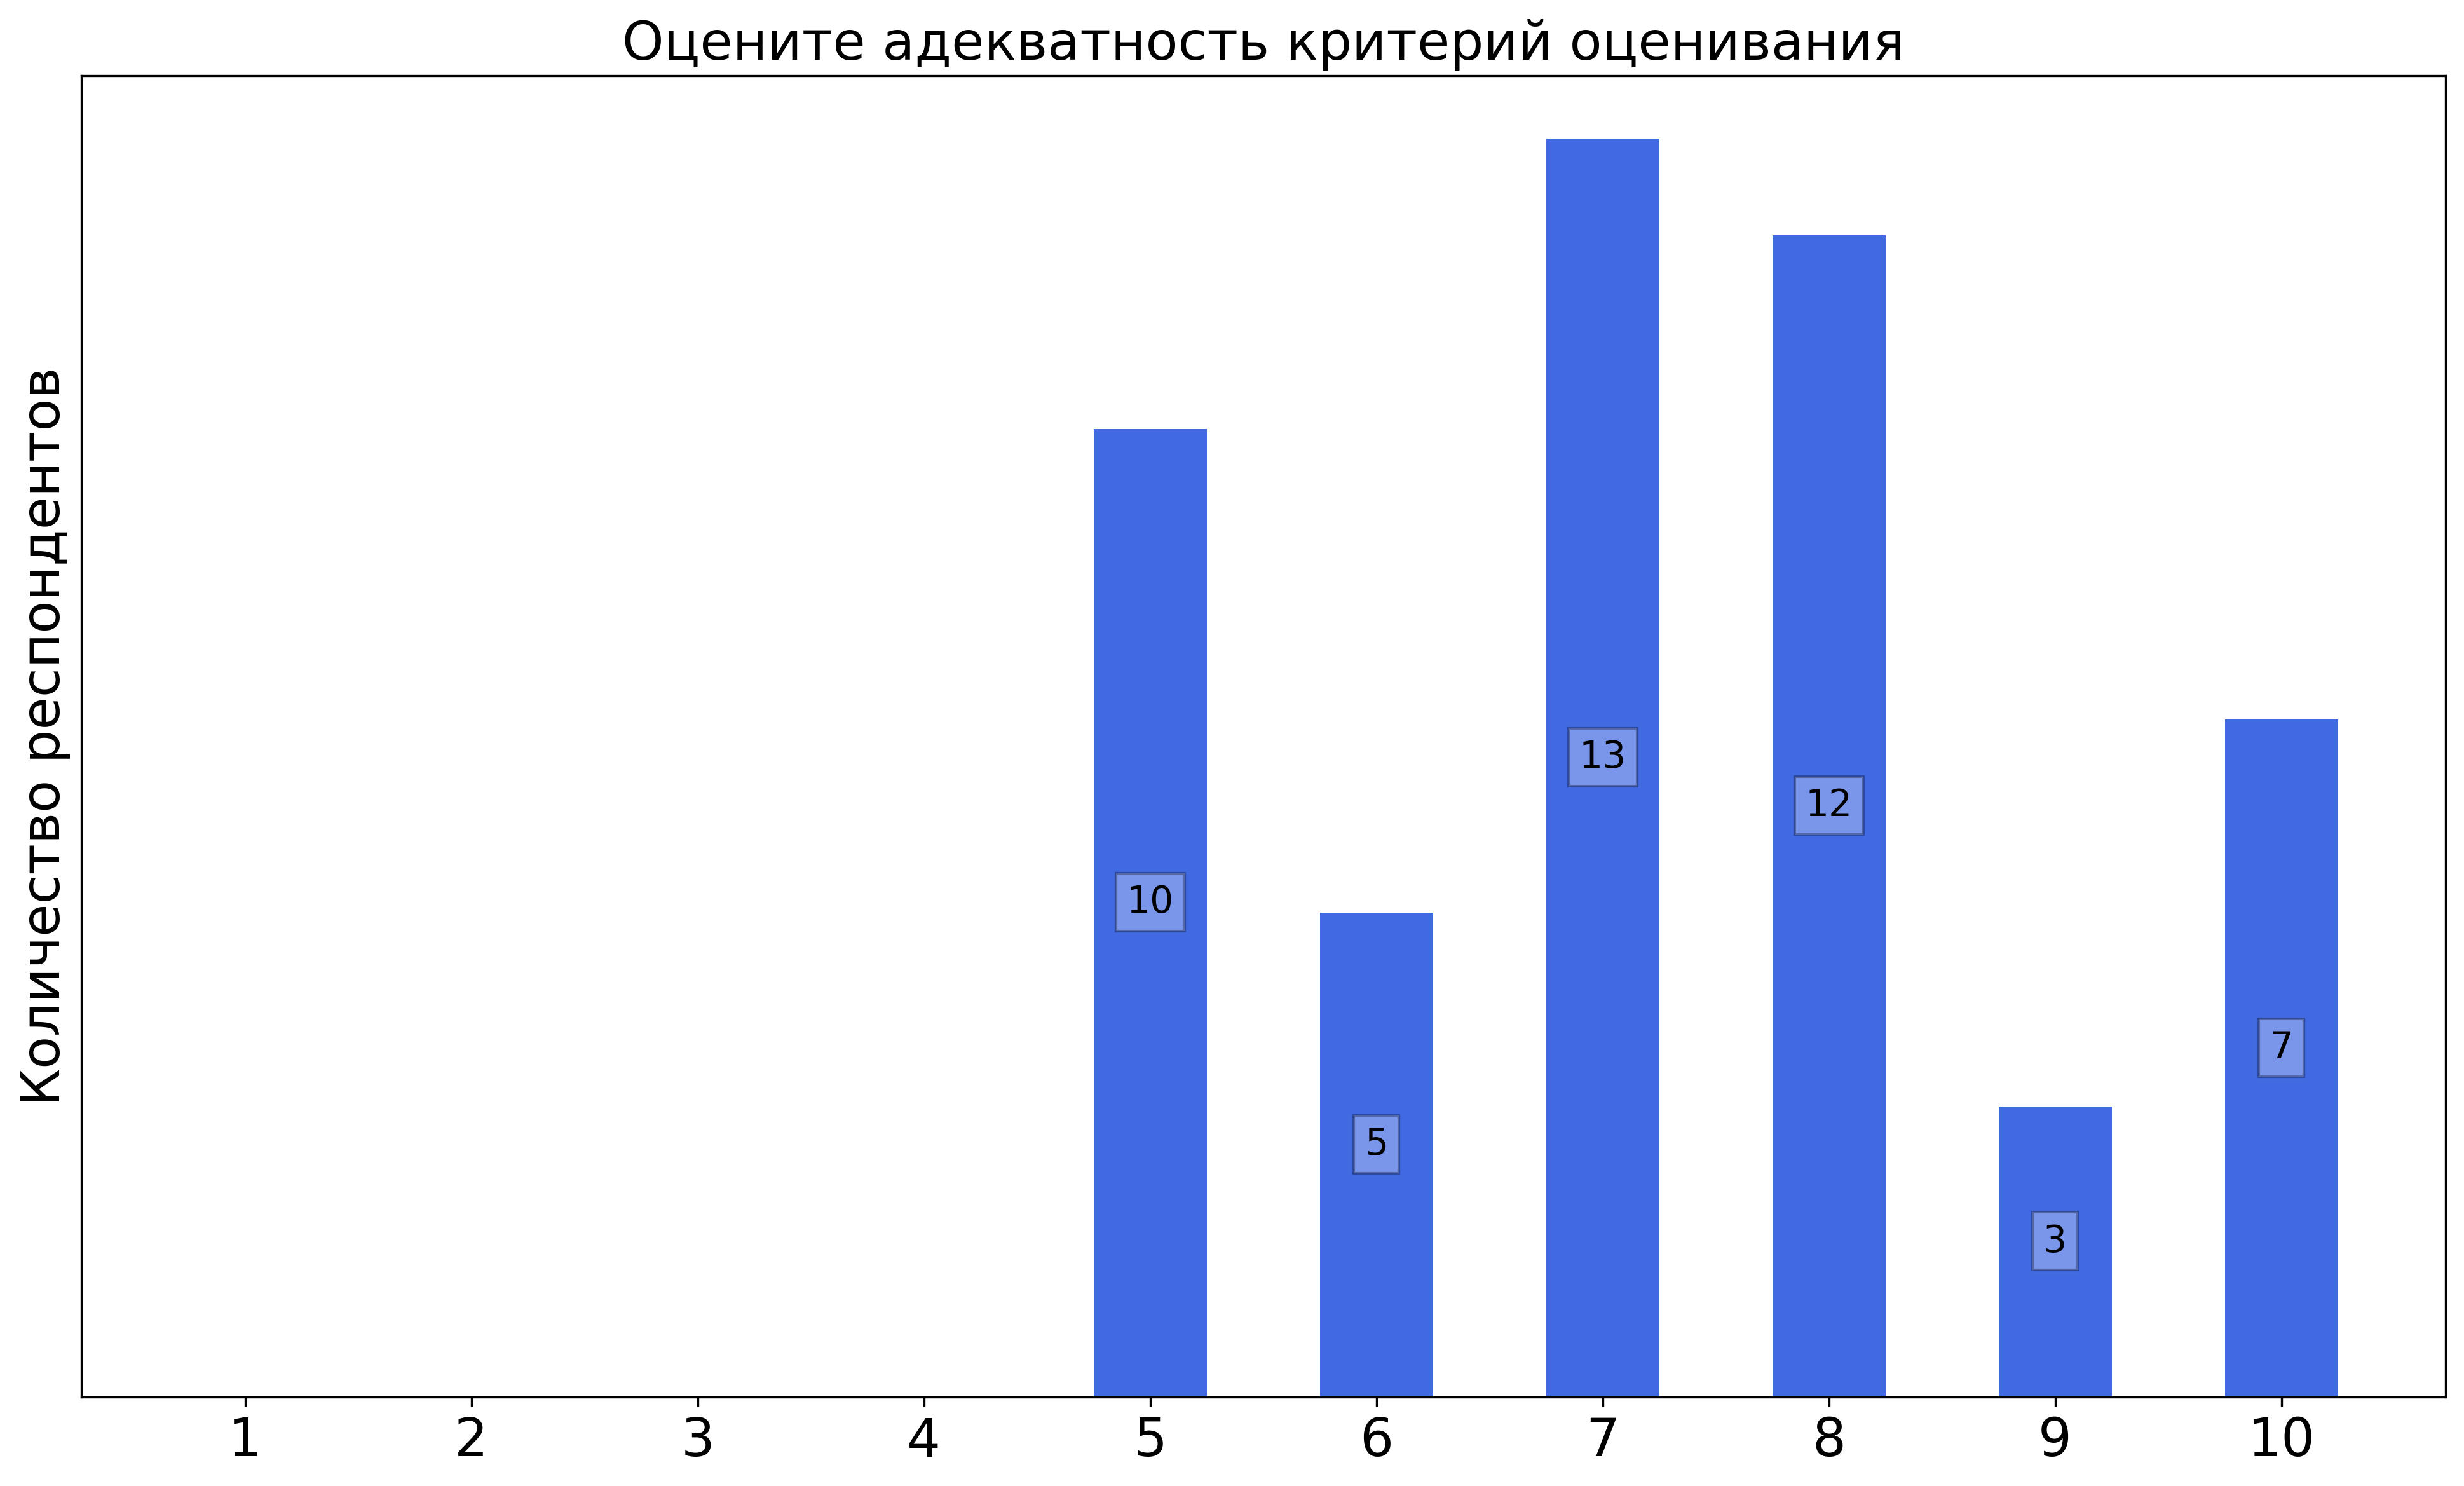
\includegraphics[width=\textwidth]{images/1 course/Дискретный анализ/lecturer-marks-Ильинский Д.Г.-3.png}
			\end{subfigure}
			\caption{Оценки респондентов о качестве преподавания лекций по курсу <<Дискретный анализ>>}
		\end{figure}

		\textbf{Комментарии студентов о лекциях\protect\footnote{сохранены оригинальные орфография и пунктуация}}
            \begin{commentbox} 
                просто  легкий предмет, закрываемый без лекций 
            \end{commentbox} 
        
            \begin{commentbox} 
                Очень быстро, речь сливается, почерк просто на уровне (доктора даже лучше пишут) Смотрел Рубцова, ему благодарность огромная. 
            \end{commentbox} 
        
            \begin{commentbox} 
                Хз, поставлю отл ему, но я был на первых 3-х лекциях, а потом не ходил, т.к. на семинарах совсем другой курс был. Очень быстро читает лекции, поэтому не очень  
            \end{commentbox} 
        
            \begin{commentbox} 
                Очень быстро говорит, но если пытаться вникать и не отвлекаться, то можно все понять 
            \end{commentbox} 
        
            \begin{commentbox} 
                Дикция лектора затрудняет восприятие материала. Если бы замедлил темп речи (не темп лекции) раза в полтора - стало бы понятней. 
            \end{commentbox} 
        
            \begin{commentbox} 
                Очень быстро, но можно задавать вопросы. 
            \end{commentbox} 
        
            \begin{commentbox} 
                Очень сумбурно, быстро читались 
            \end{commentbox} 
        
            \begin{commentbox} 
                не шарю за лекции, ни на одной не был 
            \end{commentbox} 
        
            \begin{commentbox} 
                Не очень понятно объяснял. К тому же, программа не очень полезная, так как не совпадала с семинарами 
            \end{commentbox} 
        
            \begin{commentbox} 
                Очень быстрое изложение часто приводило к непониманию материала 
            \end{commentbox} 
        
            \begin{commentbox} 
                Слишком быстро говорил, не успеваешь записывать 
            \end{commentbox} 
        
            \begin{commentbox} 
                На лекции не было смысла ходить, потому что семинарист Бурцев. 
            \end{commentbox} 
        
            \begin{commentbox} 
                У нас был Бурцев, и его программа совсем отличалась от того, что происходило на лекциях 
            \end{commentbox} 
    
    
    \subsubsection{Отзыв студентов о семинарах. Семинарист: Бурцев А.А.}
		\begin{figure}[H]
			\centering
			\begin{subfigure}[b]{0.45\textwidth}
				\centering
				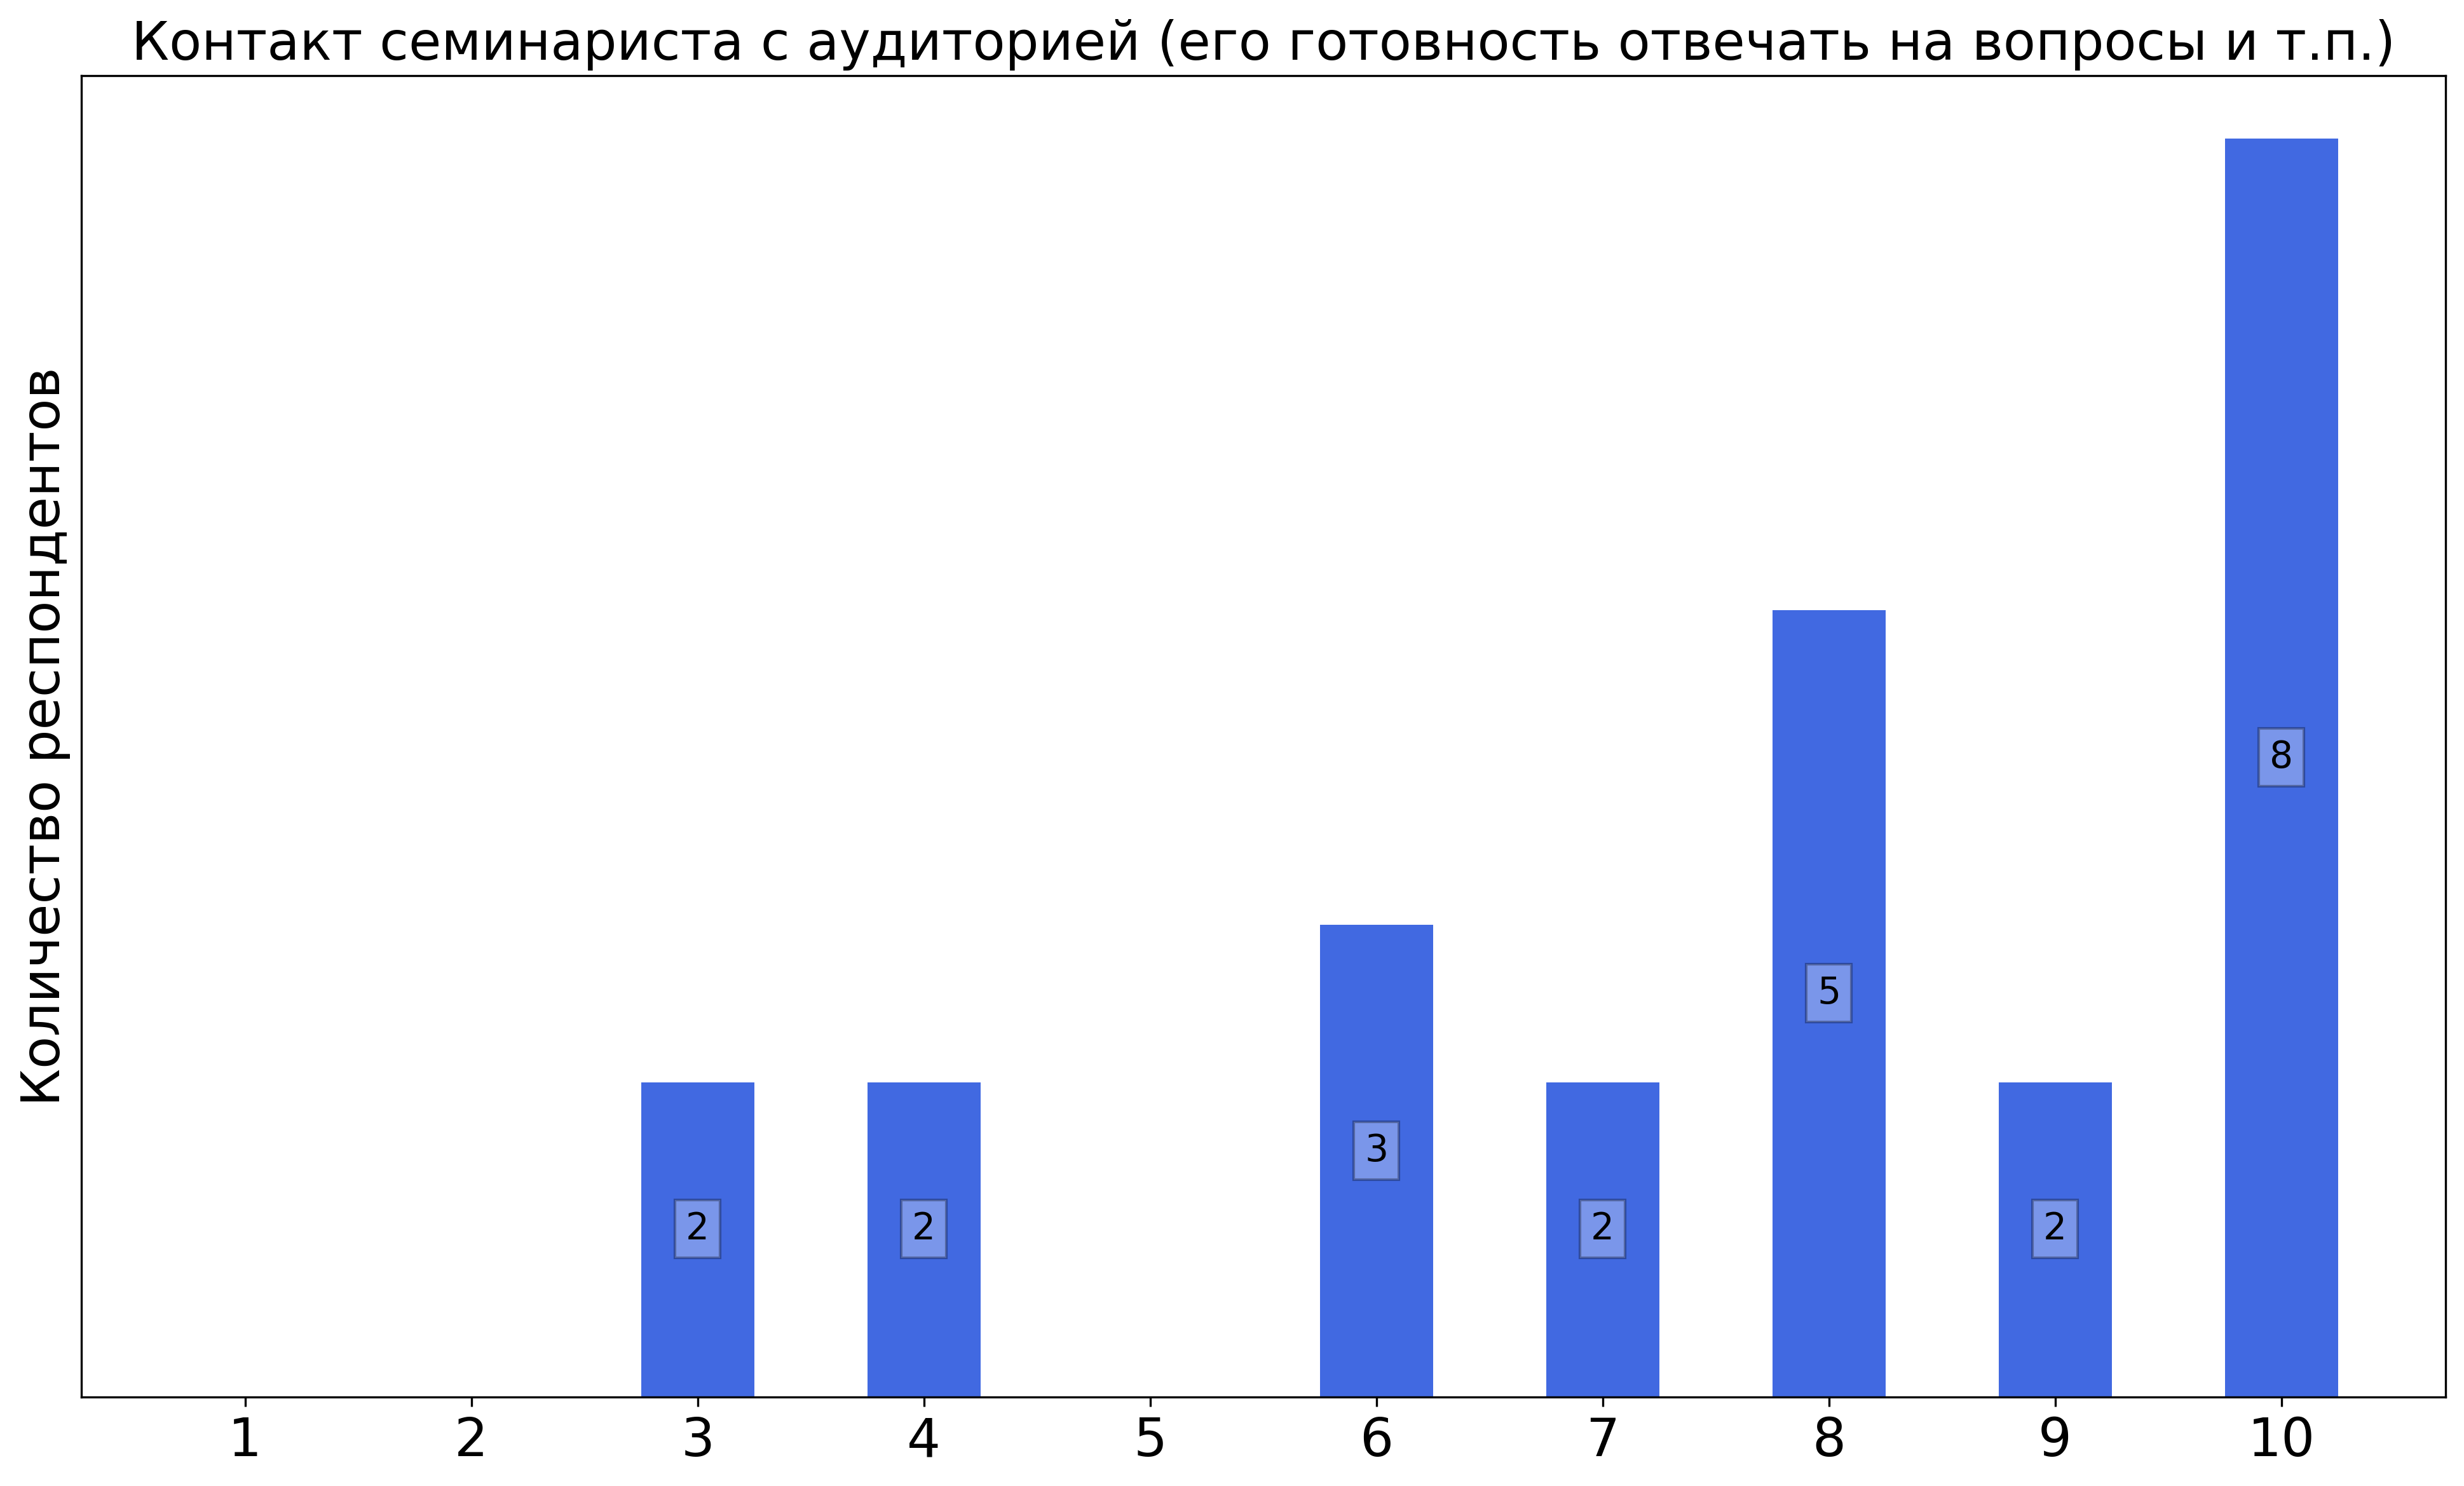
\includegraphics[width=\textwidth]{images/1 course/Дискретный анализ/seminarists-marks-Бурцев А.А.-0.png}
			\end{subfigure}
			\begin{subfigure}[b]{0.45\textwidth}
				\centering
				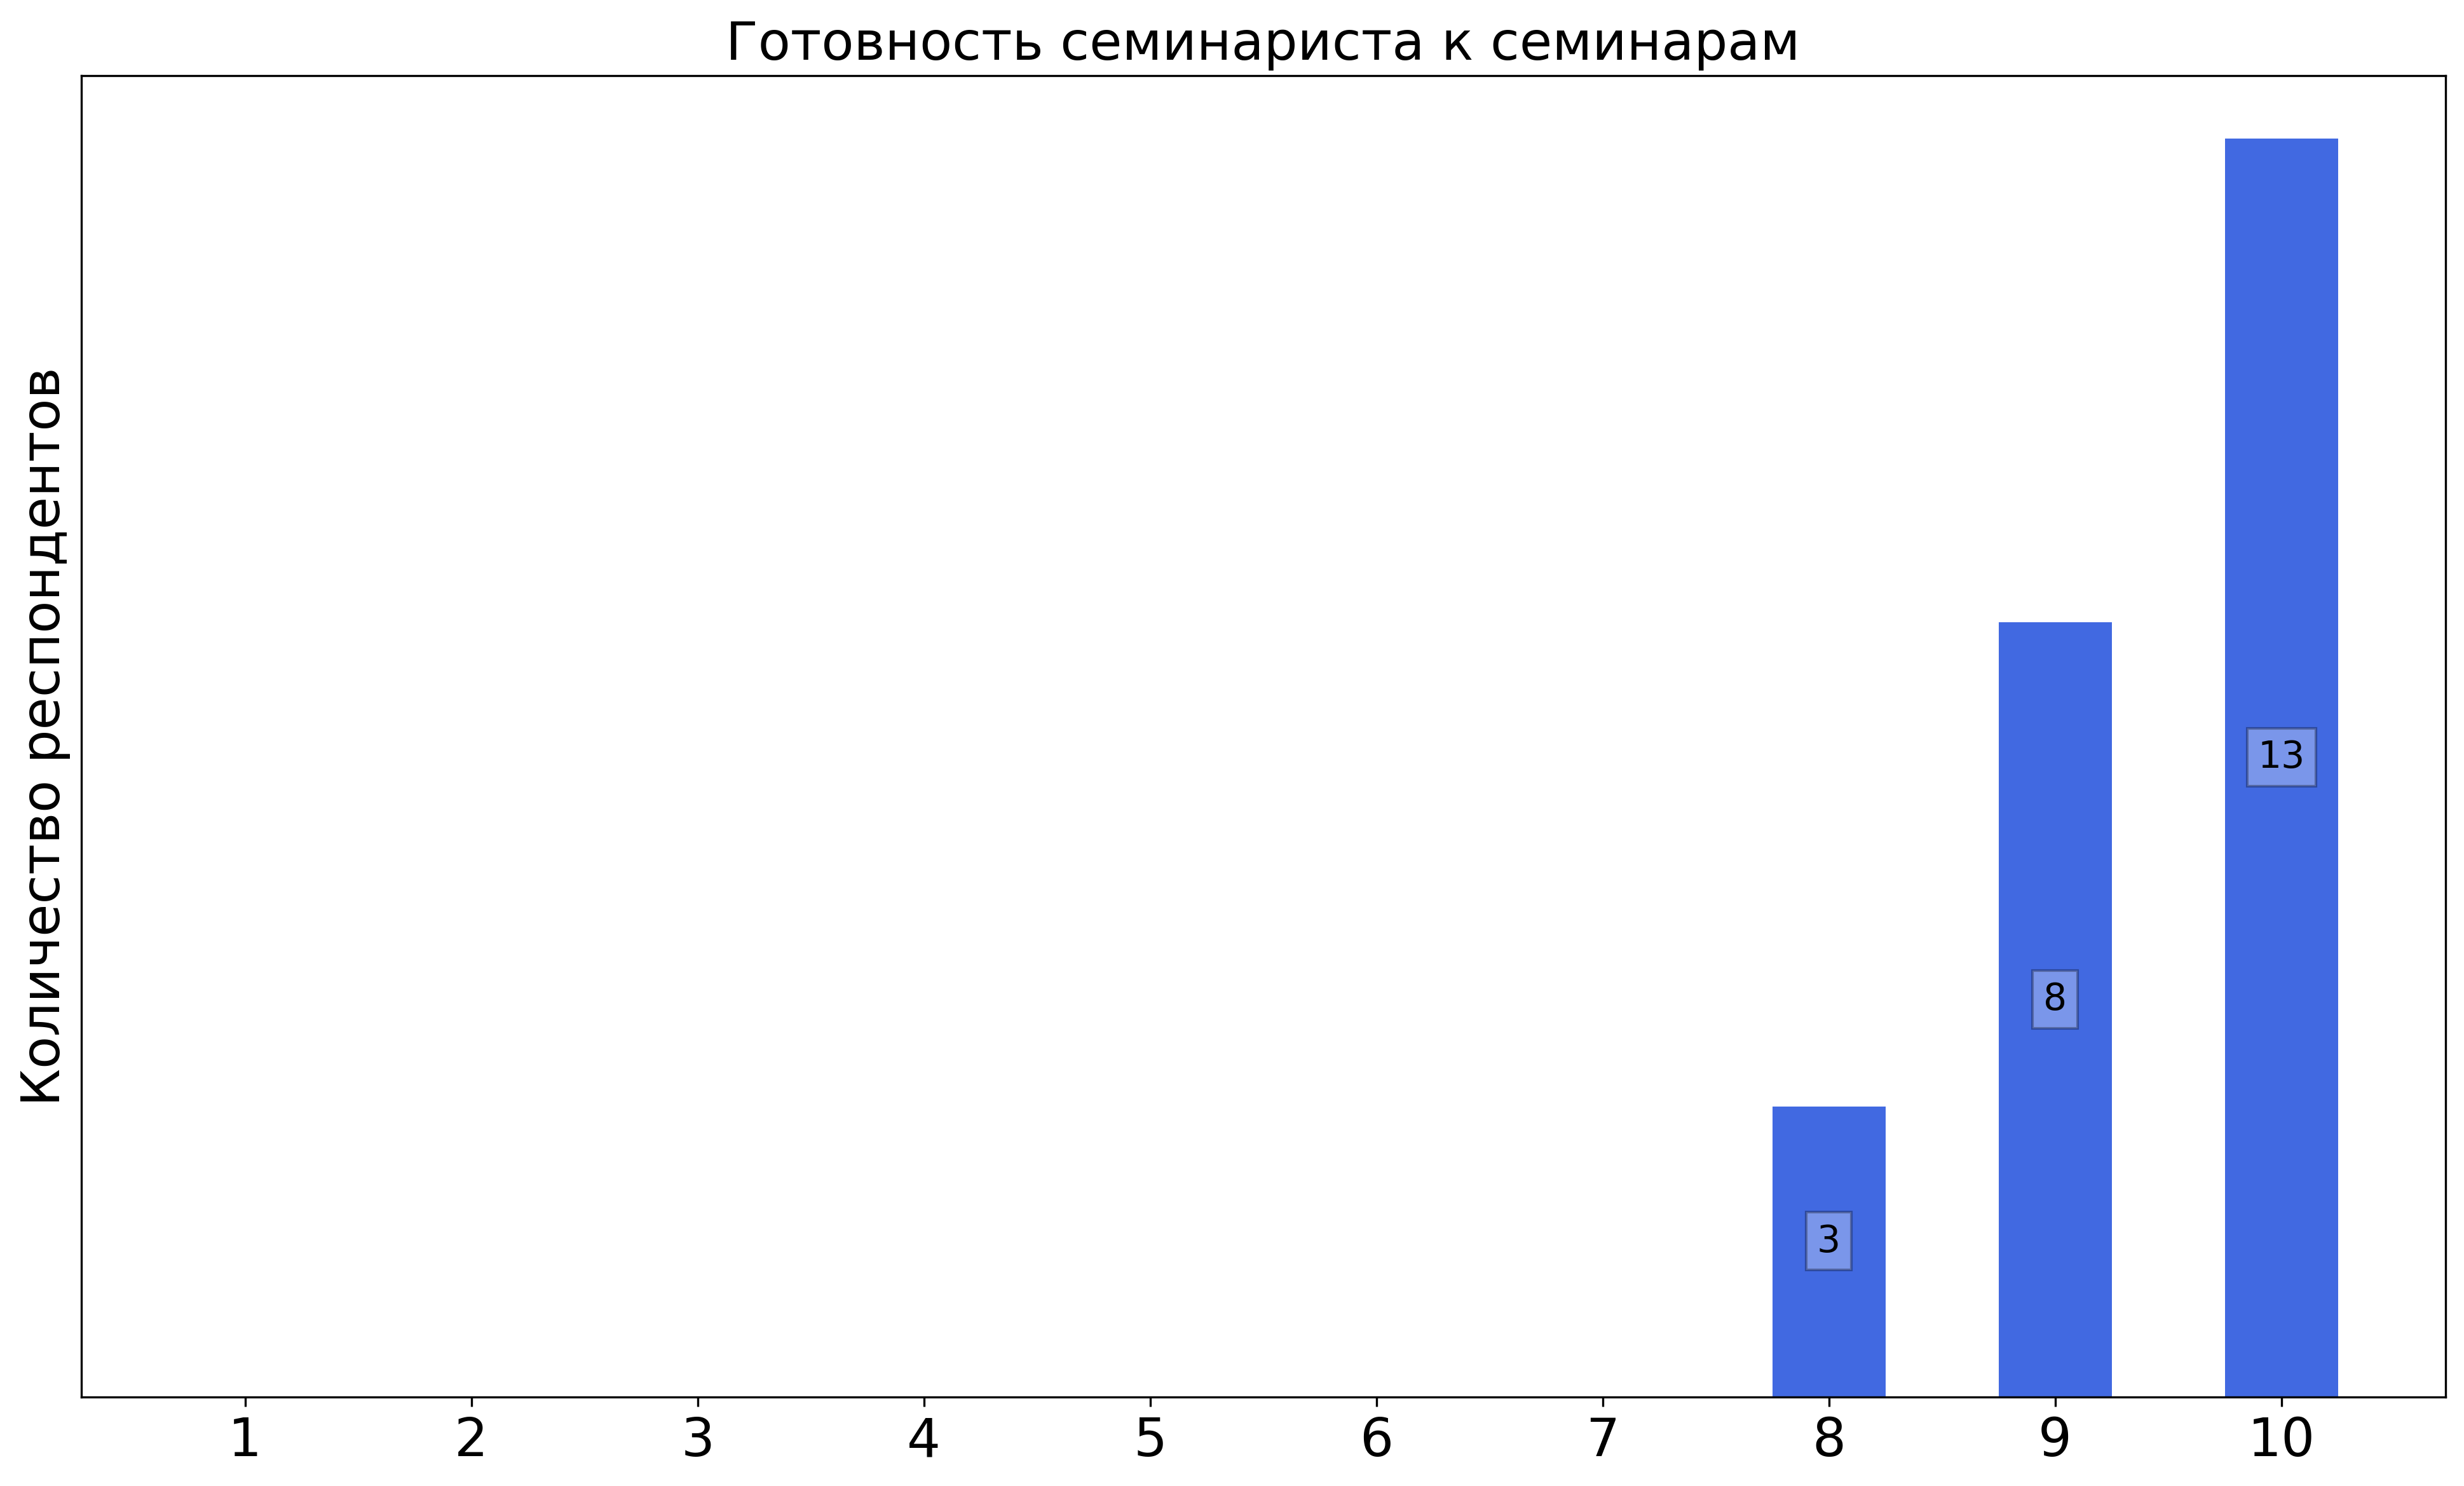
\includegraphics[width=\textwidth]{images/1 course/Дискретный анализ/seminarists-marks-Бурцев А.А.-1.png}
			\end{subfigure}
			\begin{subfigure}[b]{0.45\textwidth}
				\centering
				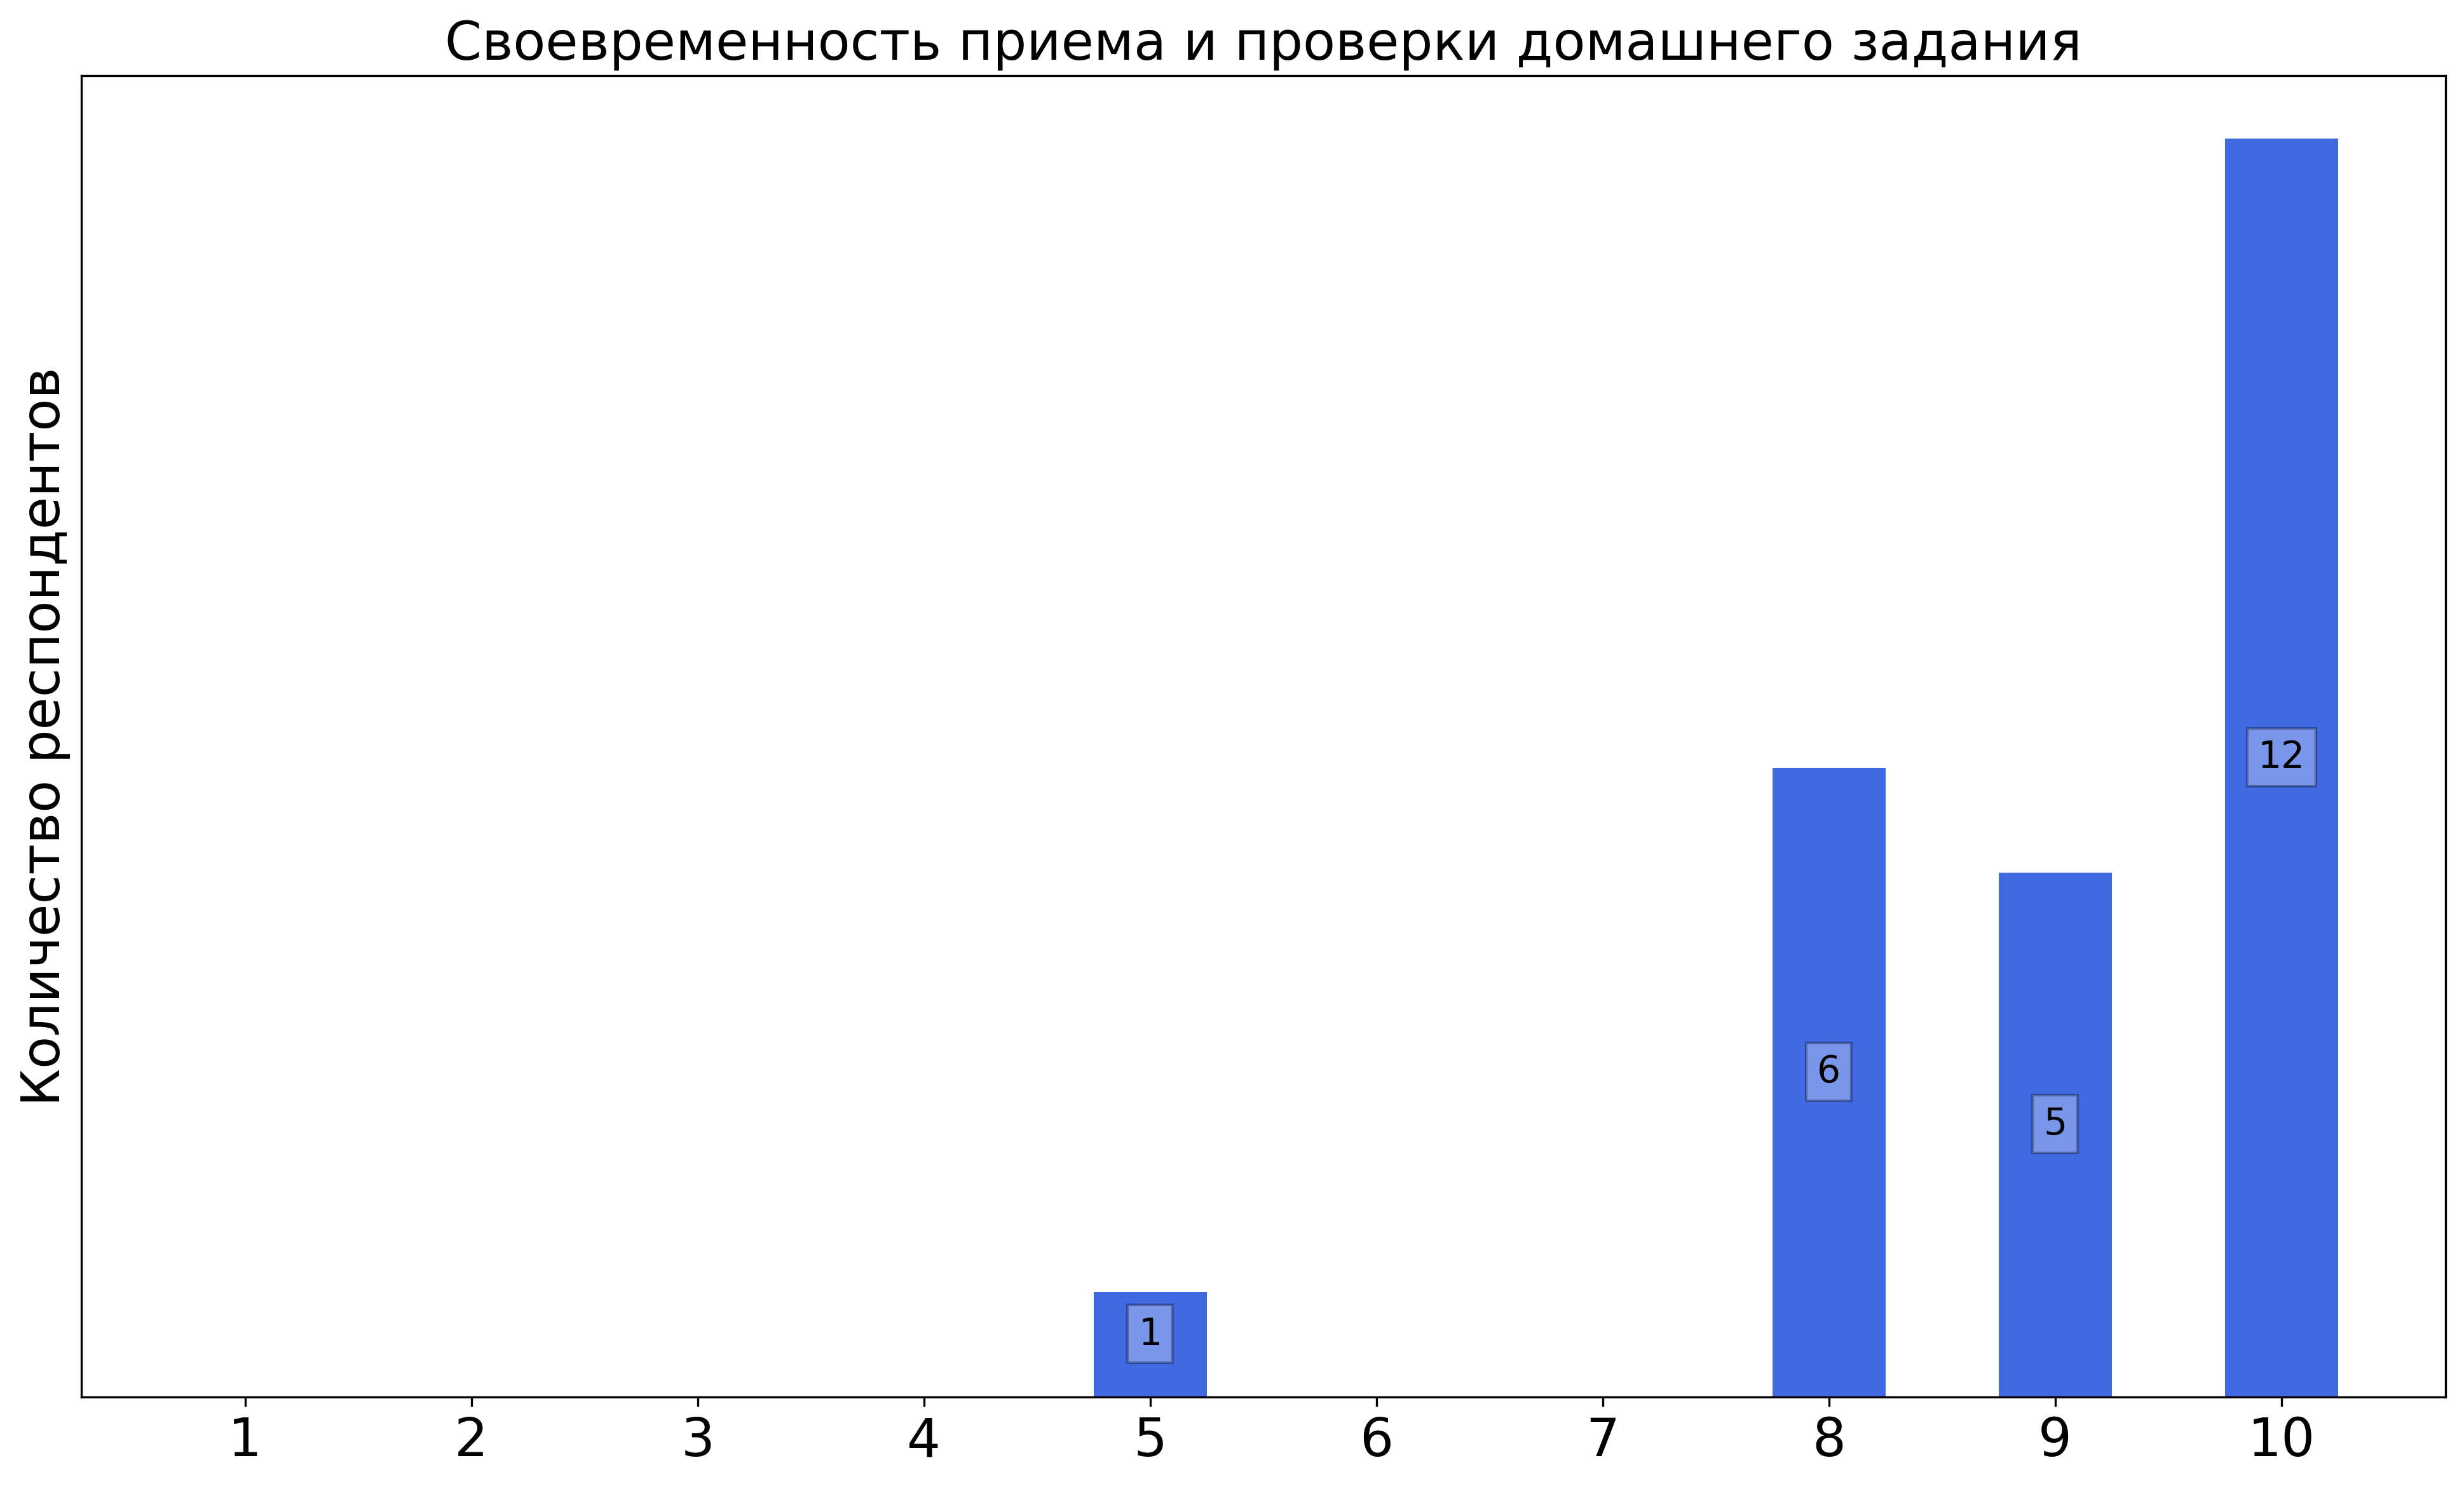
\includegraphics[width=\textwidth]{images/1 course/Дискретный анализ/seminarists-marks-Бурцев А.А.-2.png}
			\end{subfigure}
			\begin{subfigure}[b]{0.45\textwidth}
				\centering
				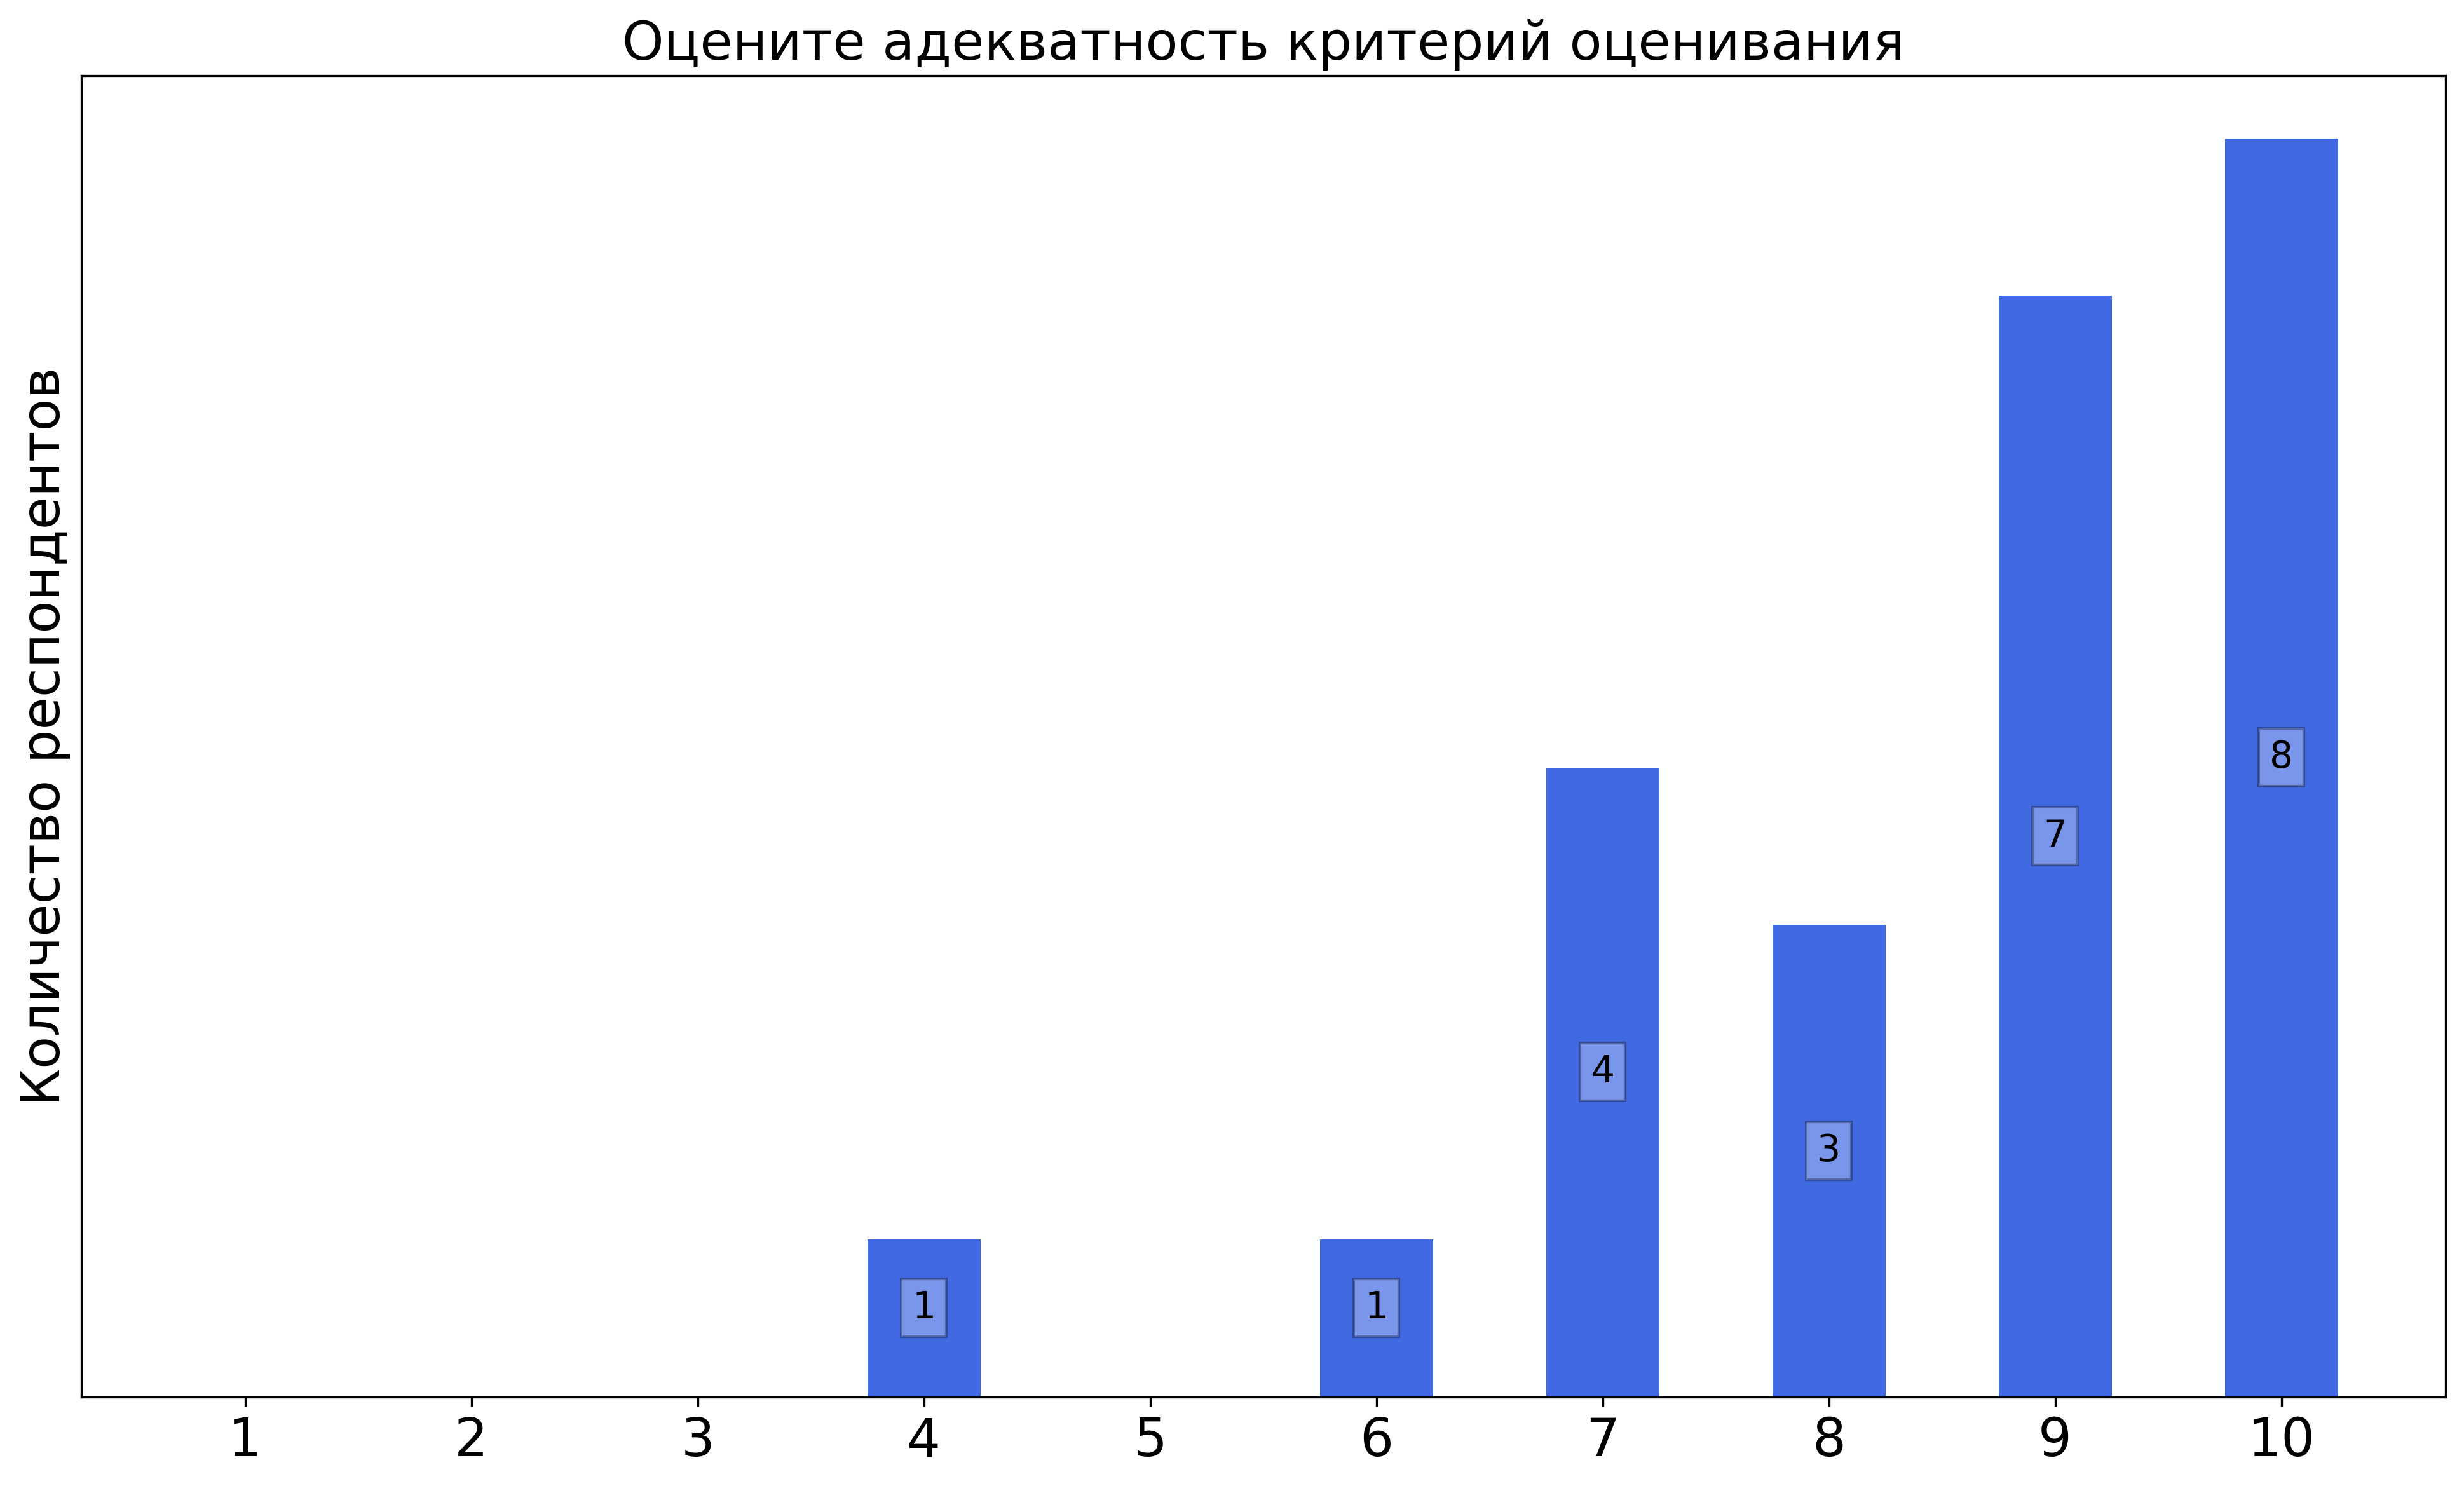
\includegraphics[width=\textwidth]{images/1 course/Дискретный анализ/seminarists-marks-Бурцев А.А.-3.png}
			\end{subfigure}	
			\caption{Оценки респондентов о качестве преподавания семинаров}
		\end{figure}

		\textbf{Комментарии студентов о семинаристе\protect\footnote{сохранены оригинальные орфография и пунктуация}}
            \begin{commentbox} 
                Семинары превращались в лекции, на которых семинарист рассказывал что-то своё, отличное от общей программы. В начале рассказал булеву алгебру, затем свой собственный курс "математическая кибернетика". Провел одну контрольную, оценки всем поставил хорошие. 
            \end{commentbox} 
            
            \begin{commentbox} 
                Поначалу лекции с семами совпадали, потом он начал читать что-то другое и непонятное, потом вообще начал читать свой курс, но за него он дополнительно всем 10 вроде поставил, так что халявный. Но по итогу базы, по типу теории графов, комбинаторики, мы не узнали, поэтому не кайф. 
            \end{commentbox} 
            
            \begin{commentbox} 
                Очень умный и приятный человек. Было большим наслаждением слушать семинариста. 
            \end{commentbox} 
            
            \begin{commentbox} 
                Графы и комбинаторику не трогали совсем, что несколько огорчает, вторая половина семестра - его доп по математическим основам кибернетики, из которого понятно было в среднем 60\% сказанного. Семинары больше в формате лекций. Однако закрываться на отл было более чем просто (кр по кибернетике не было), грех жаловаться. 
            \end{commentbox} 
            
            \begin{commentbox} 
                Не очень понятно ведёт семинары из-за скорости и почерка, но в целом можно задавать вопросы и становится яснее 
            \end{commentbox} 
            
            \begin{commentbox} 
                Большая часть времени уделялась изложению собственного курса семинариста: "Математическая кибернетика". Материал довольно сложный, но интересный 
            \end{commentbox} 
            
            \begin{commentbox} 
                Рассказывает свою программу, которая почти не связана с лекционным курсом. Понять многие моменты можно с трудом, но отл поставит за то, что ты умеешь дышать.  
            \end{commentbox} 
            
            \begin{commentbox} 
                Вёл совсем другой предмет, на семинарах в основном "читал лекции", задач решали очень мало... Хоть было и интересно, его подача была не очень сбалансированна... Хотелось бы согласования с лекциями и больше практики 
            \end{commentbox} 


    \subsubsection{Отзыв студентов о семинарах. Семинарист: Савельев А.В.}
        \begin{figure}[H]
            \centering
            \begin{subfigure}[b]{0.45\textwidth}
                \centering
                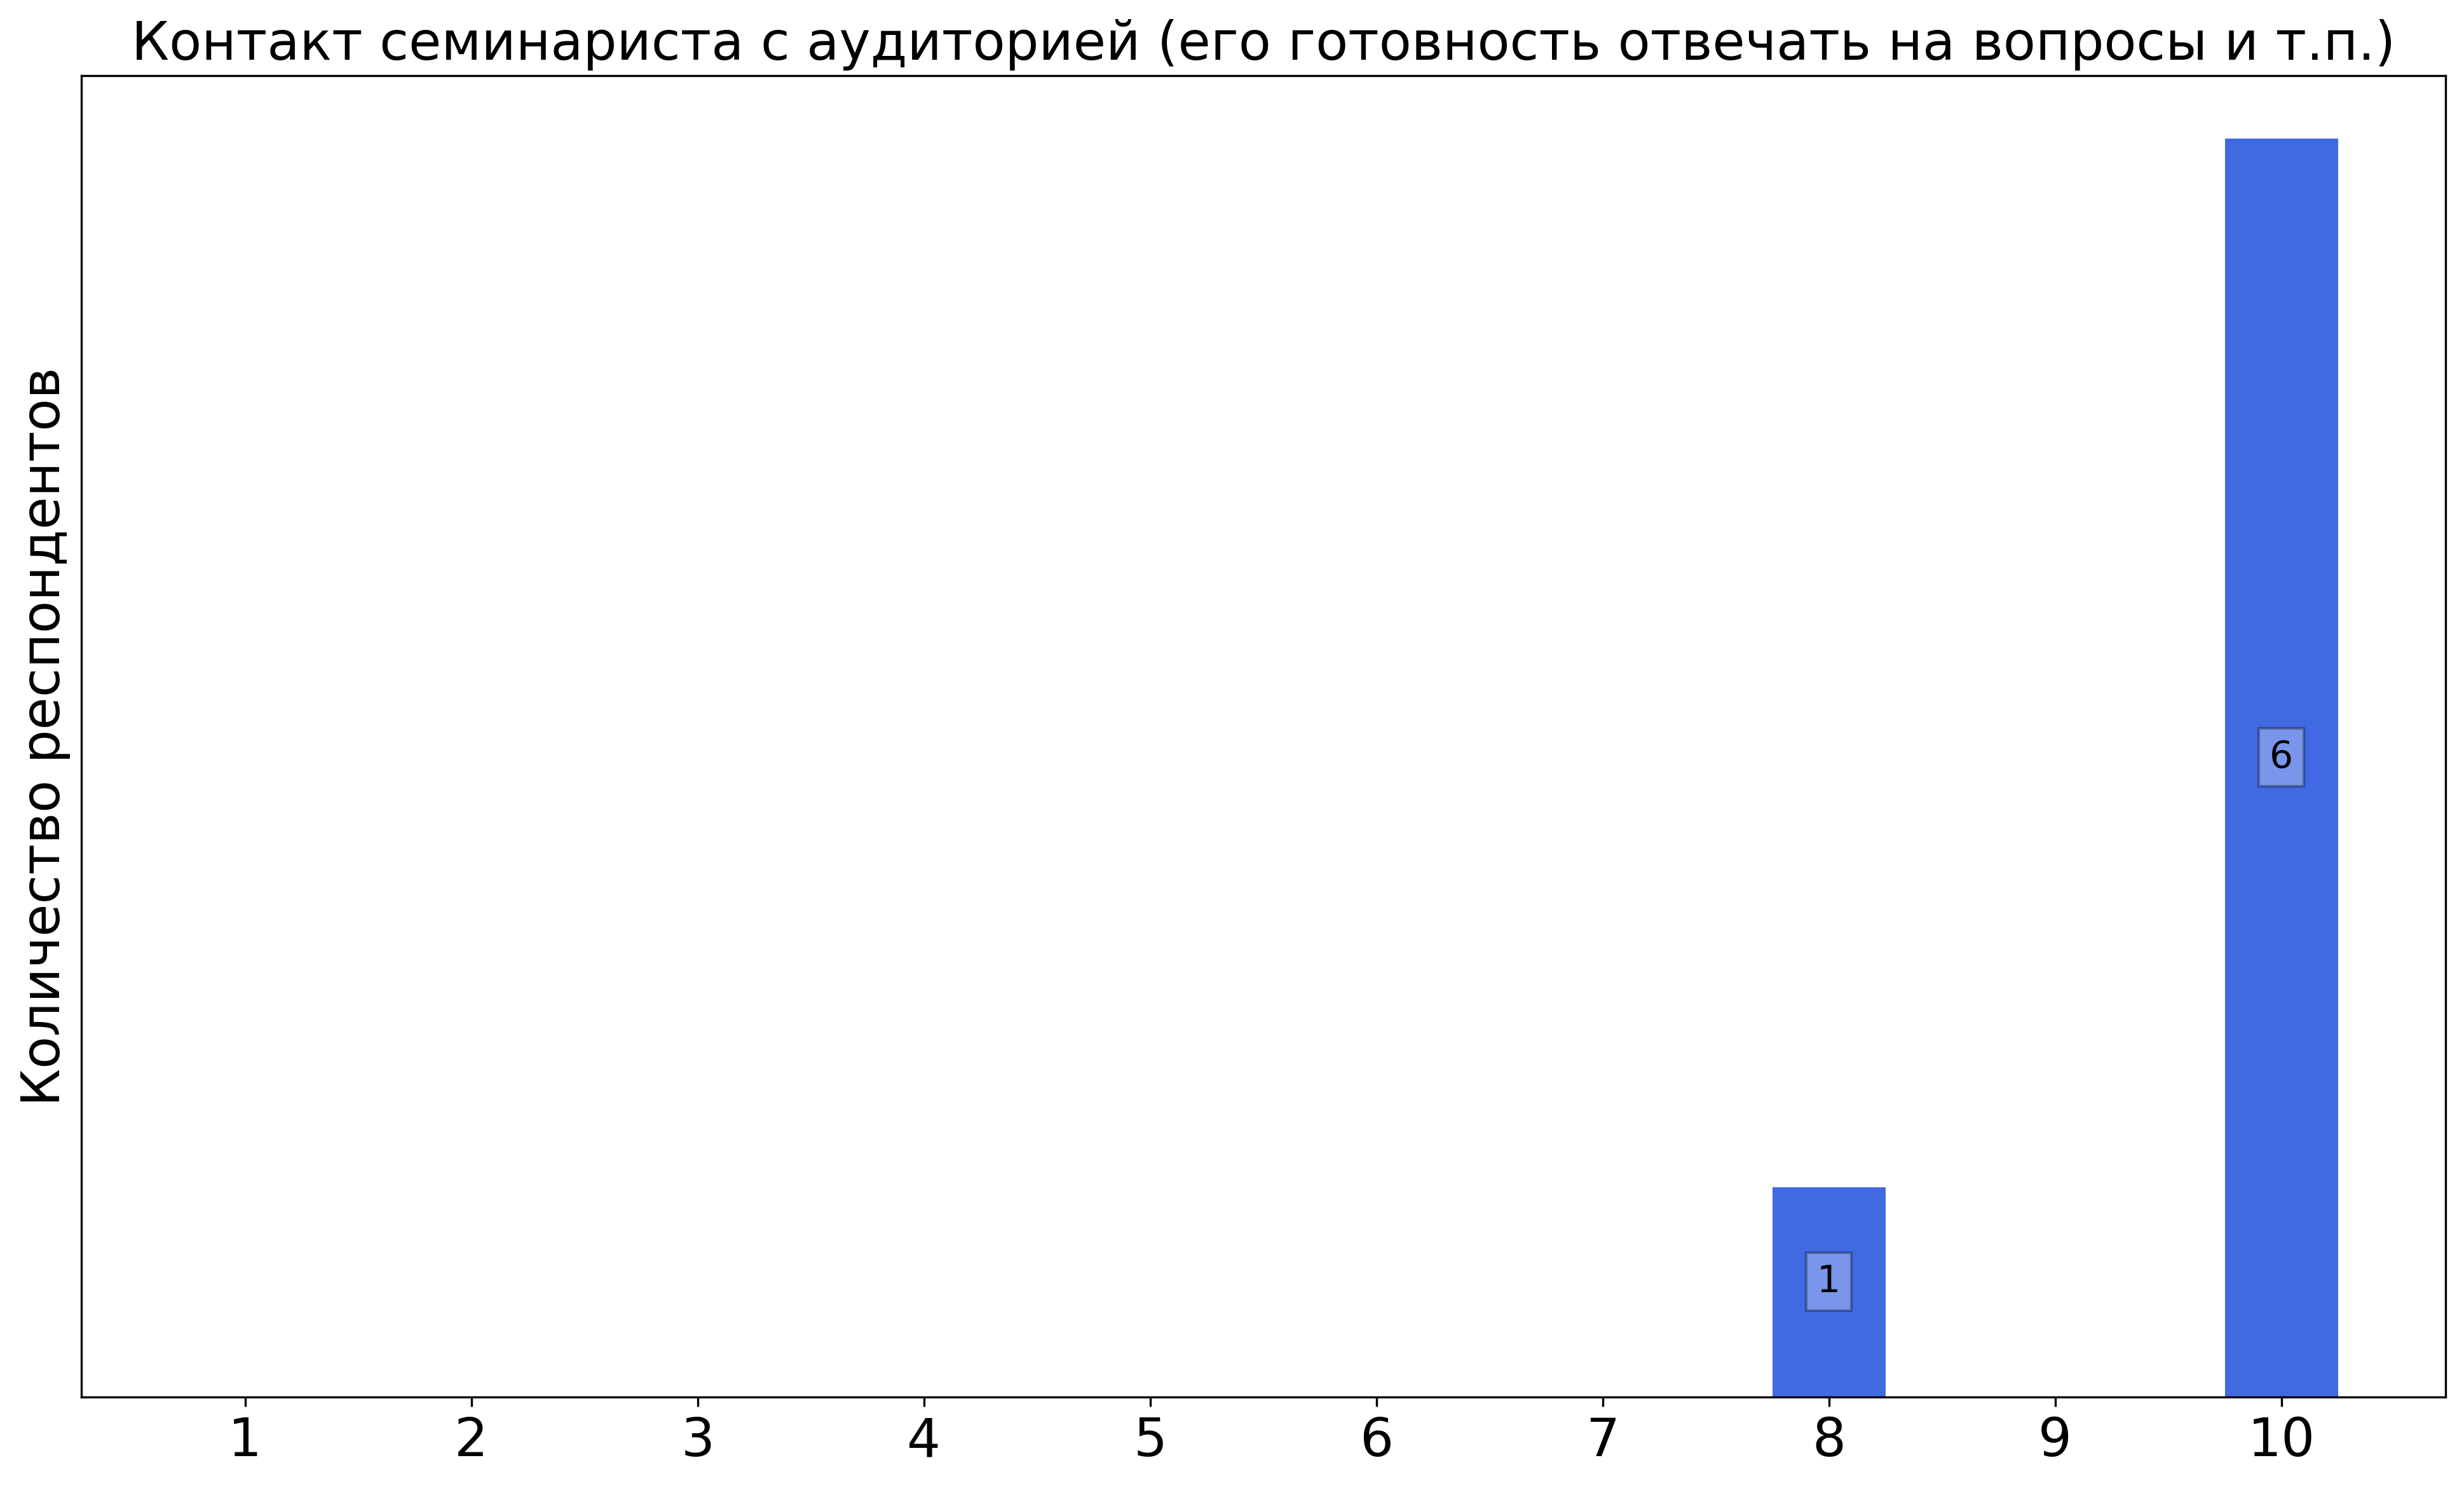
\includegraphics[width=\textwidth]{images/1 course/Дискретный анализ/seminarists-marks-Савельев А.В.-0.png}
            \end{subfigure}
            \begin{subfigure}[b]{0.45\textwidth}
                \centering
                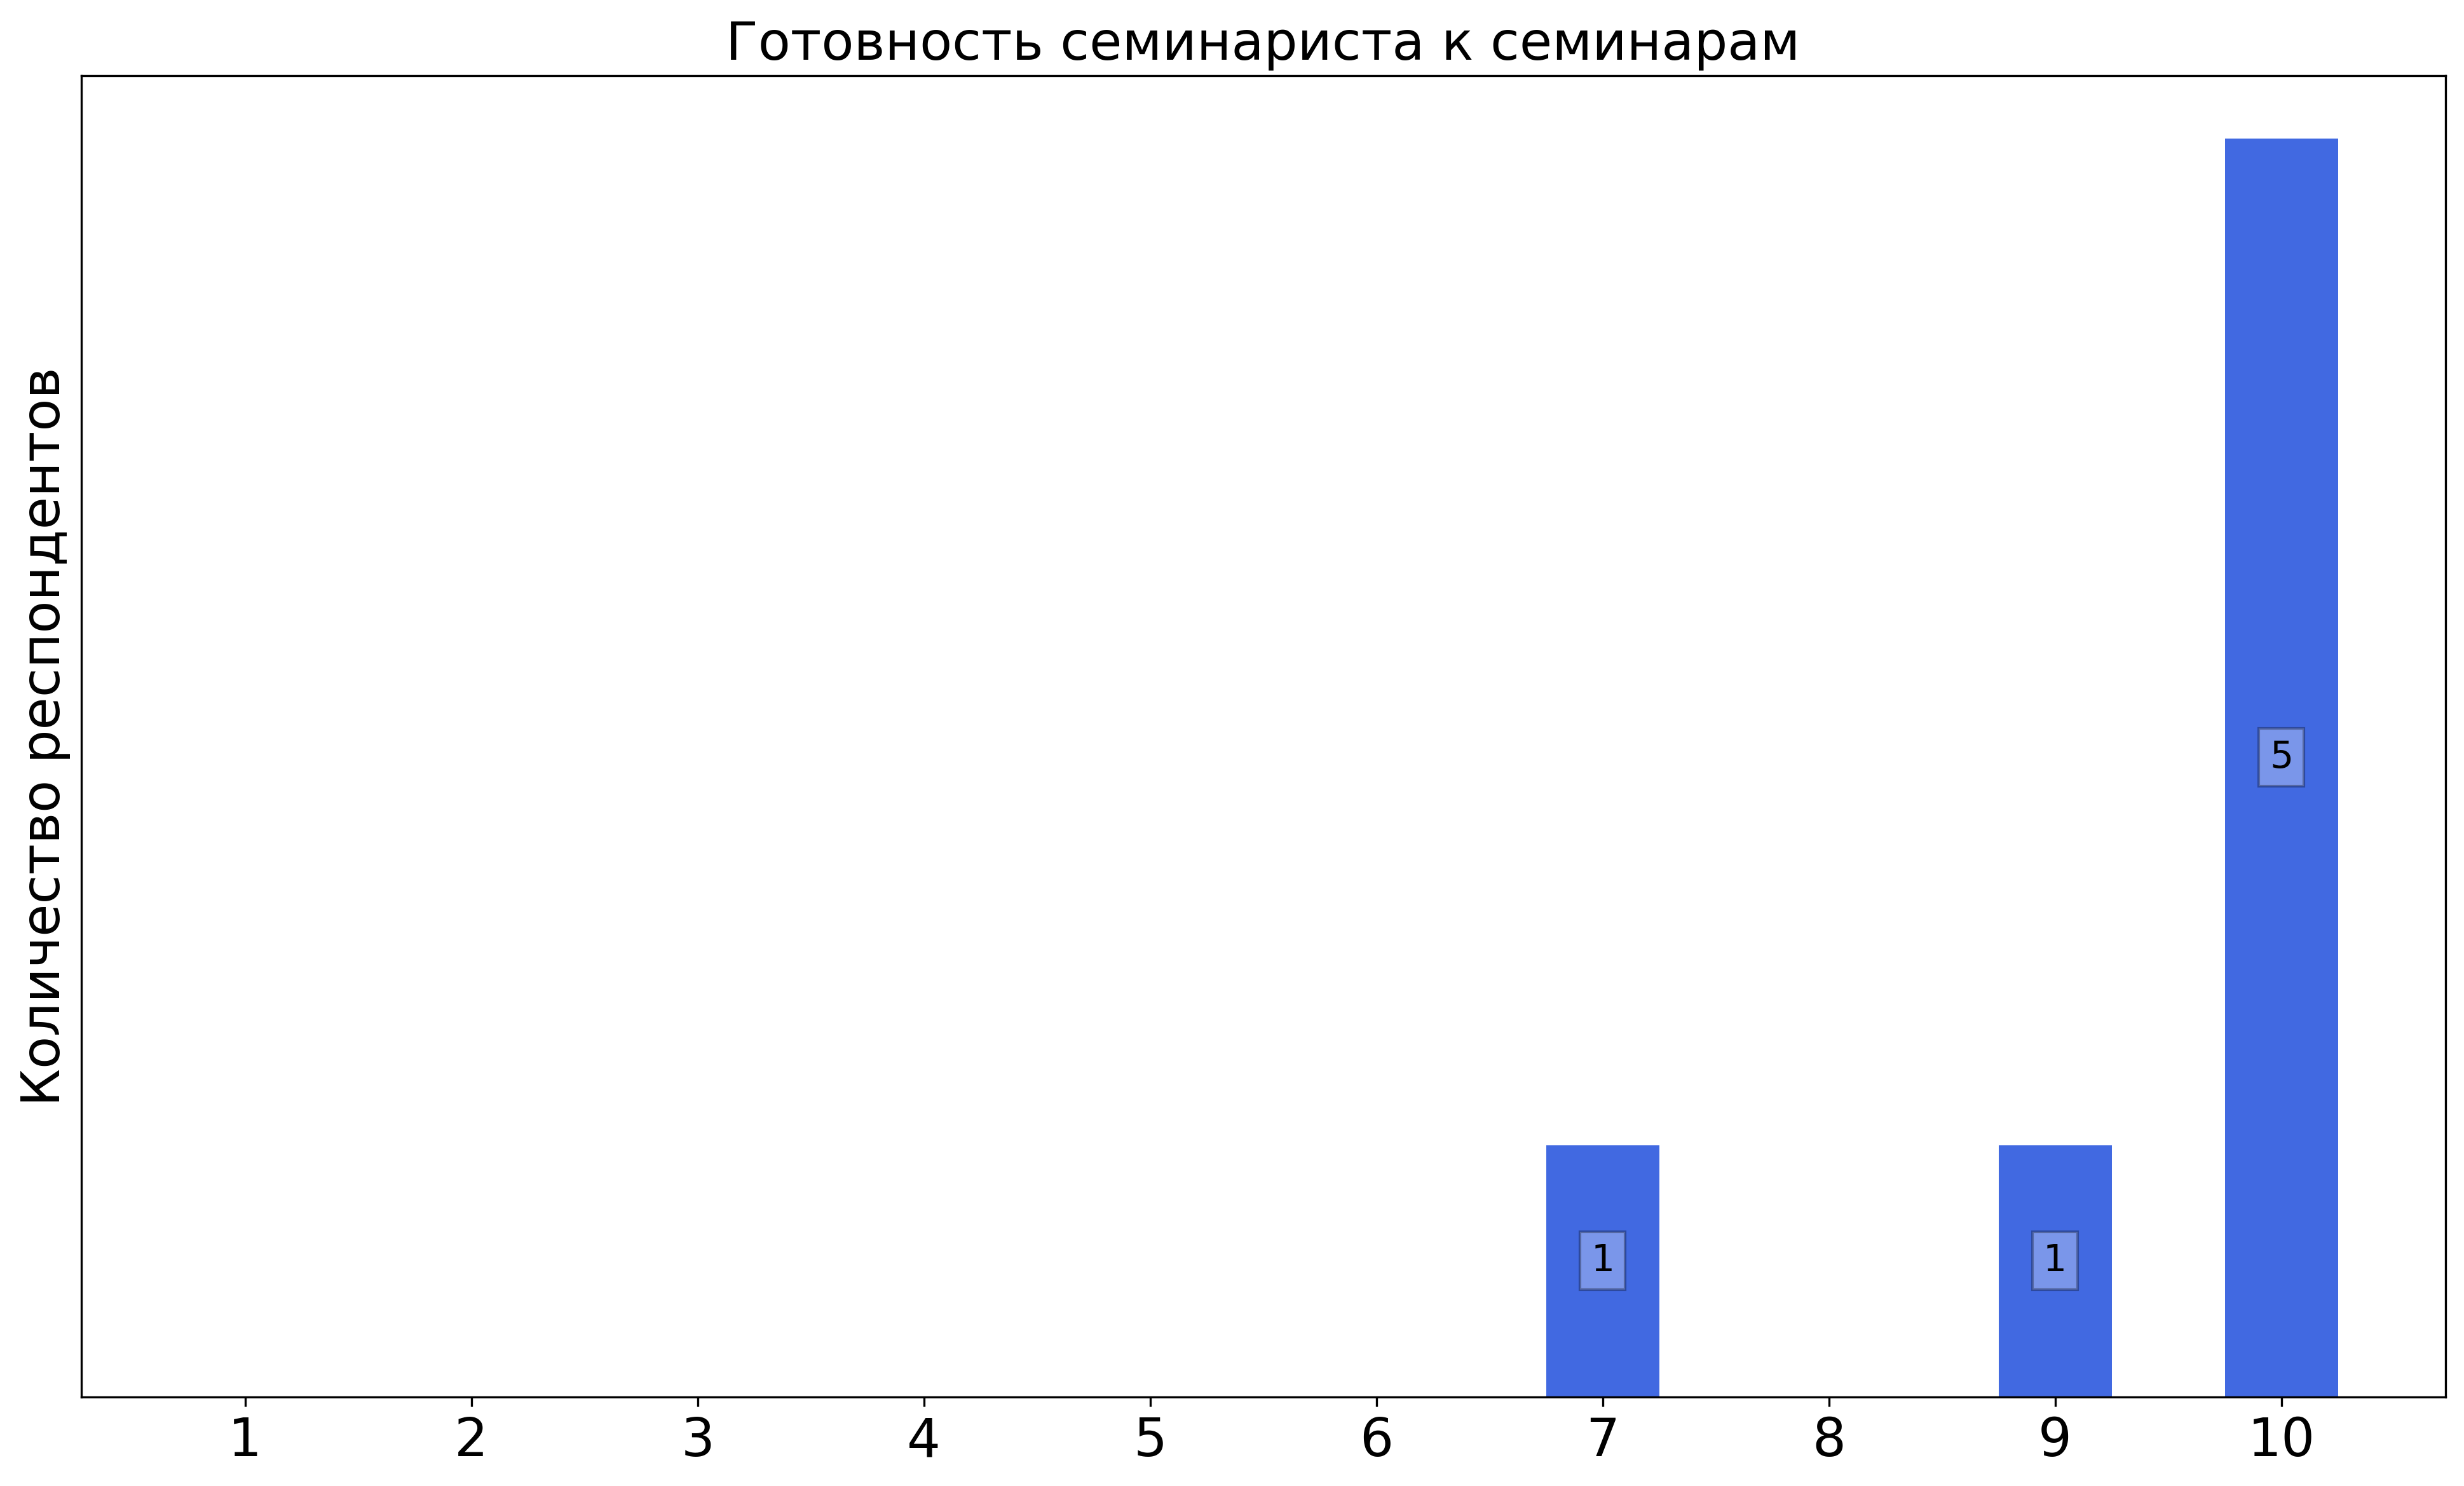
\includegraphics[width=\textwidth]{images/1 course/Дискретный анализ/seminarists-marks-Савельев А.В.-1.png}
            \end{subfigure}
            \begin{subfigure}[b]{0.45\textwidth}
                \centering
                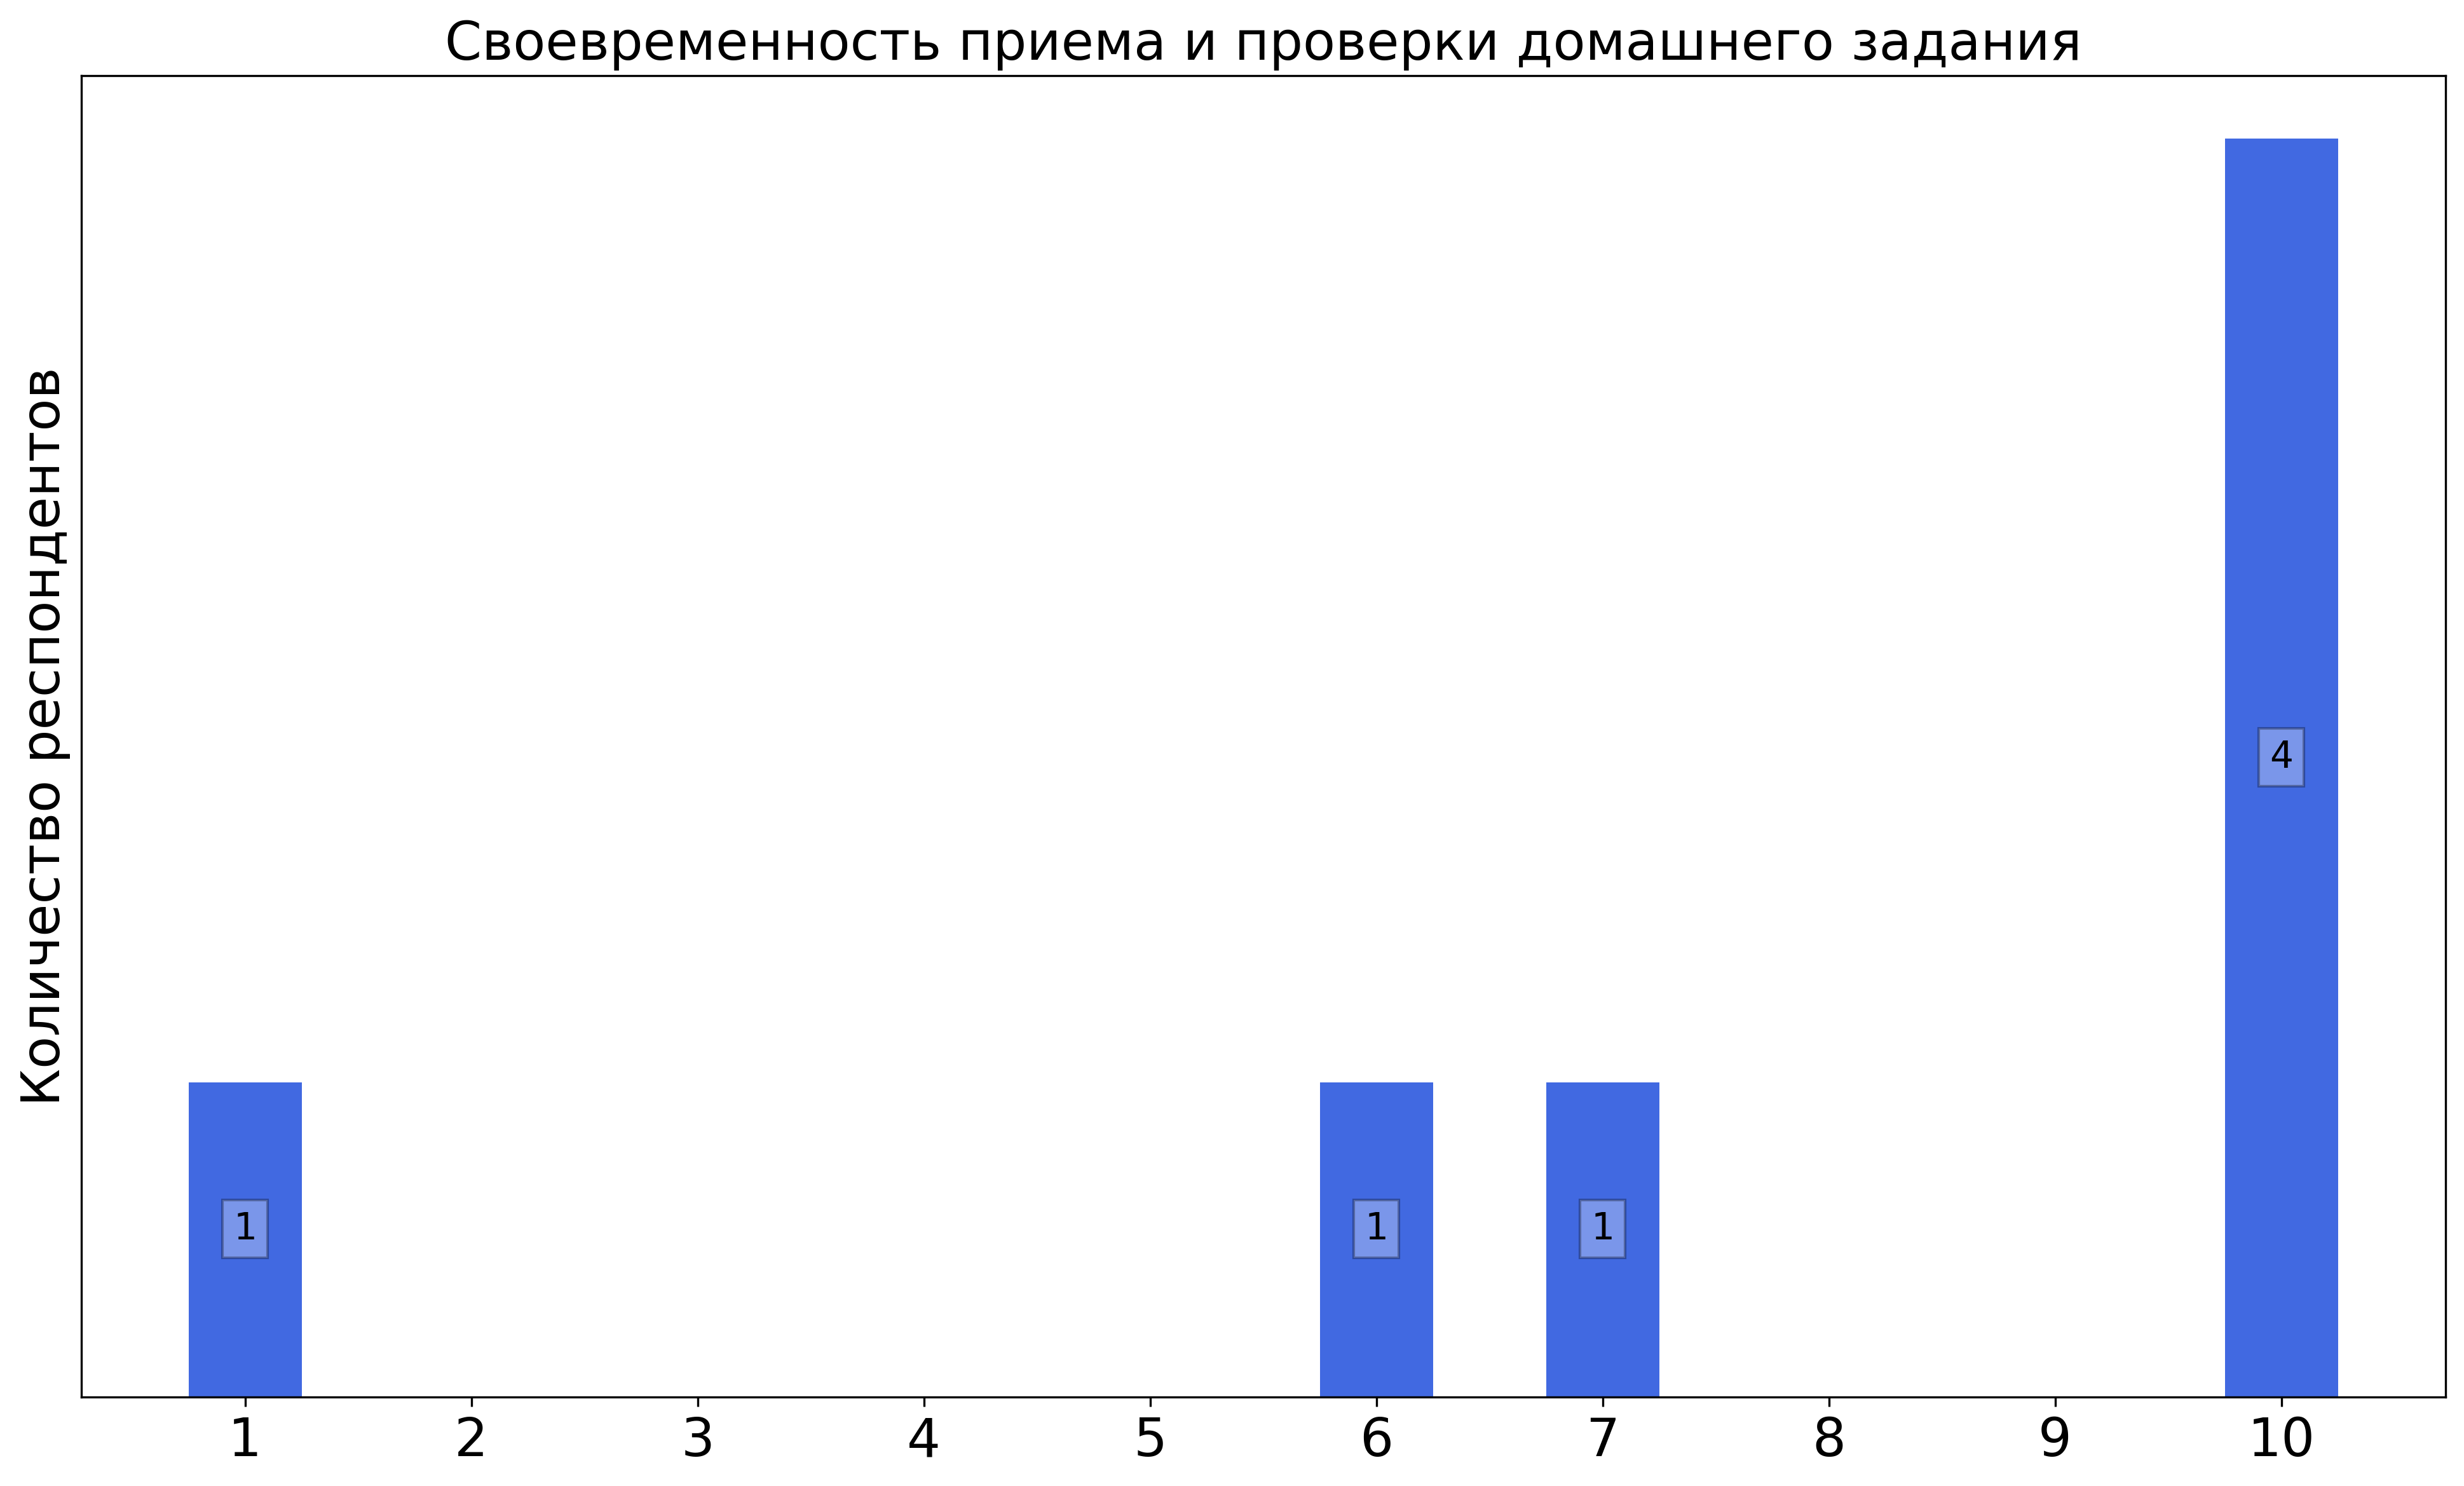
\includegraphics[width=\textwidth]{images/1 course/Дискретный анализ/seminarists-marks-Савельев А.В.-2.png}
            \end{subfigure}
            \begin{subfigure}[b]{0.45\textwidth}
                \centering
                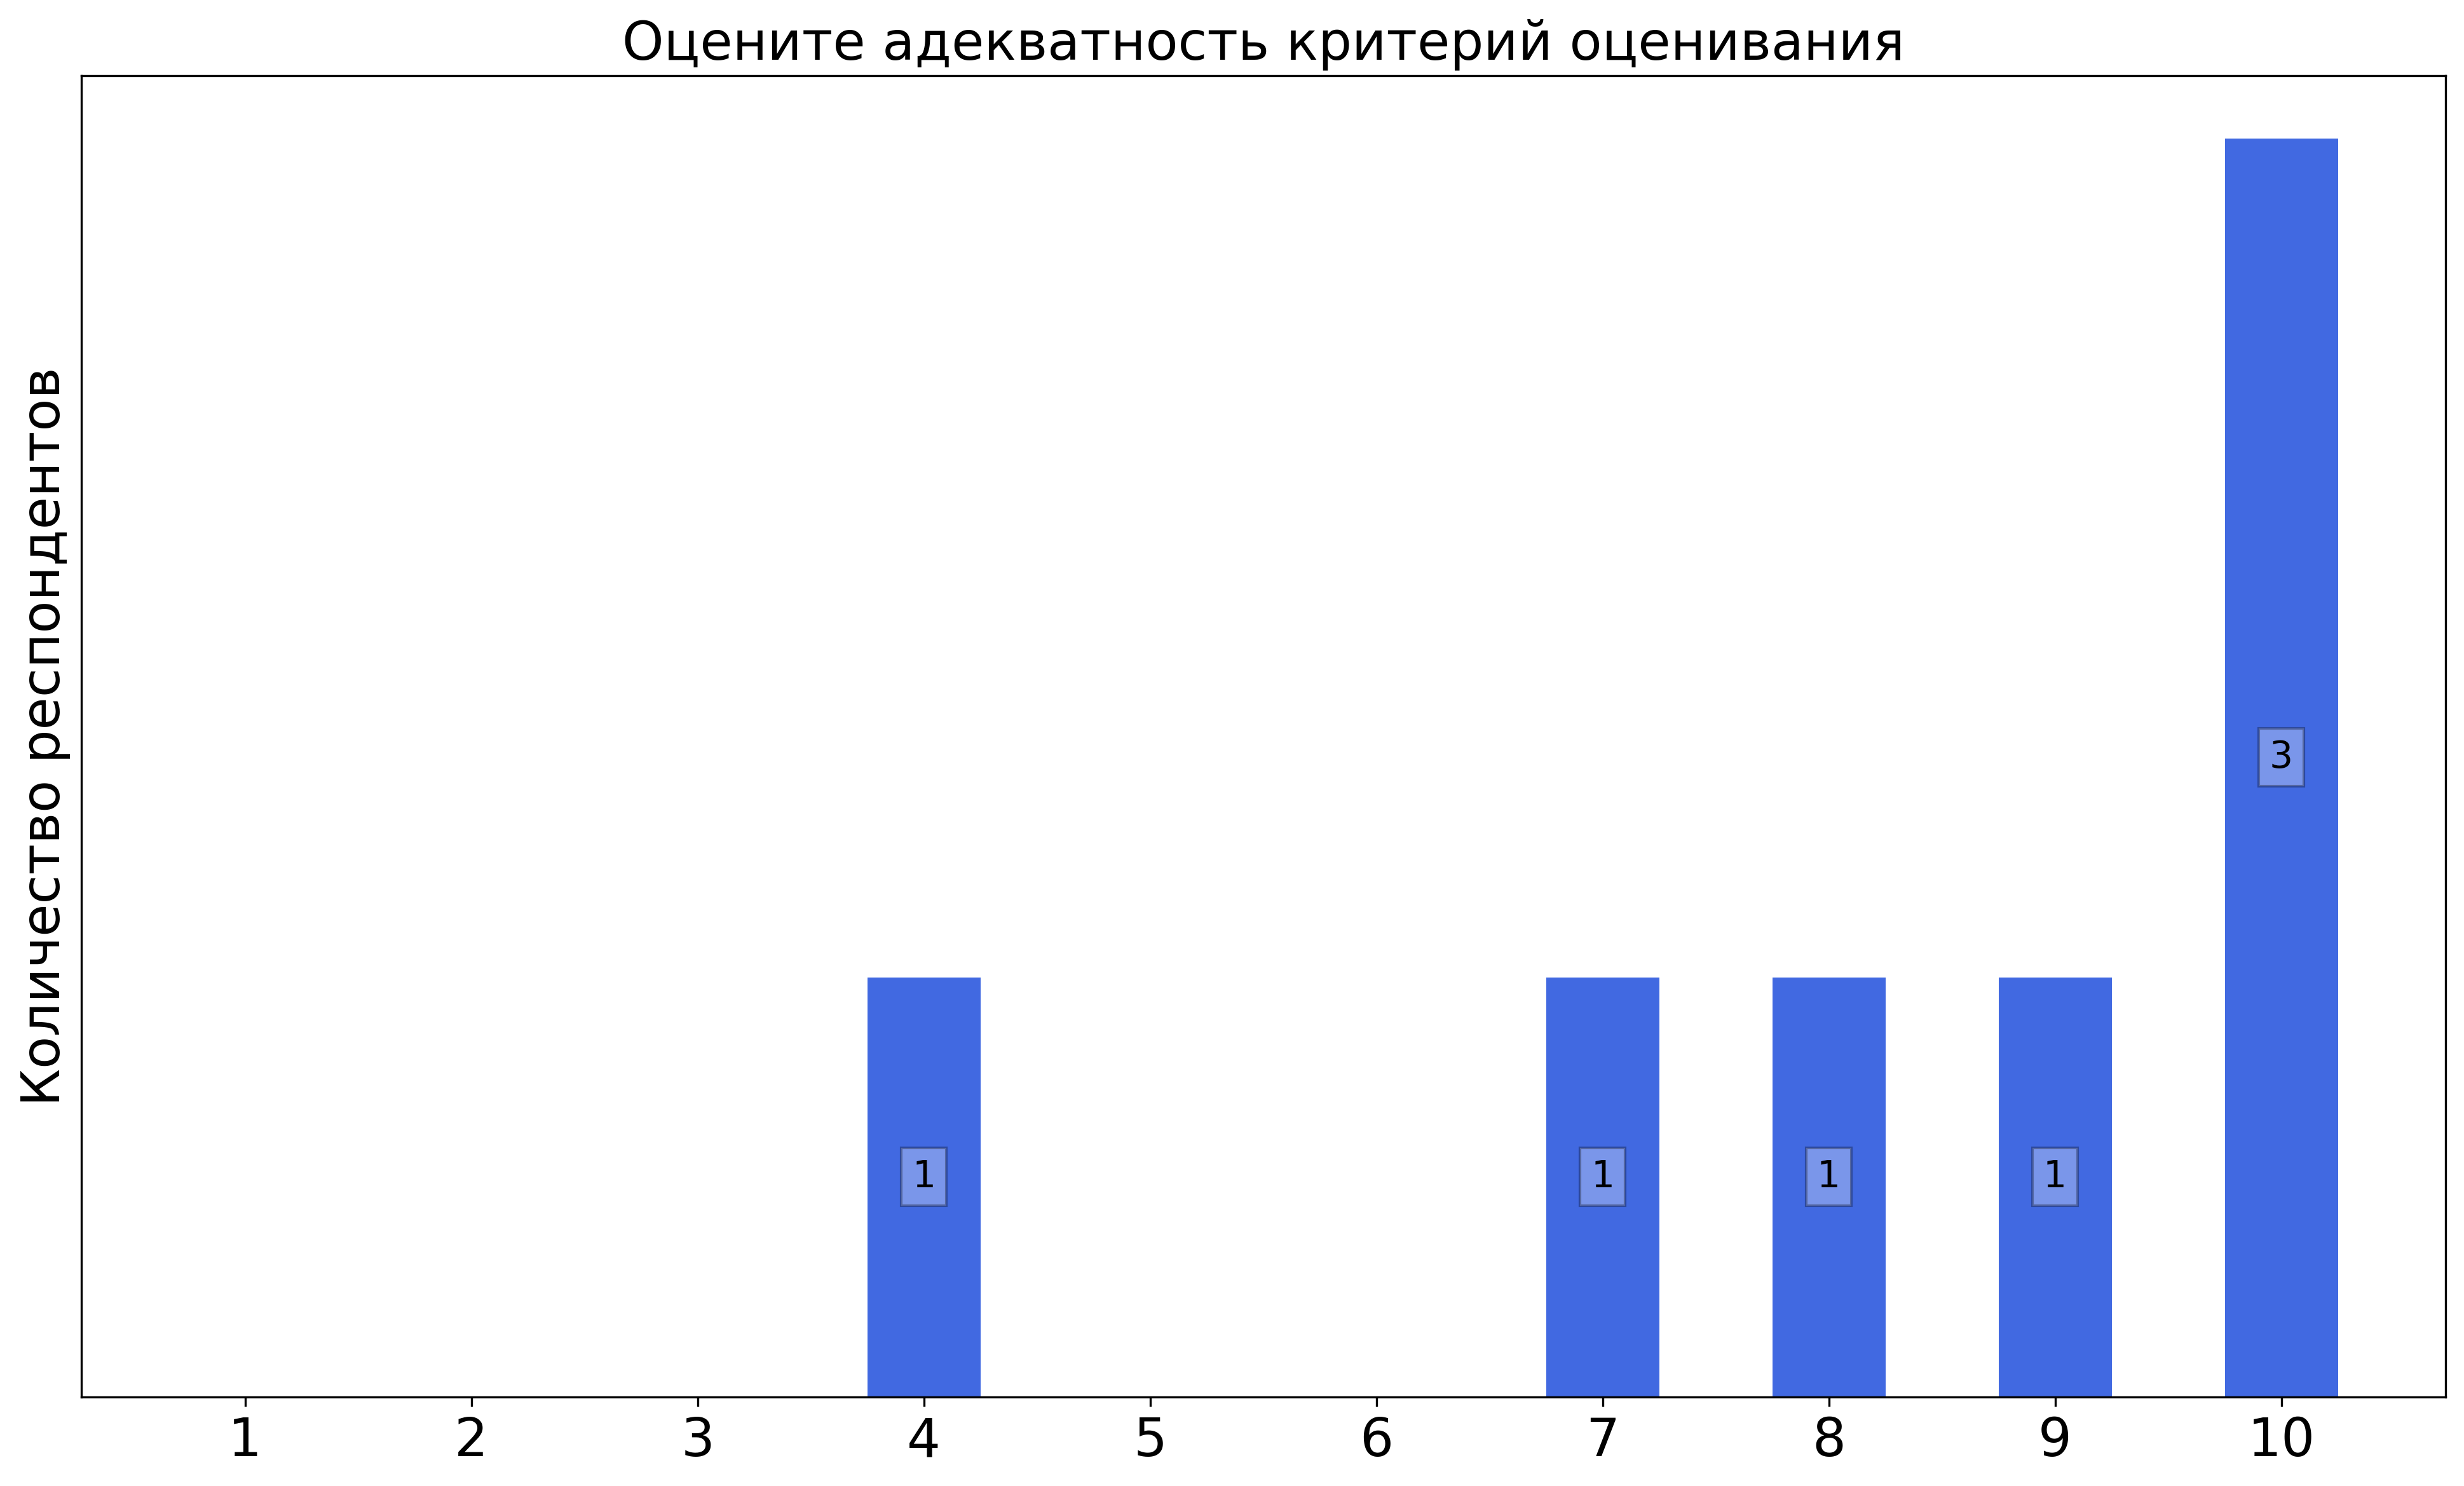
\includegraphics[width=\textwidth]{images/1 course/Дискретный анализ/seminarists-marks-Савельев А.В.-3.png}
            \end{subfigure}	
            \caption{Оценки респондентов о качестве преподавания семинаров}
        \end{figure}

        \textbf{Комментарии студентов о семинаристе\protect\footnote{сохранены оригинальные орфография и пунктуация}}
            \begin{commentbox} 
                Всё здорово. Программу освоил по одним только по семинарам. Спасибо Александру Викторовичу! 
            \end{commentbox} 
        
            \begin{commentbox} 
                Практически всегда пара по дискретке у нас длилась не до 20.00, а до 21 и позже. И то мы под конец уже начинали ныть, что ничего не соображаем, а так семинарист был готов продолжить решать задачи до закрытия Физтеха. Критерии оценивания на зачёте у него очень странные, ставил оценки на обум. Сдача зачёта у него очень долгая. Причём он вначале сказал что для хор 6 нужно немного теории рассказать, в итоге в часов 21 все уже минимум теории рассказали, а он не хотел ставить хор 6, максимум уд 4.  Есть и плюсы, по нему видно как он горит этим делом, как он хочет нас чему-нибудь научить, он отвечает буквально на все вопросы, если не понял как решать задачу, он раз 100 готов ещё раз объяснить. Готов прийти в 7 часов утра и проводить сдачу домашки. Неходя на лекции, ты мог узнать всю информацию с семинара, настолько он хорошо рассказывал 
            \end{commentbox}


    \subsubsection{Отзыв студентов о семинарах. Семинарист: Кириков Е.}
        \begin{figure}[H]
            \centering
            \begin{subfigure}[b]{0.45\textwidth}
                \centering
                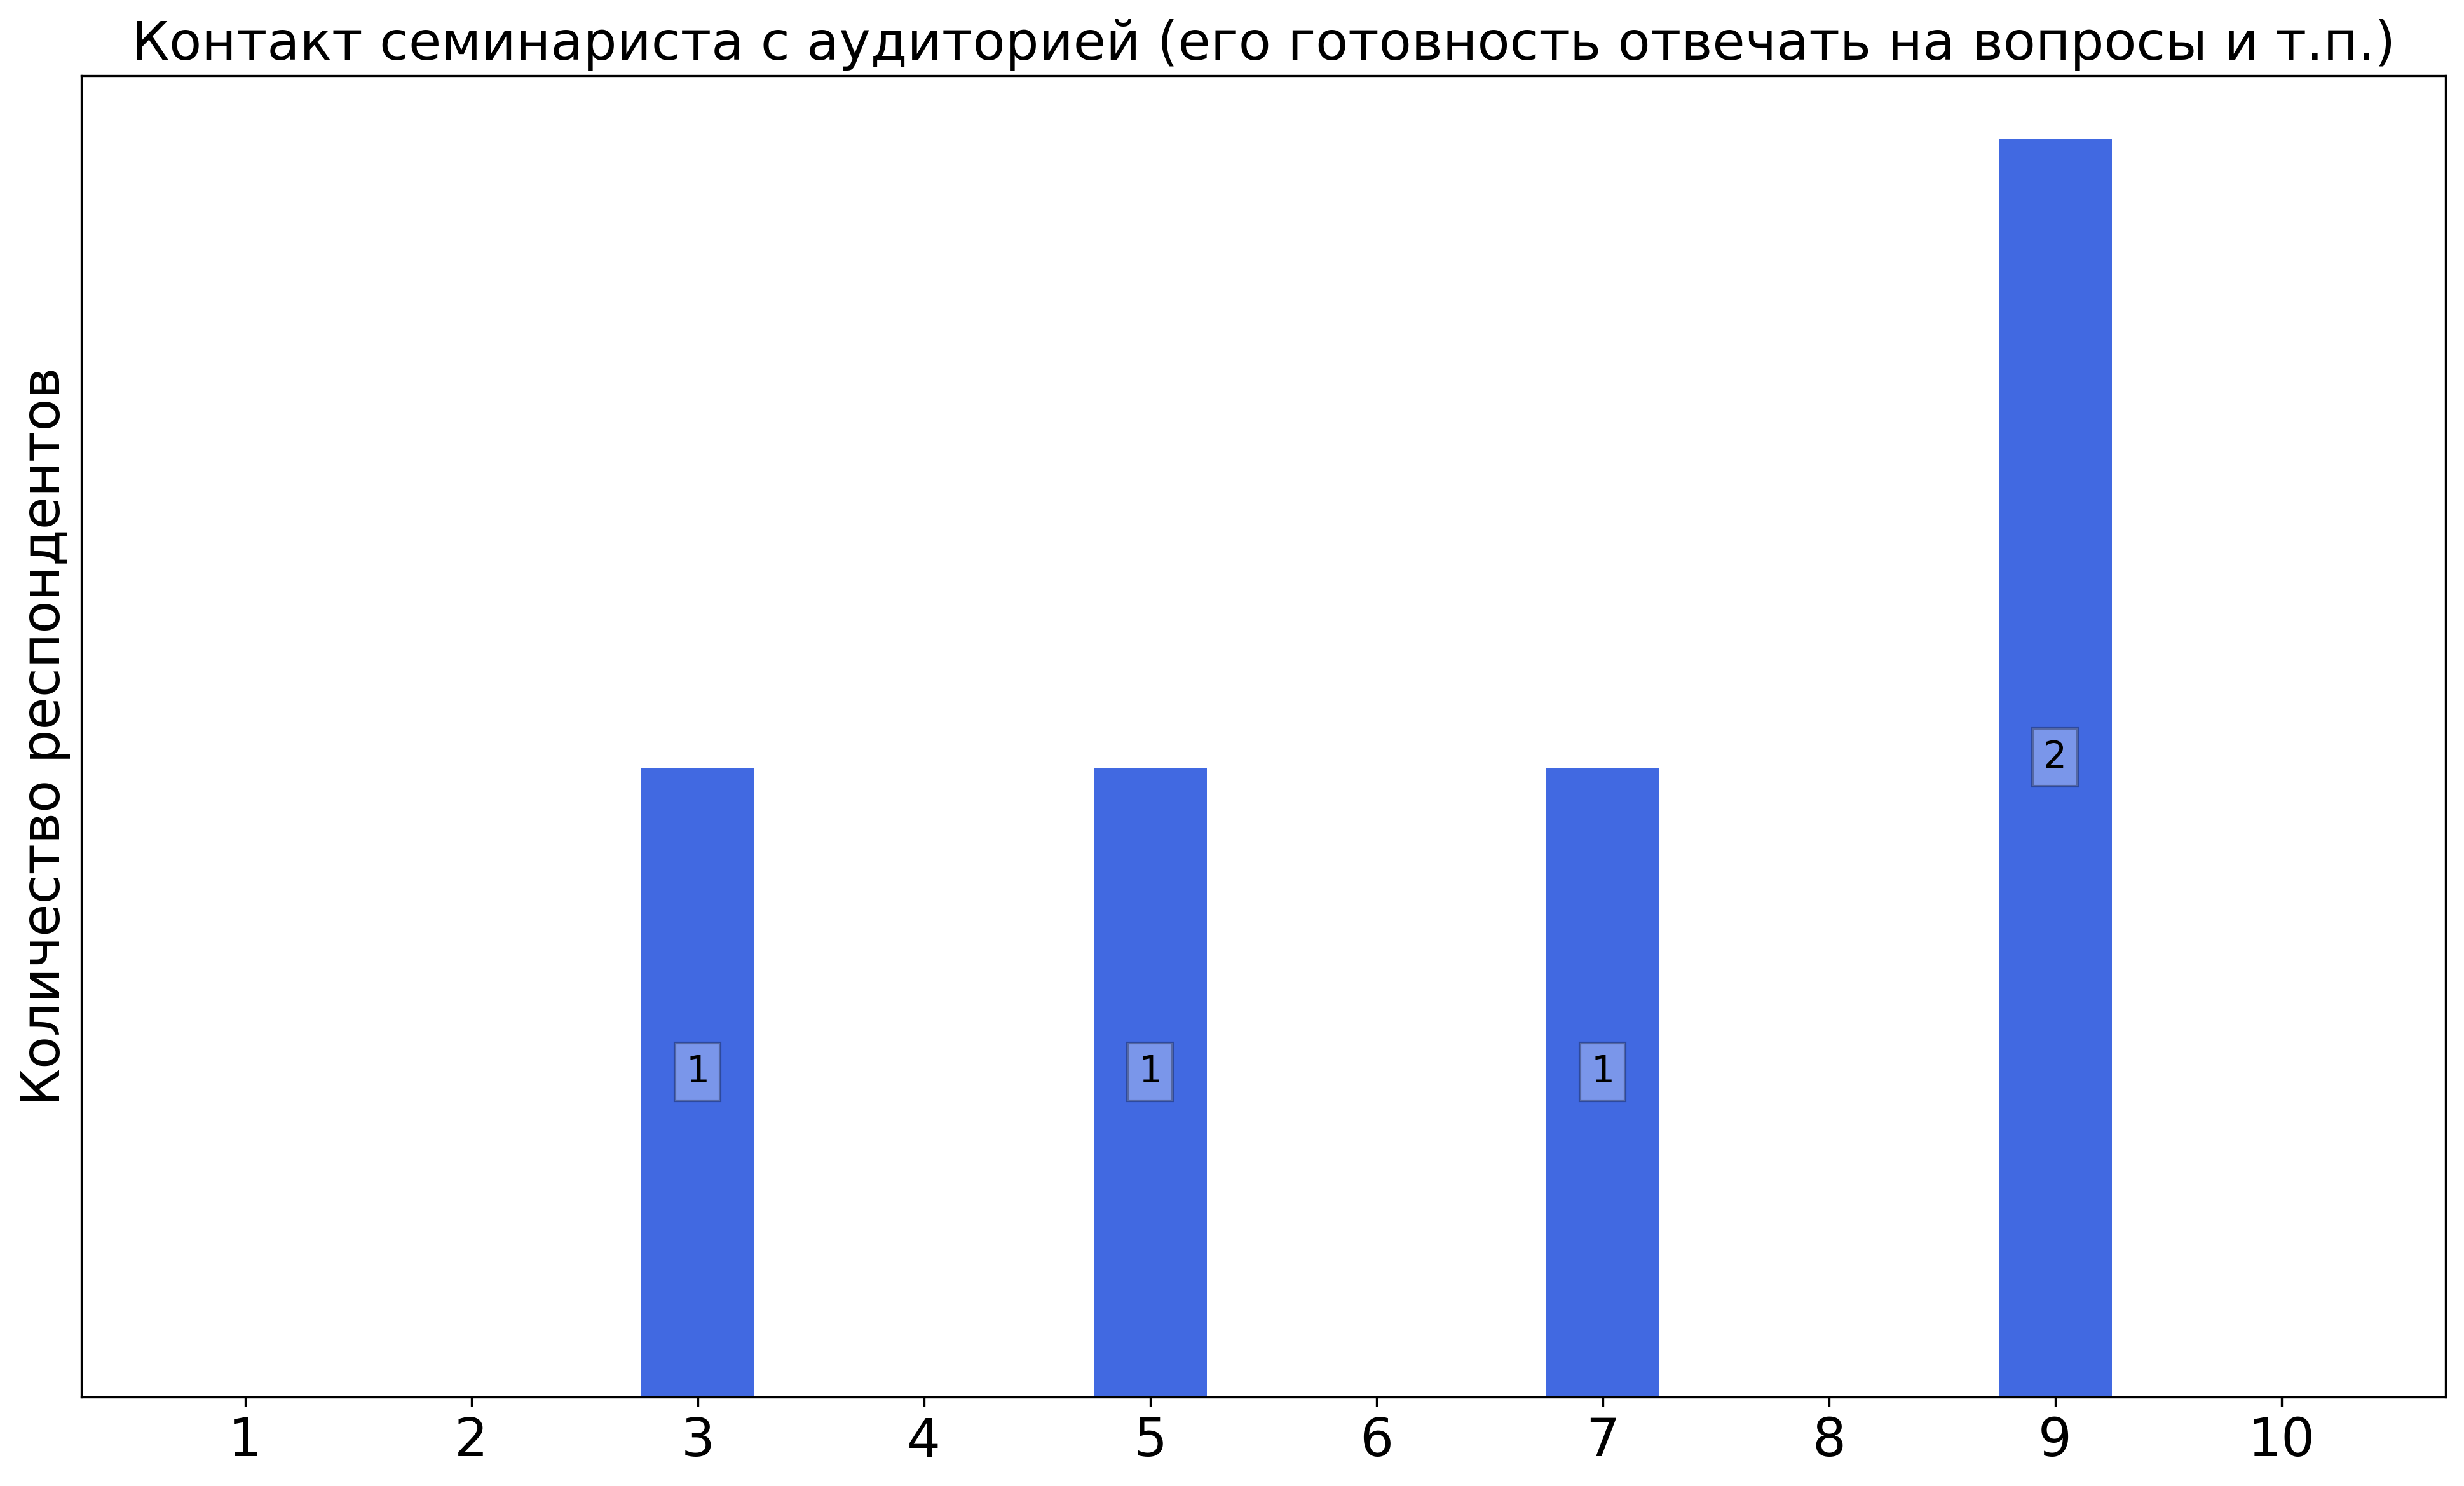
\includegraphics[width=\textwidth]{images/1 course/Дискретный анализ/seminarists-marks-Кириков Е.-0.png}
            \end{subfigure}
            \begin{subfigure}[b]{0.45\textwidth}
                \centering
                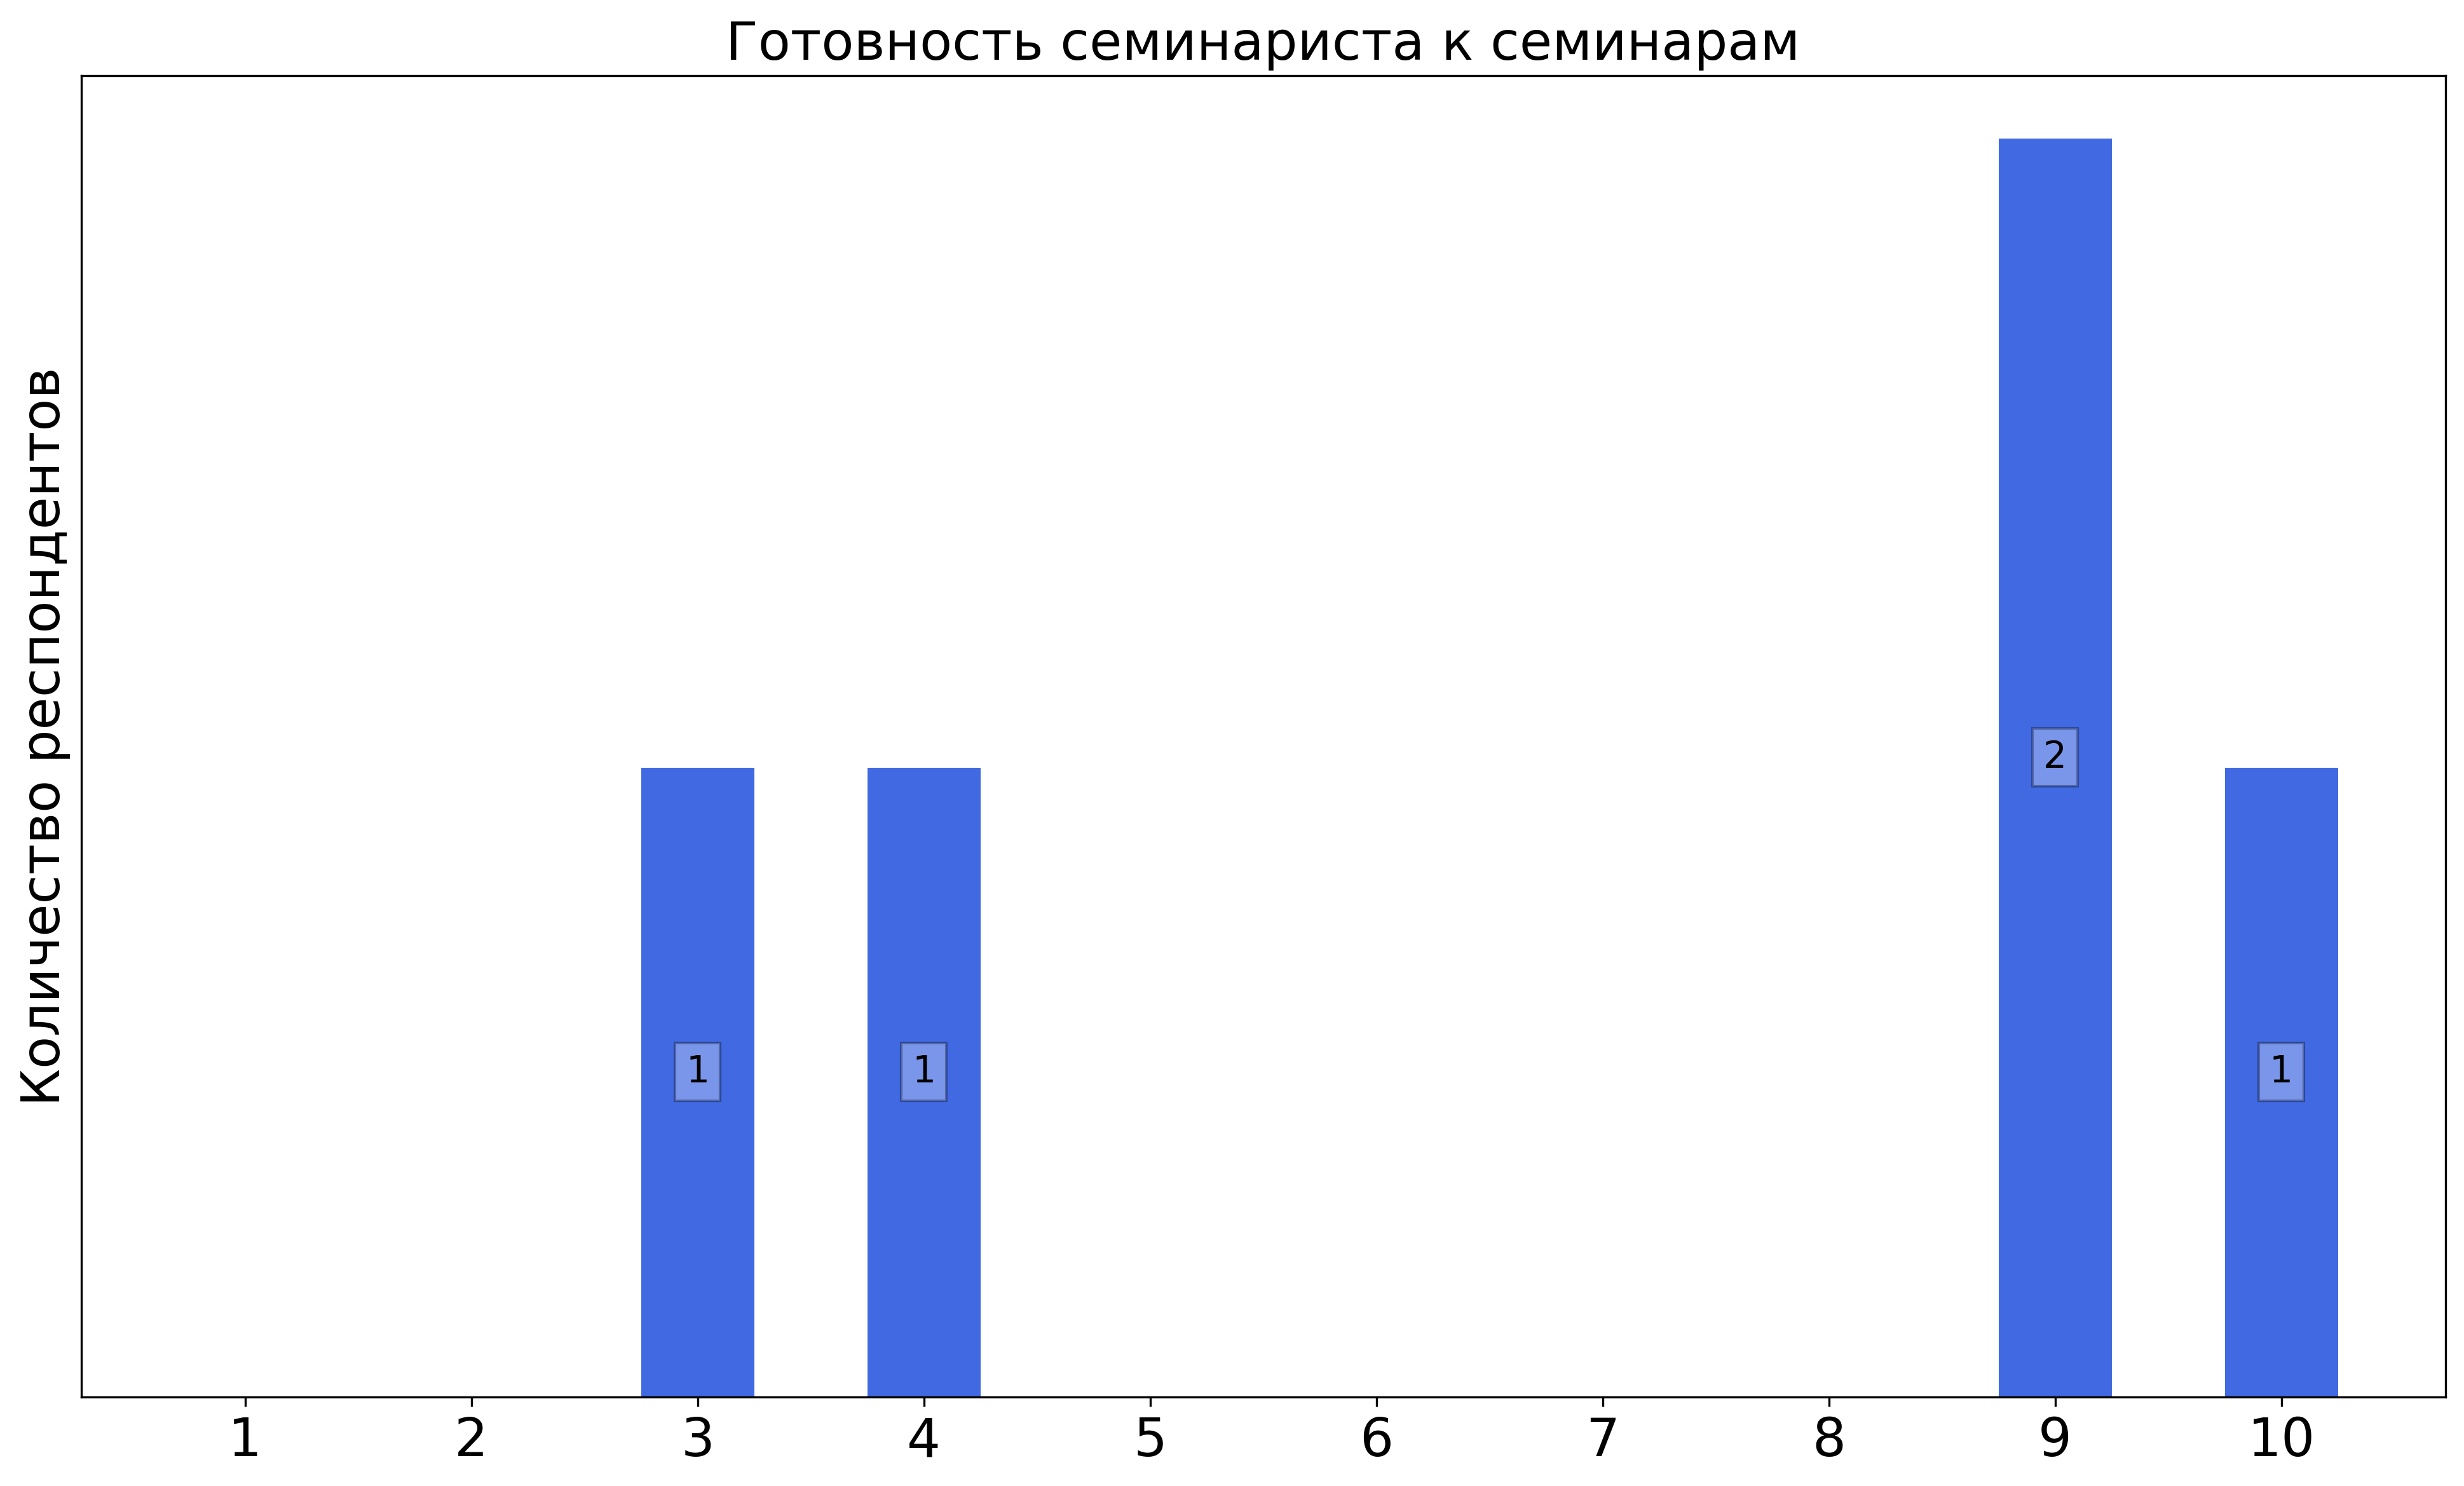
\includegraphics[width=\textwidth]{images/1 course/Дискретный анализ/seminarists-marks-Кириков Е.-1.png}
            \end{subfigure}
            \begin{subfigure}[b]{0.45\textwidth}
                \centering
                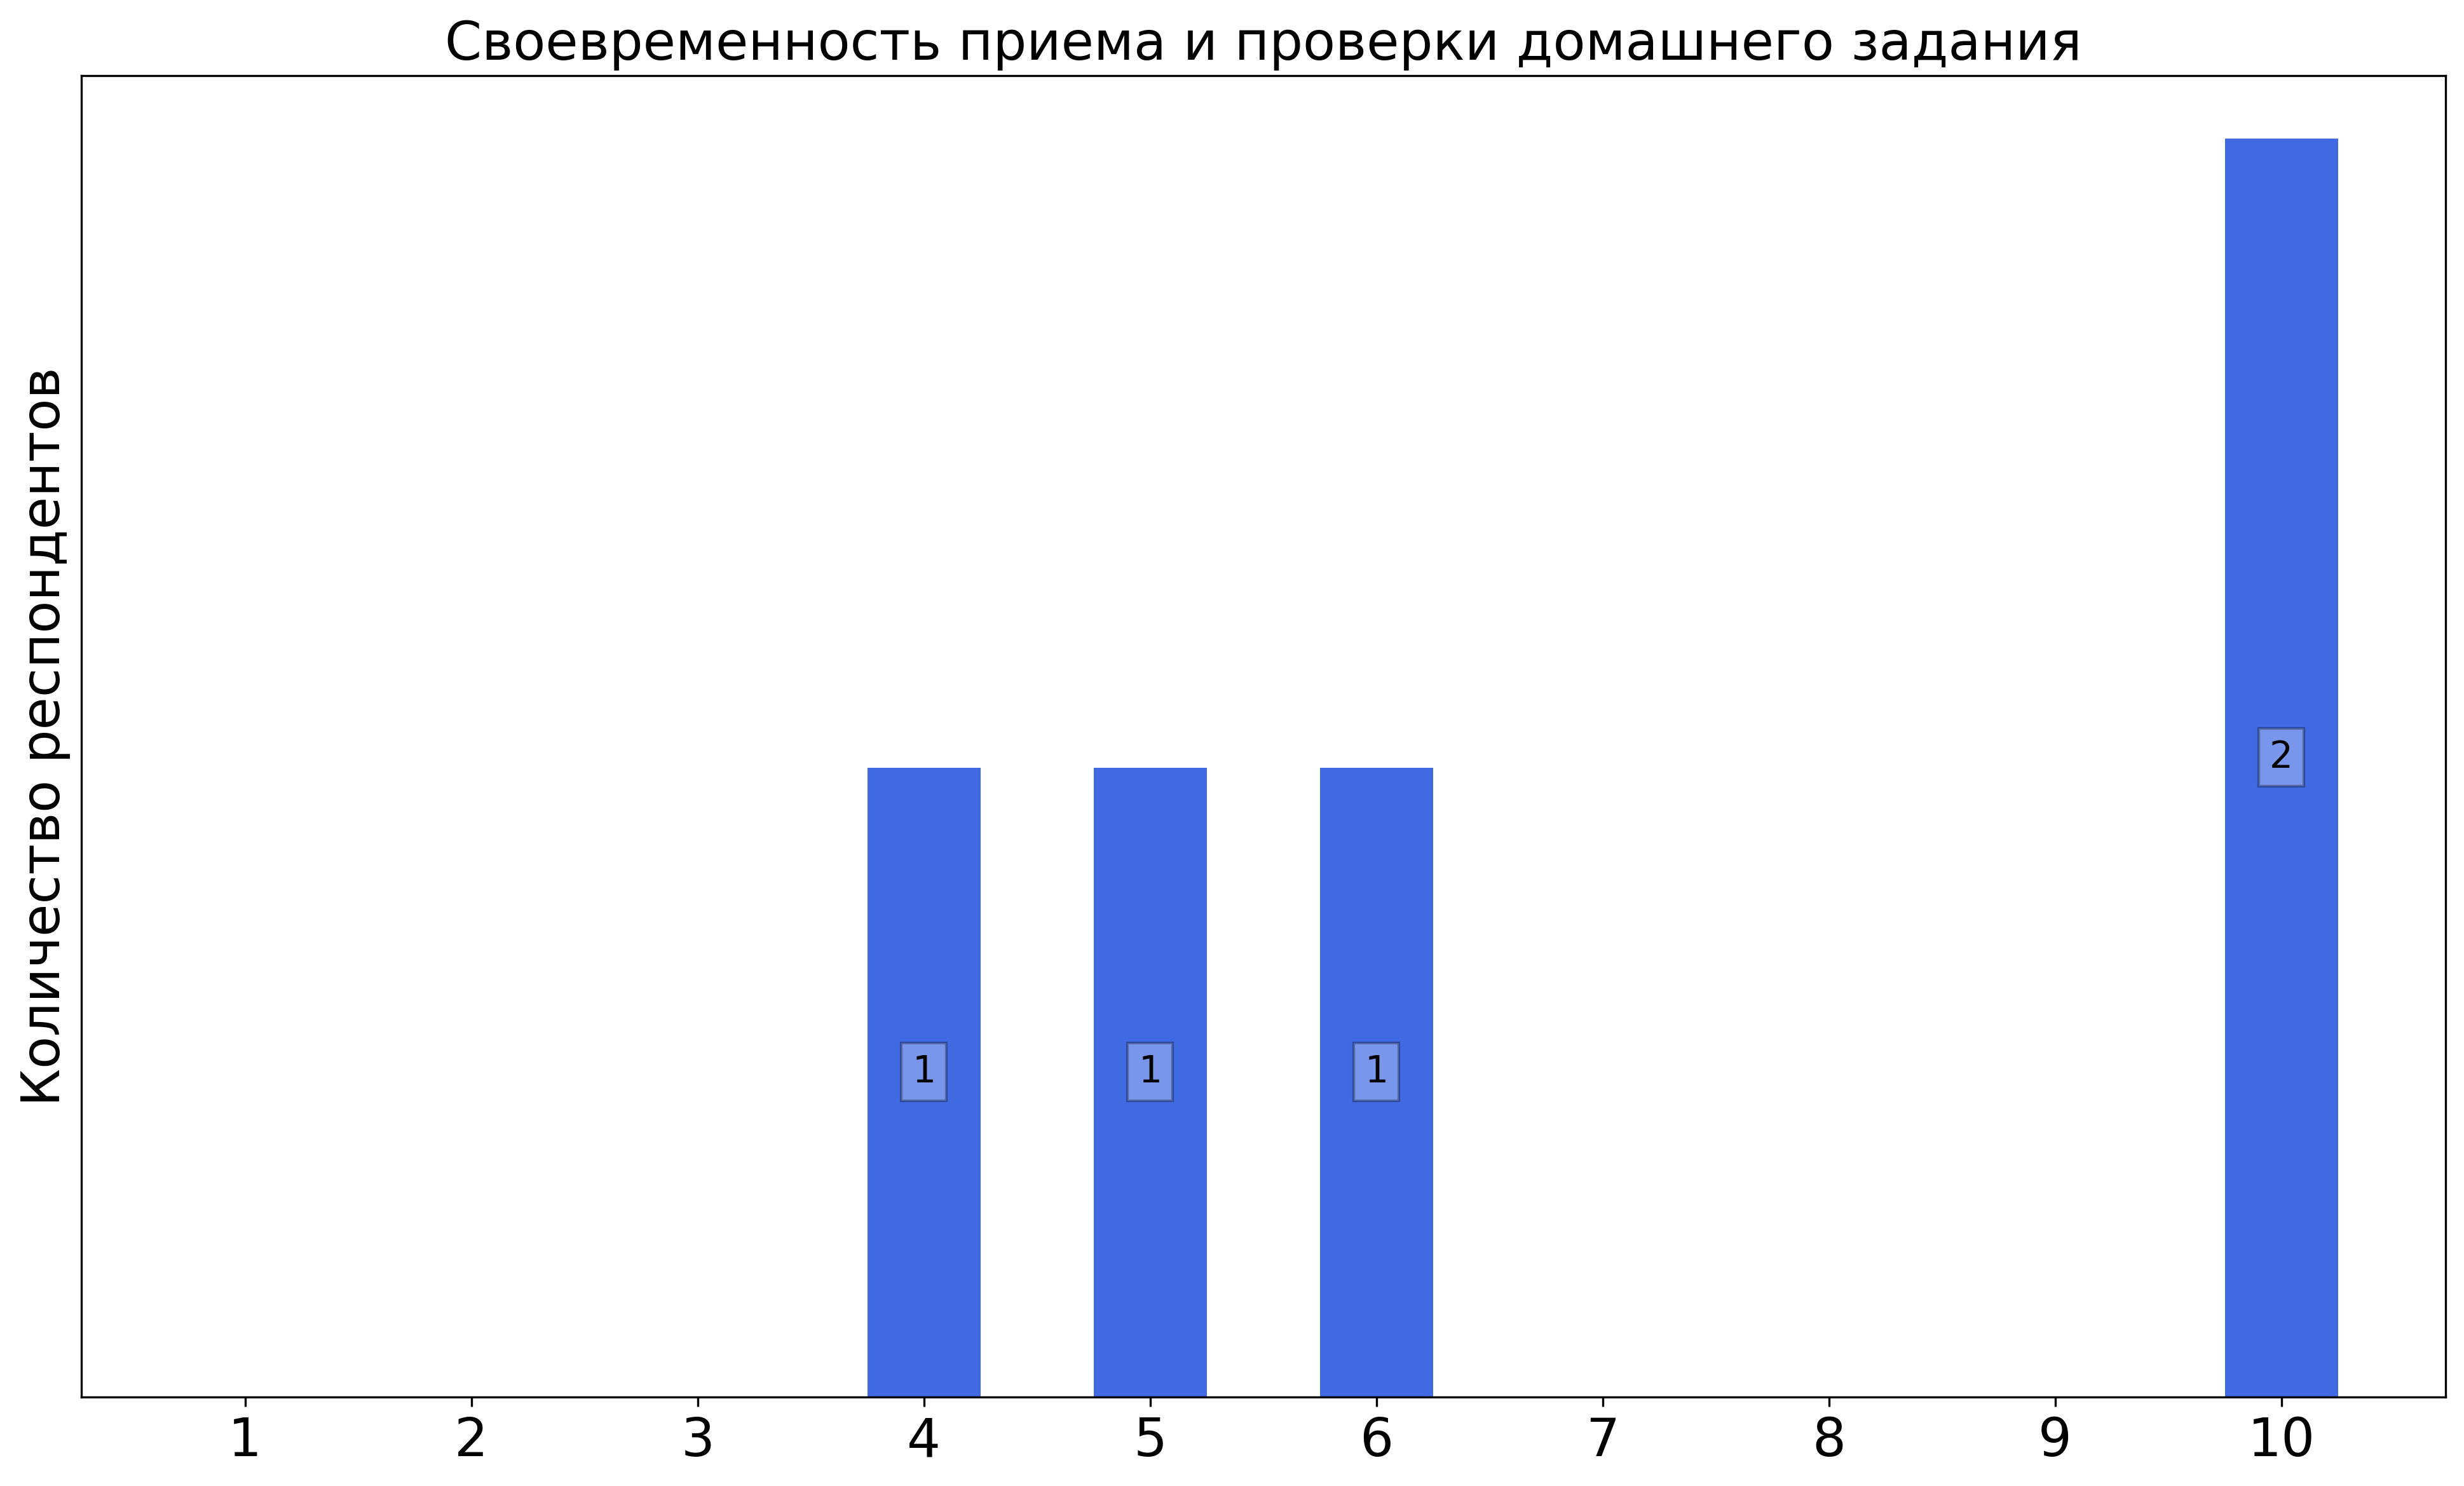
\includegraphics[width=\textwidth]{images/1 course/Дискретный анализ/seminarists-marks-Кириков Е.-2.png}
            \end{subfigure}
            \begin{subfigure}[b]{0.45\textwidth}
                \centering
                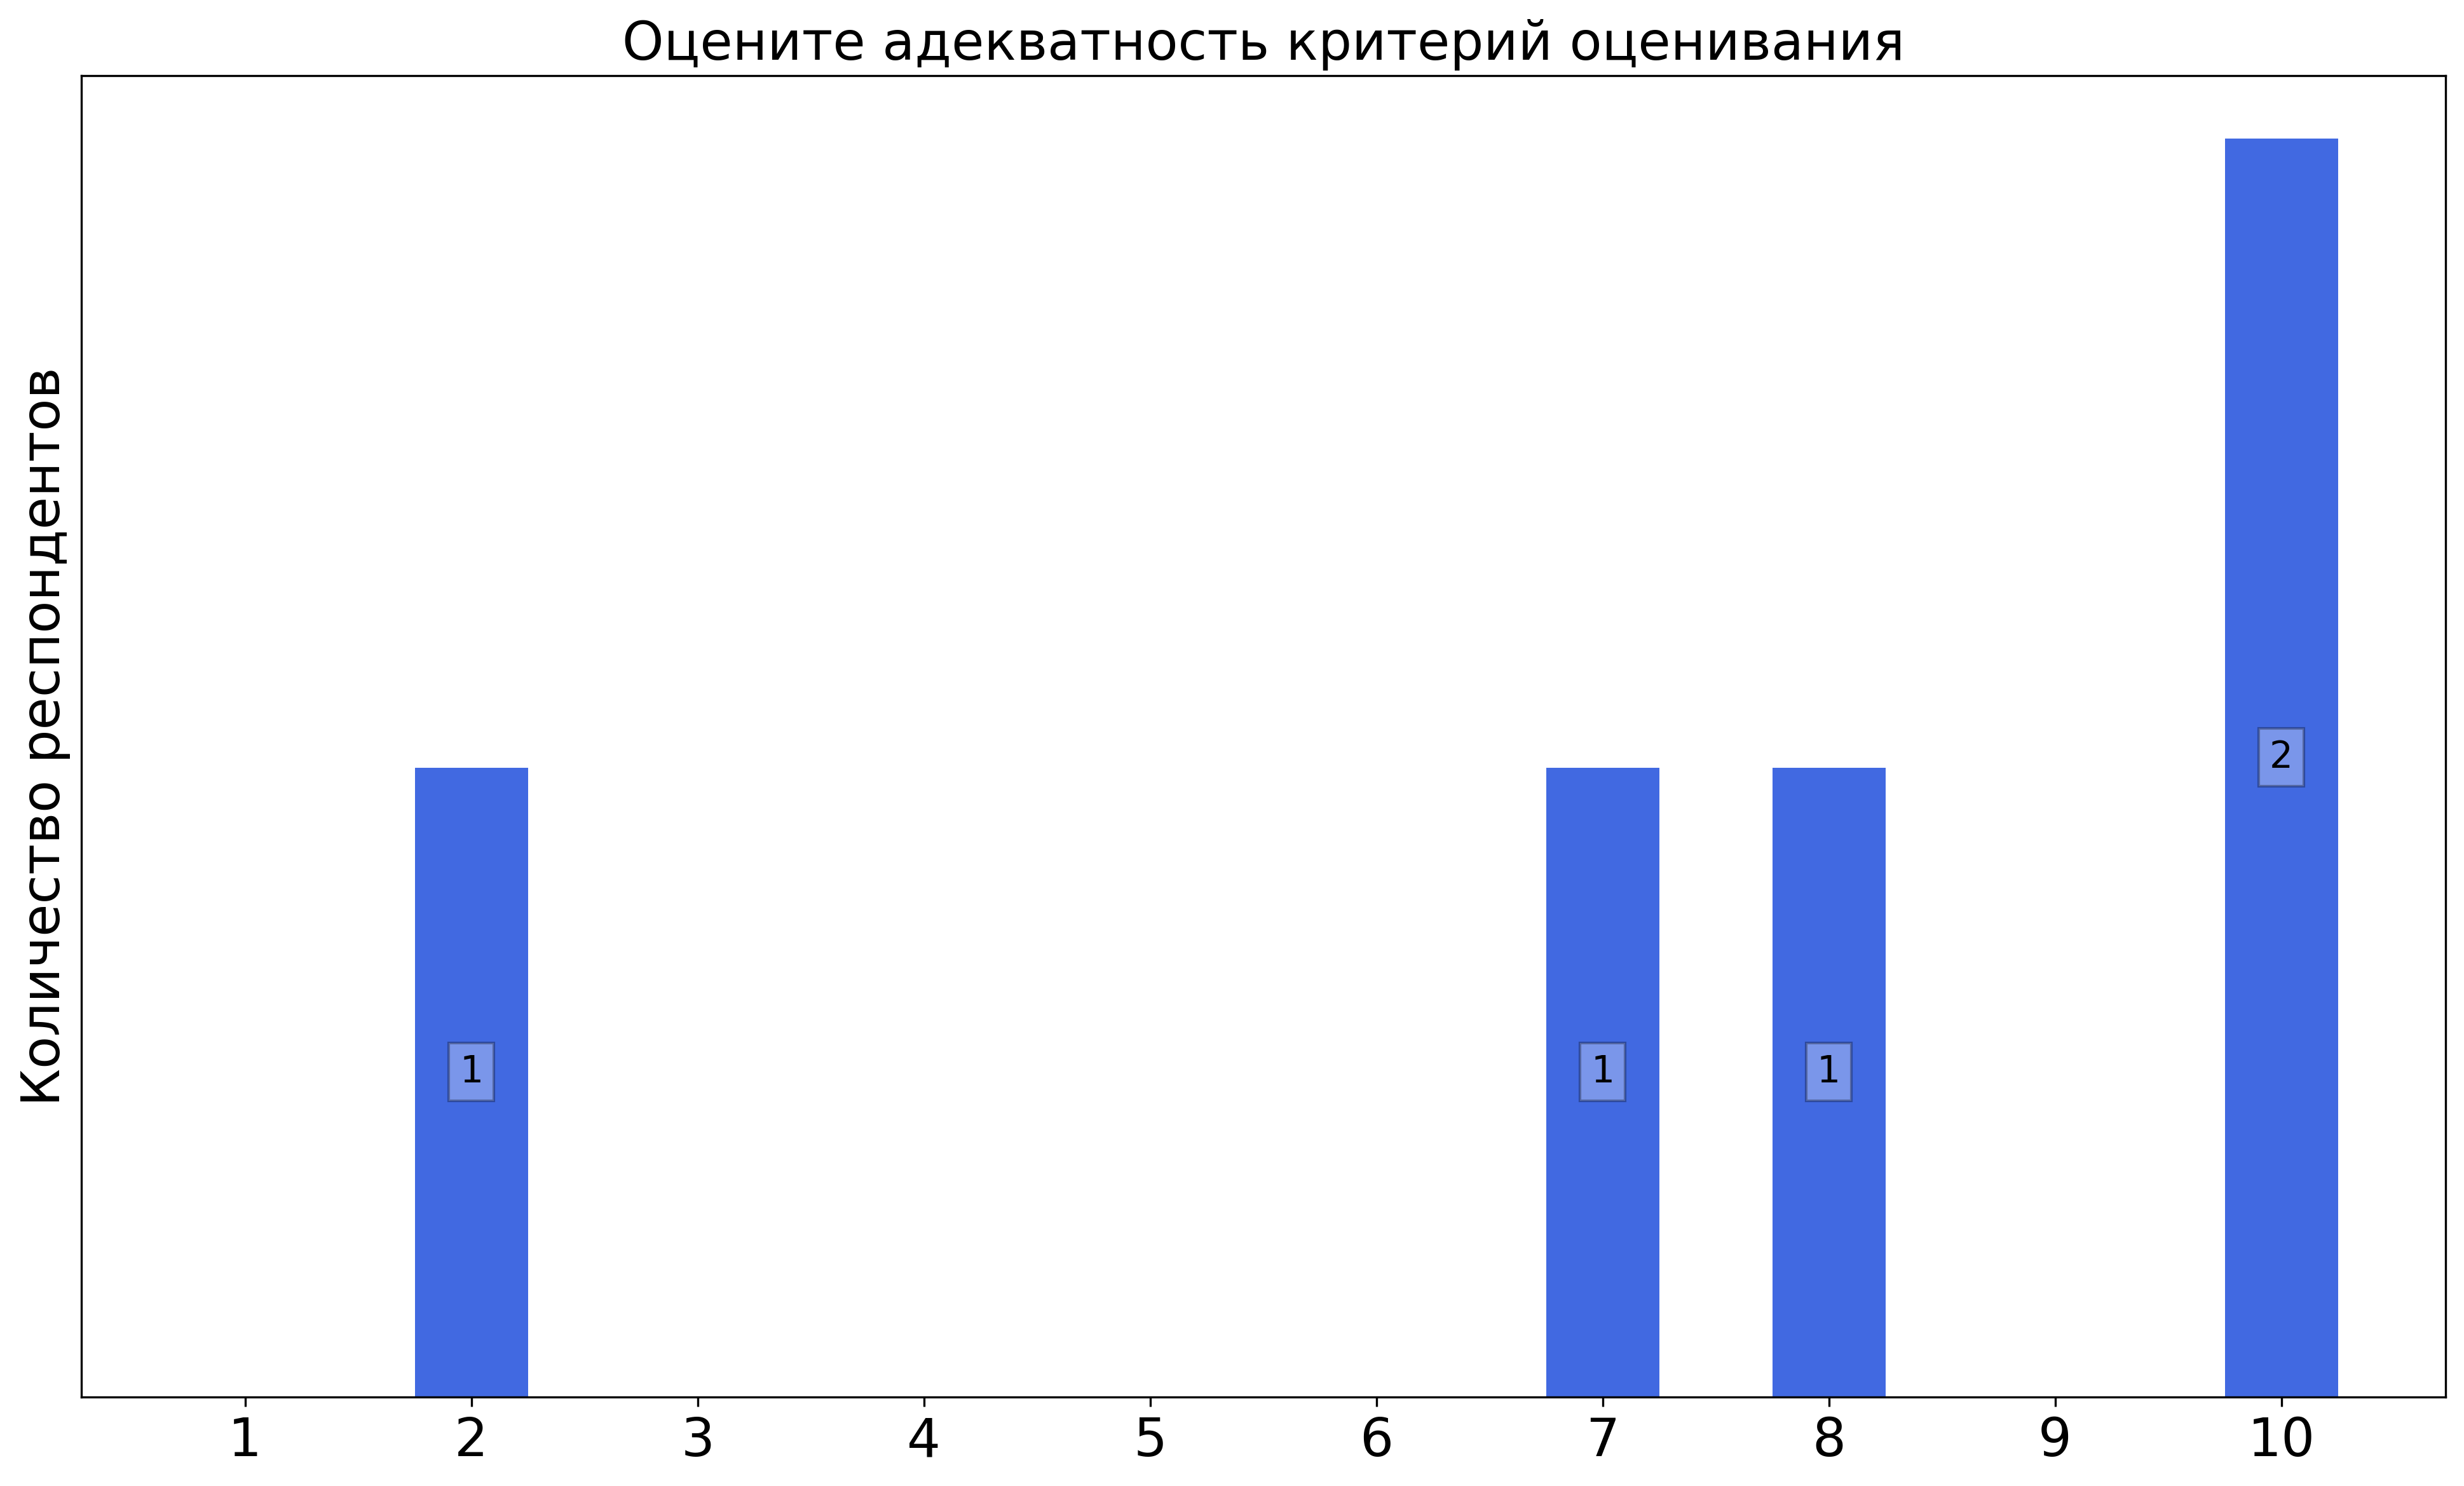
\includegraphics[width=\textwidth]{images/1 course/Дискретный анализ/seminarists-marks-Кириков Е.-3.png}
            \end{subfigure}	
            \caption{Оценки респондентов о качестве преподавания семинаров}
        \end{figure}

    \subsubsection{Отзыв студентов о семинарах. Семинарист: Плетнёв Н.В.}
		\begin{figure}[H]
			\centering
			\begin{subfigure}[b]{0.45\textwidth}
				\centering
				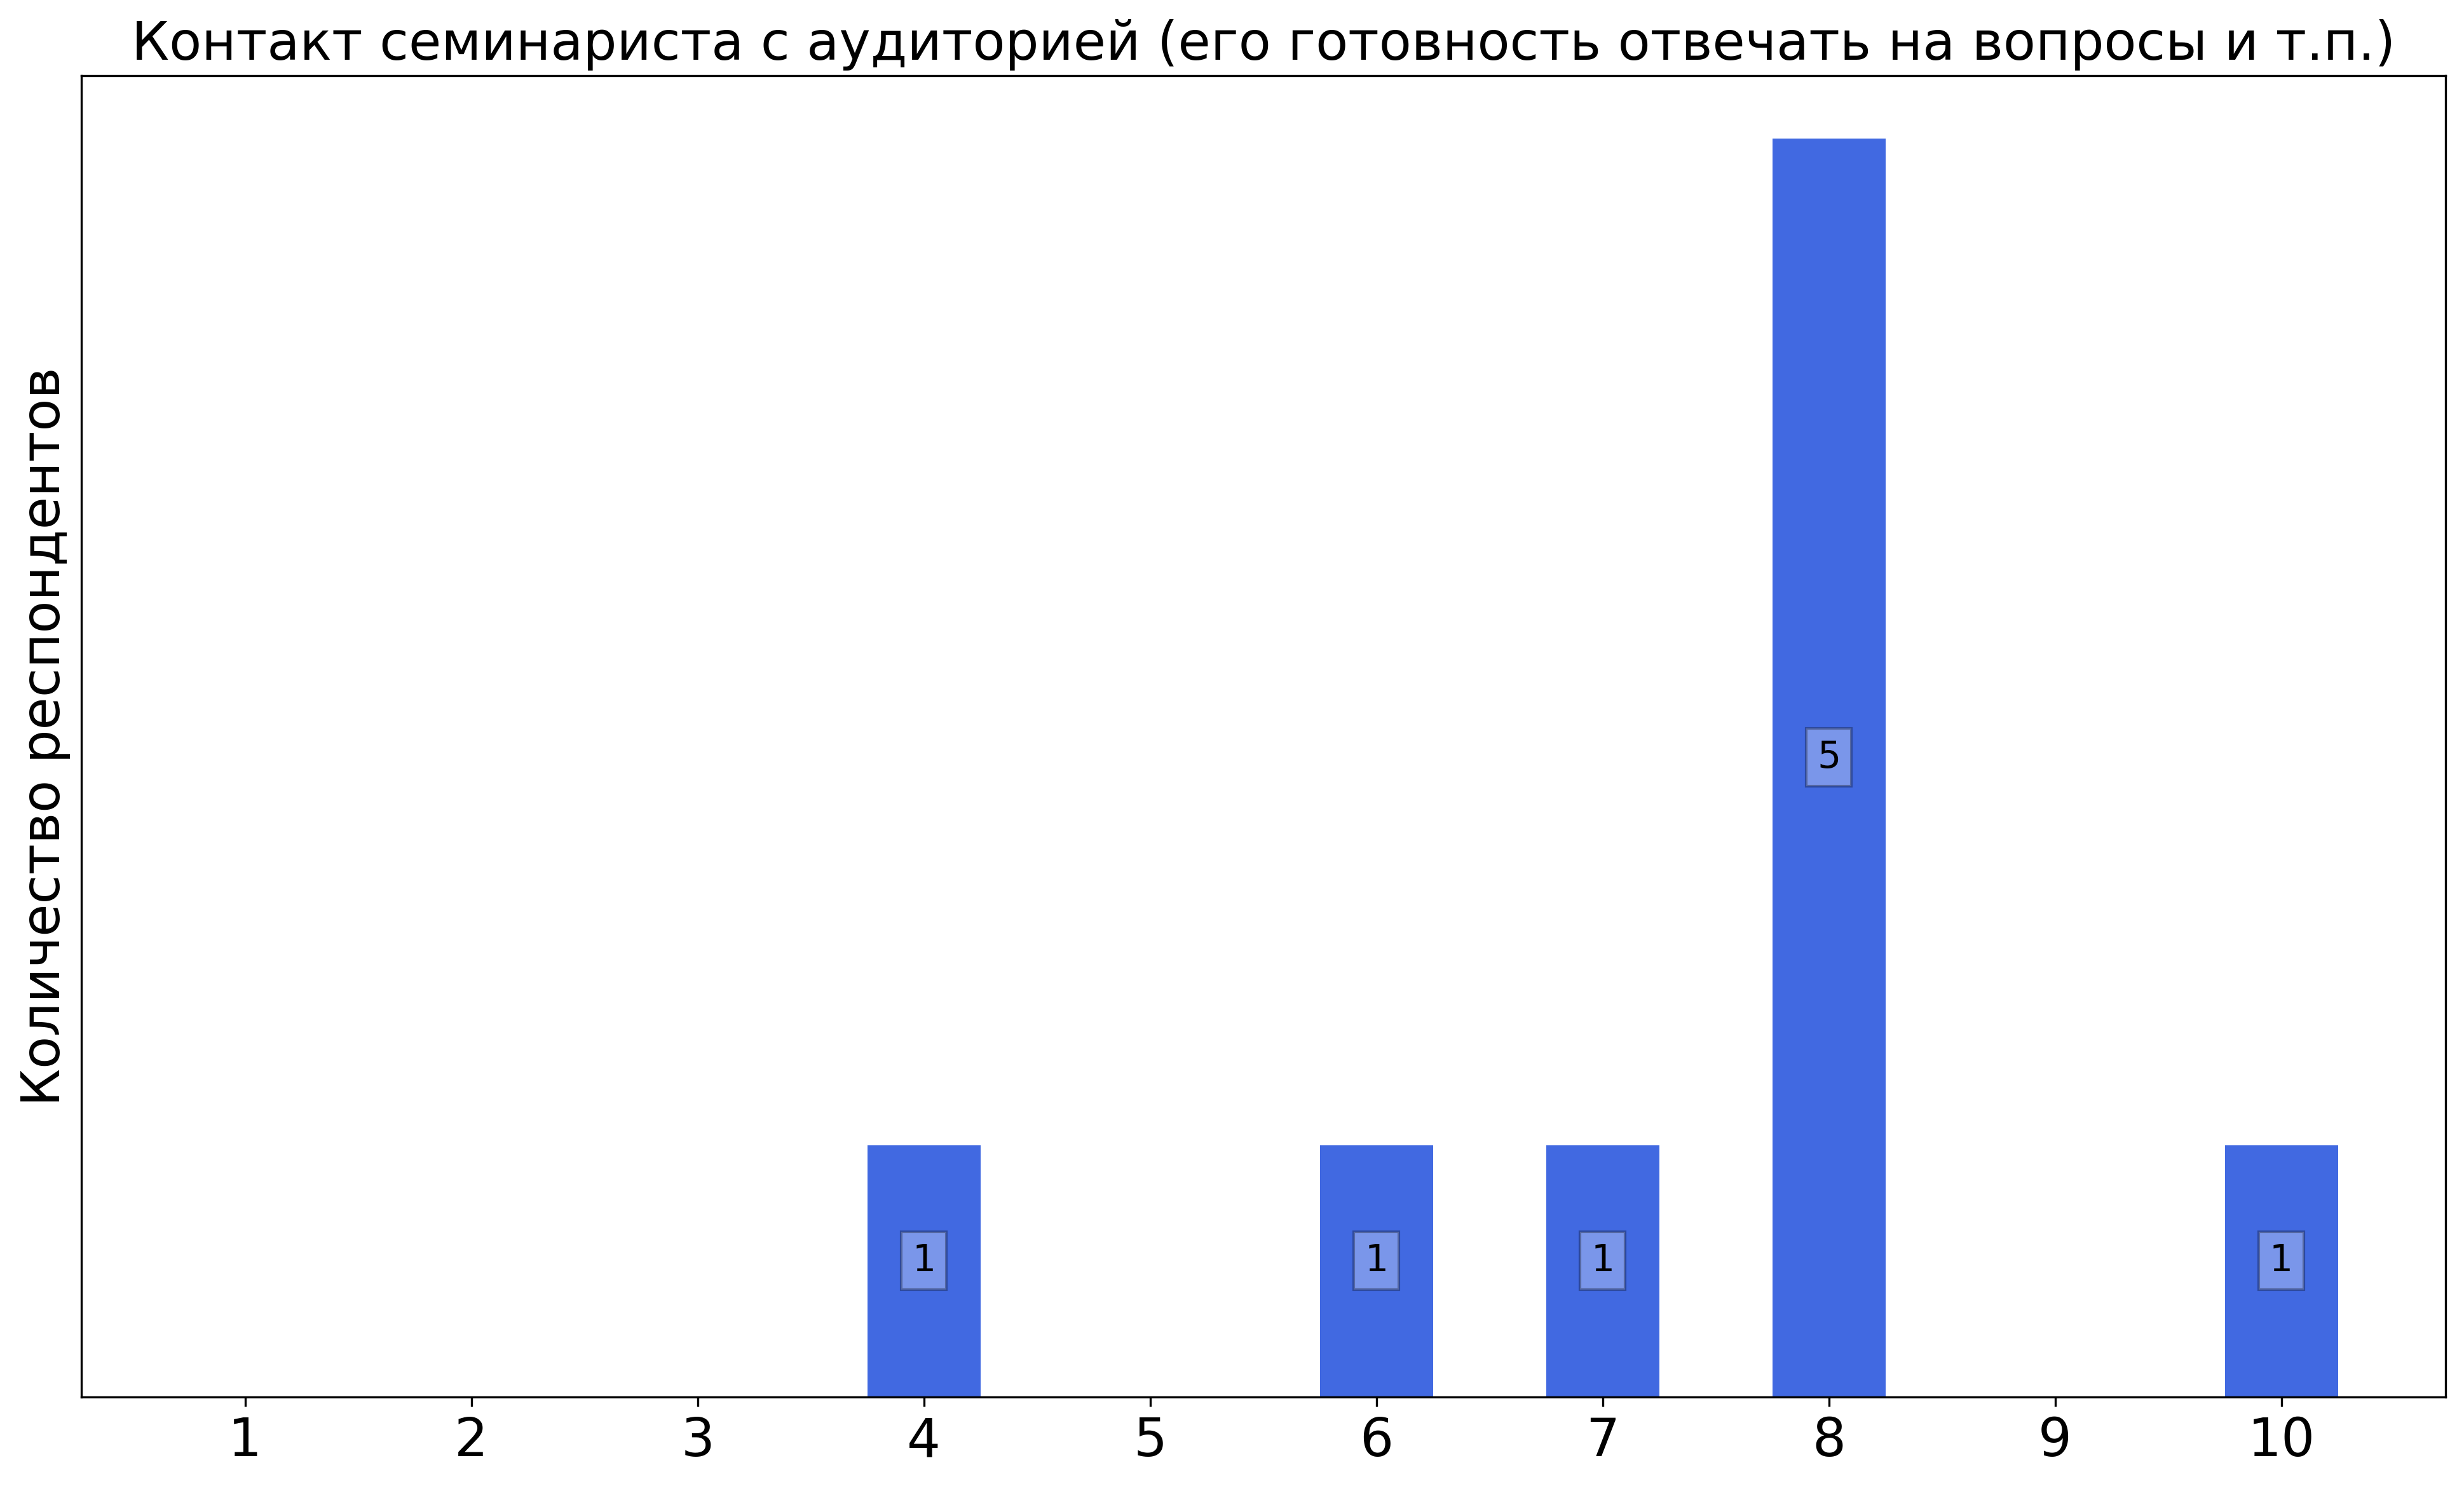
\includegraphics[width=\textwidth]{images/1 course/Дискретный анализ/seminarists-marks-Плетнёв Н.В.-0.png}
			\end{subfigure}
			\begin{subfigure}[b]{0.45\textwidth}
				\centering
				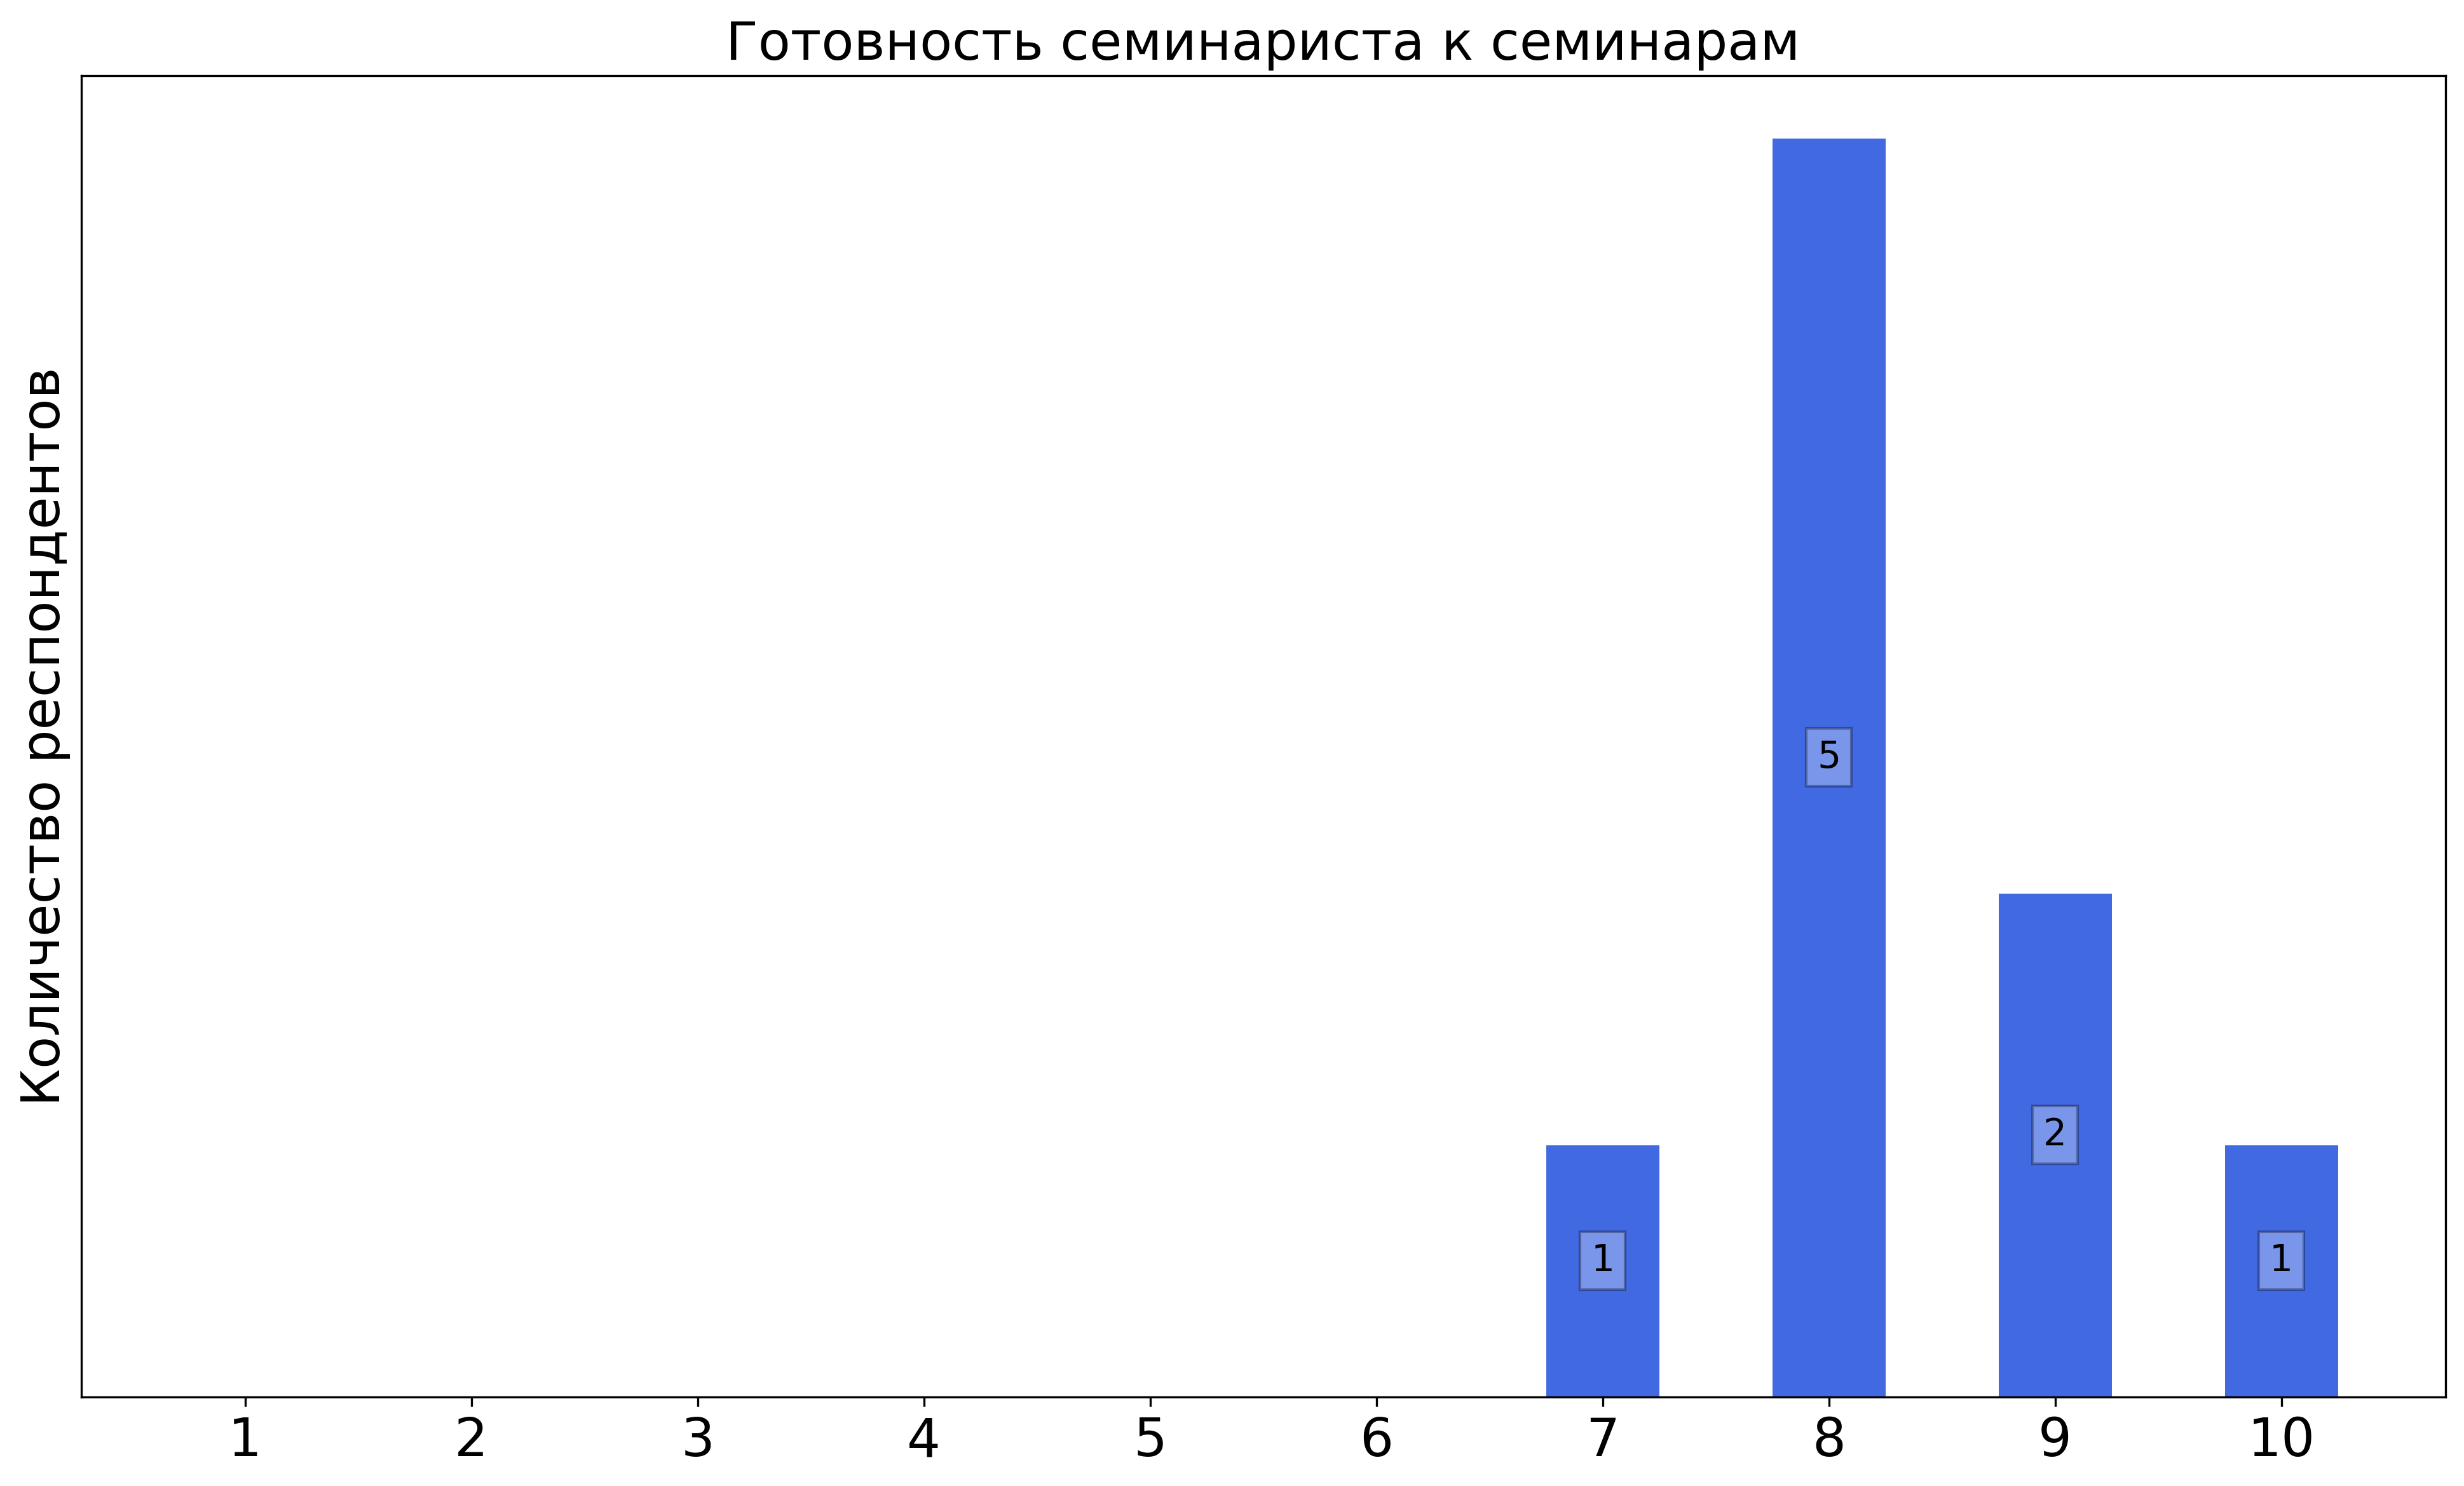
\includegraphics[width=\textwidth]{images/1 course/Дискретный анализ/seminarists-marks-Плетнёв Н.В.-1.png}
			\end{subfigure}
			\begin{subfigure}[b]{0.45\textwidth}
				\centering
				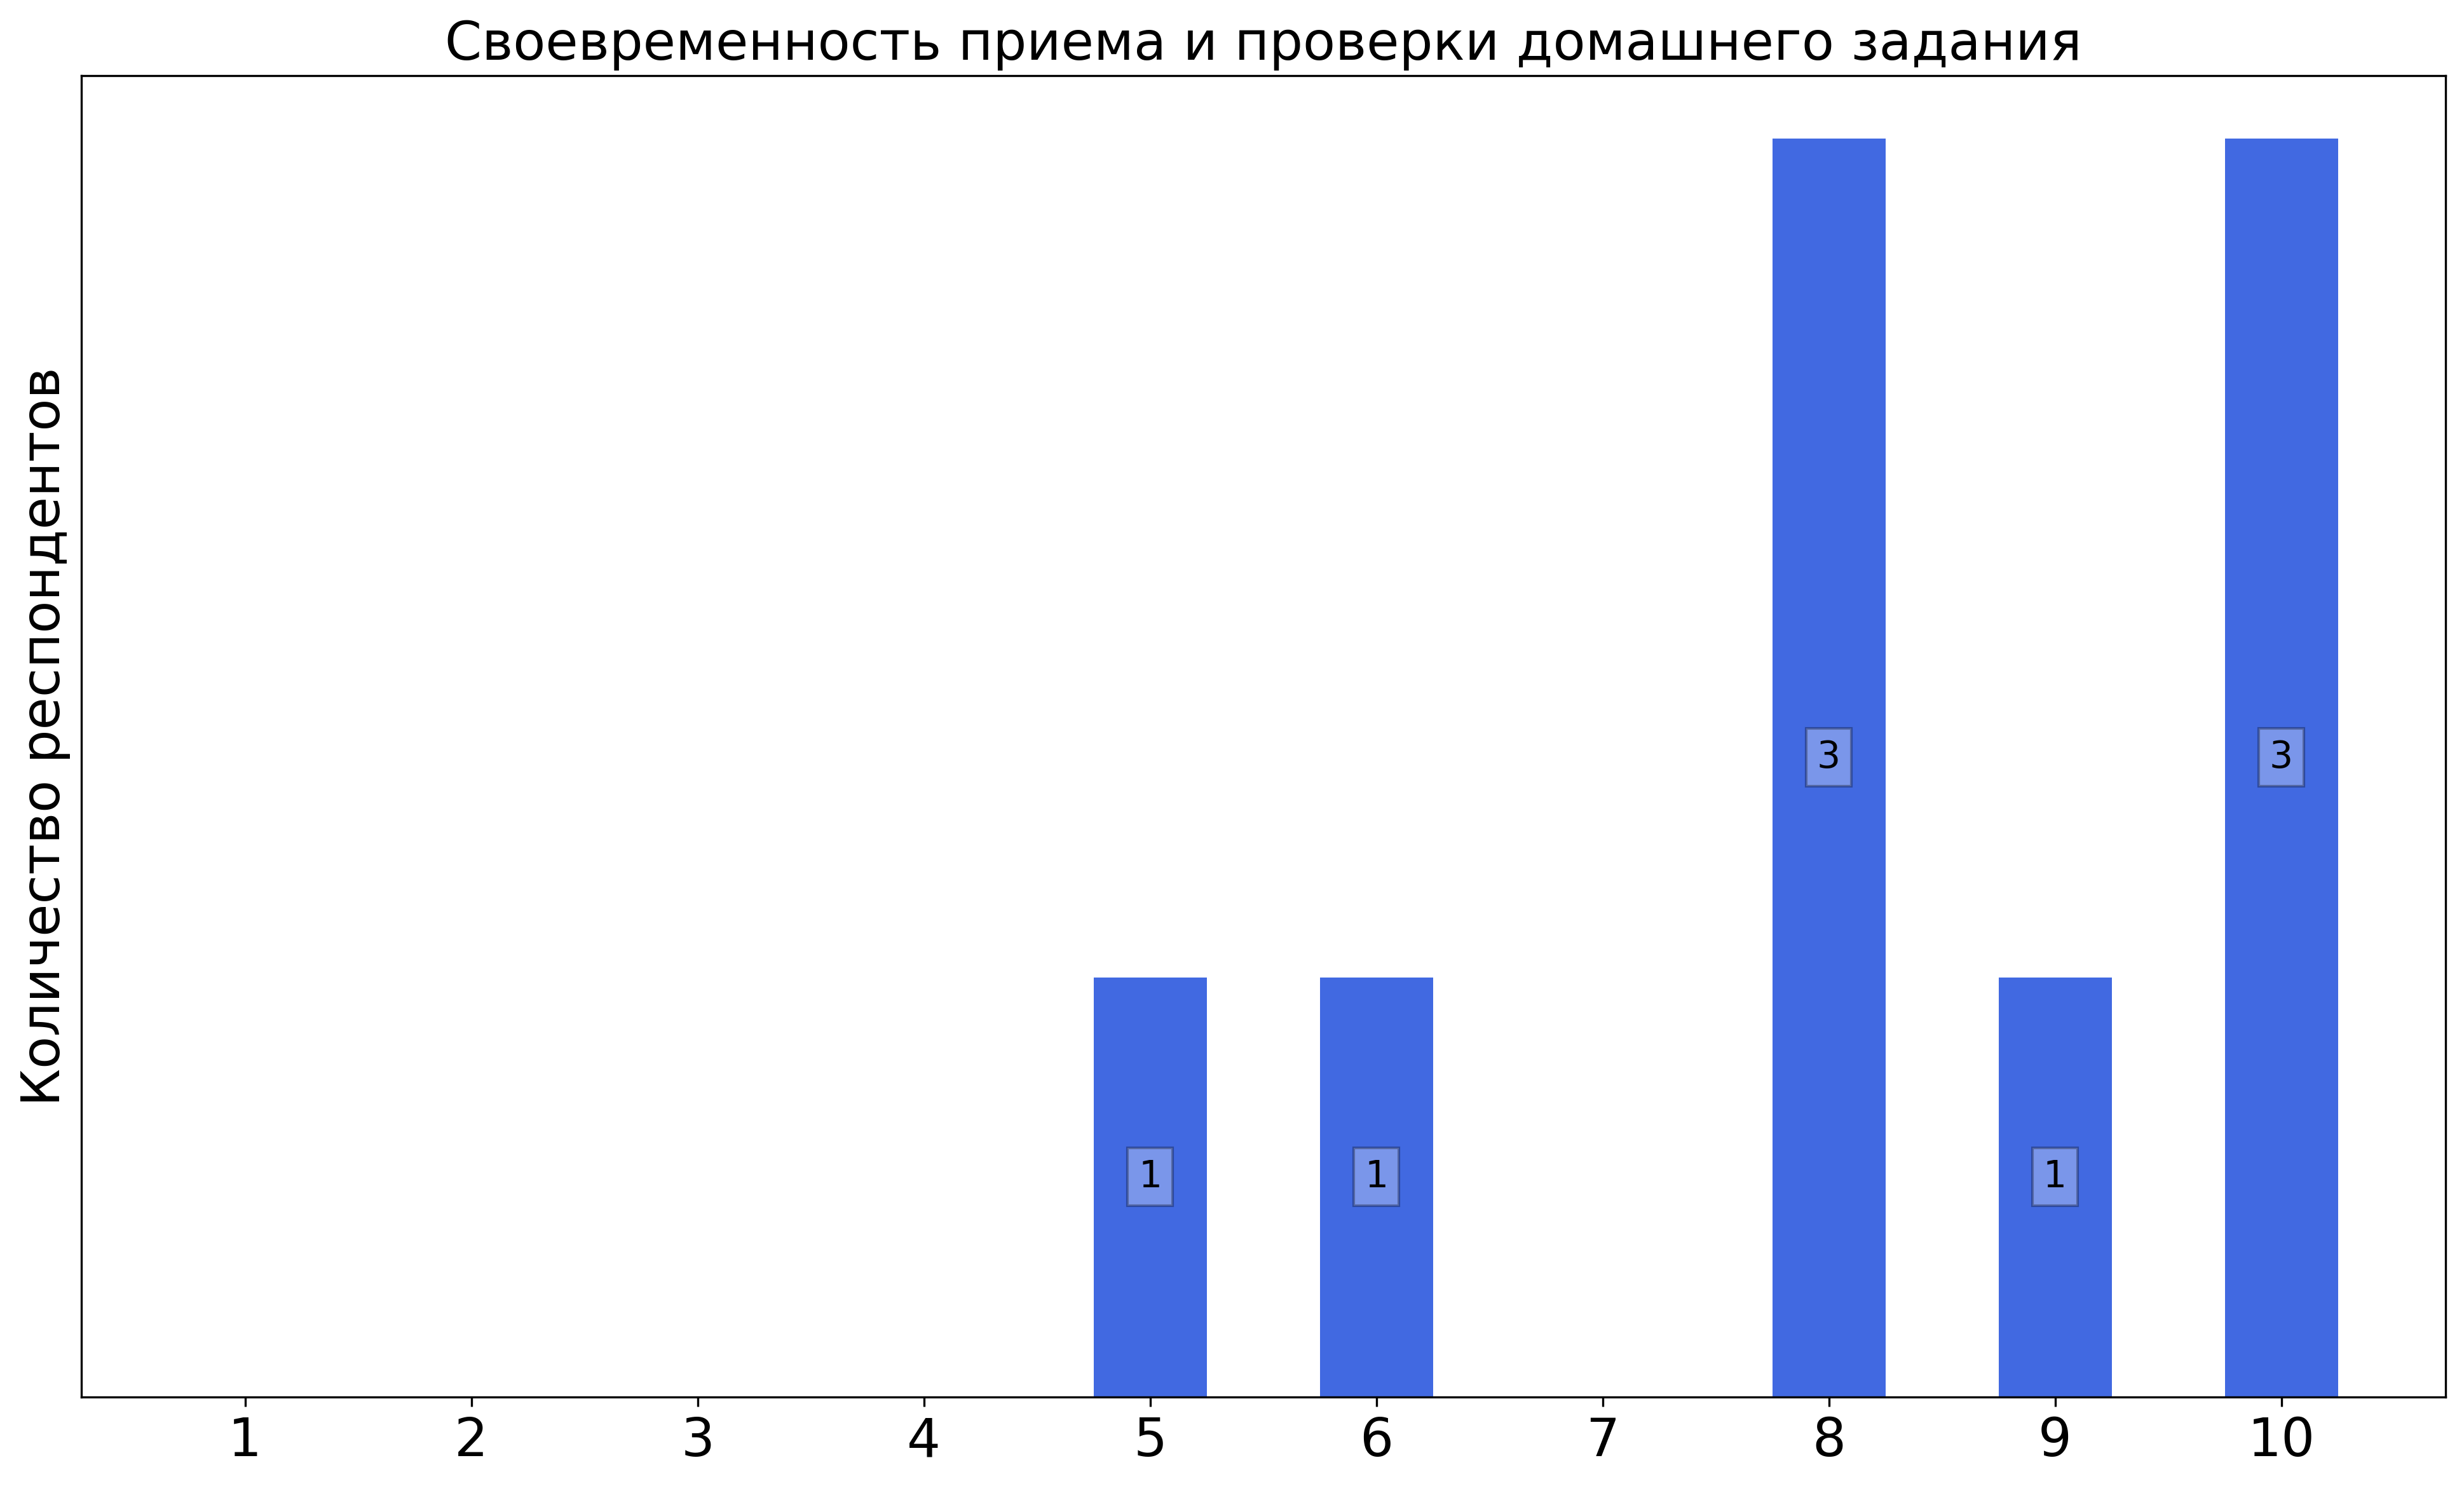
\includegraphics[width=\textwidth]{images/1 course/Дискретный анализ/seminarists-marks-Плетнёв Н.В.-2.png}
			\end{subfigure}
			\begin{subfigure}[b]{0.45\textwidth}
				\centering
				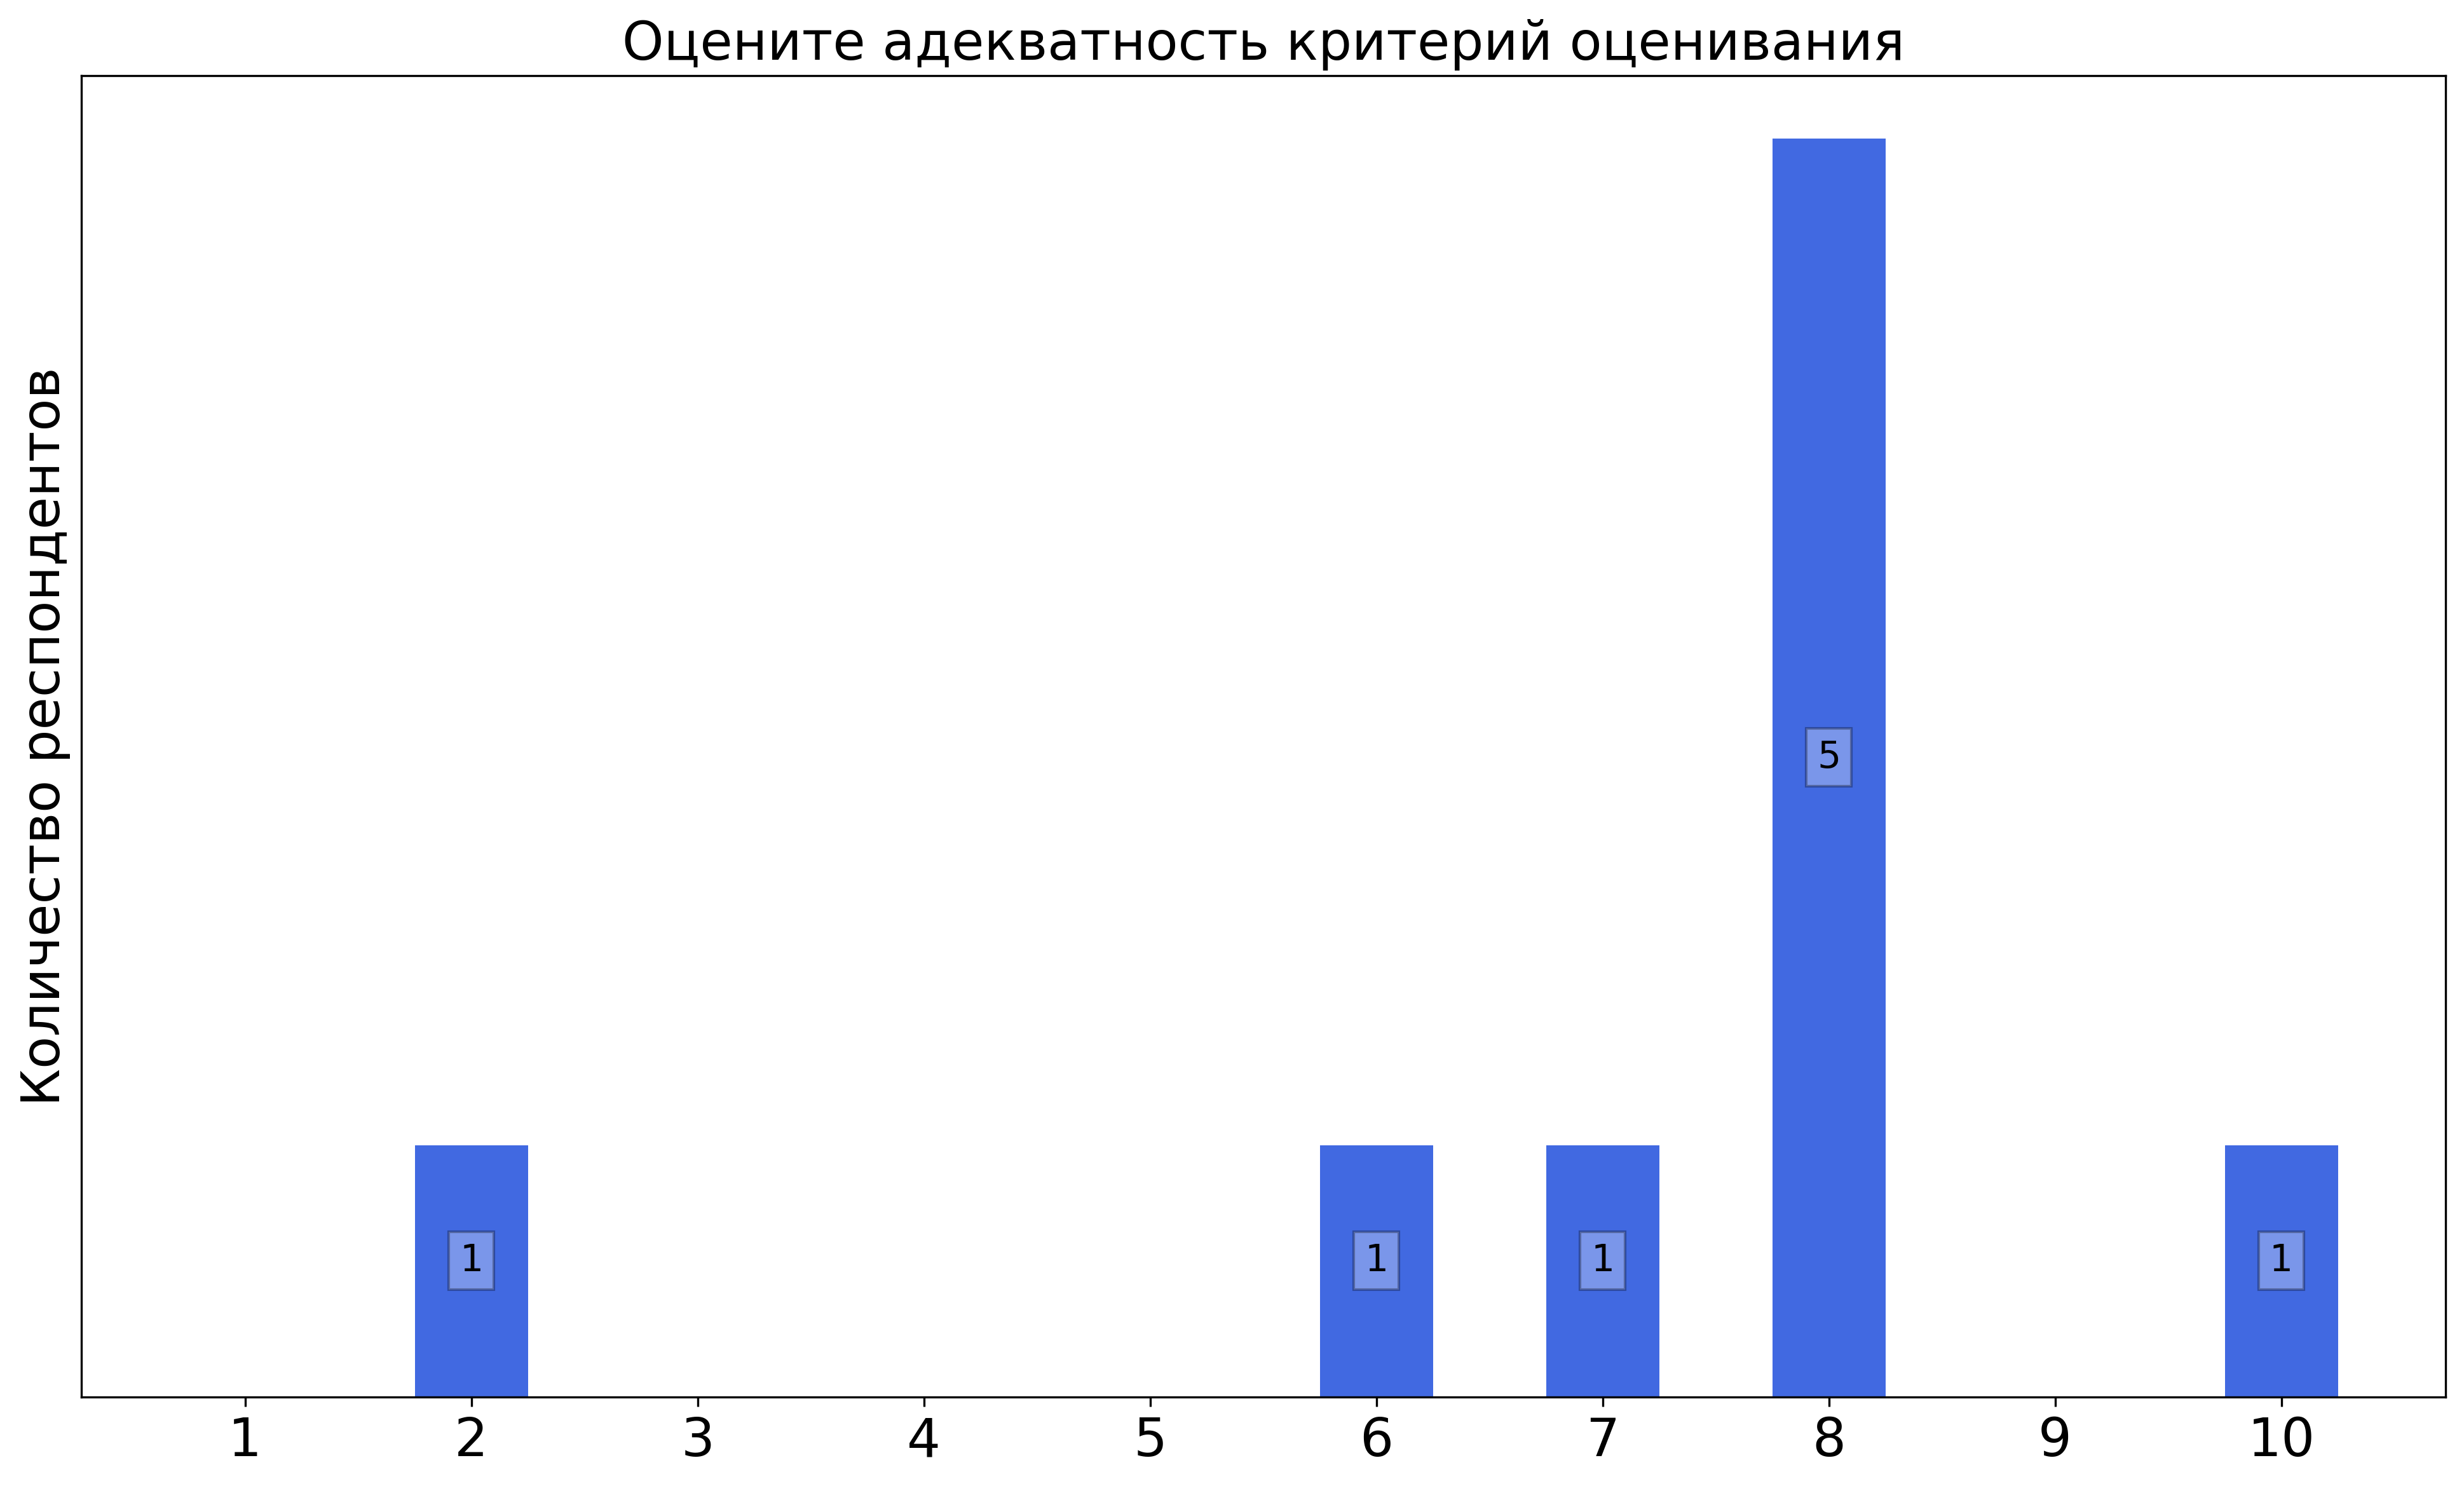
\includegraphics[width=\textwidth]{images/1 course/Дискретный анализ/seminarists-marks-Плетнёв Н.В.-3.png}
			\end{subfigure}	
			\caption{Оценки респондентов о качестве преподавания семинаров}
		\end{figure}

		\textbf{Комментарии студентов о семинаристе\protect\footnote{сохранены оригинальные орфография и пунктуация}}
            \begin{commentbox} 
                он, в целом, халява, просто всех пугает, но в конце семестра надо зазубрить теорию/списать его работу 
            \end{commentbox} 
        
            \begin{commentbox} 
                хороший семинарист, реально все знает, каждую задачу понимает и рассказывает. но меня обычно хватало только на половину семинара, дальше я переставал все понимать. Говорят что он факер, но это совсем не так, если правда проявлять интерес к предмету, то на хор можно спокойно рассчитывать, дает сдавать дополнительные задания для повышения оценки.  
            \end{commentbox} 

        
    \subsubsection{Отзыв студентов о семинарах. Семинарист: Табунов А.В.}
        \begin{figure}[H]
            \centering
            \begin{subfigure}[b]{0.45\textwidth}
                \centering
                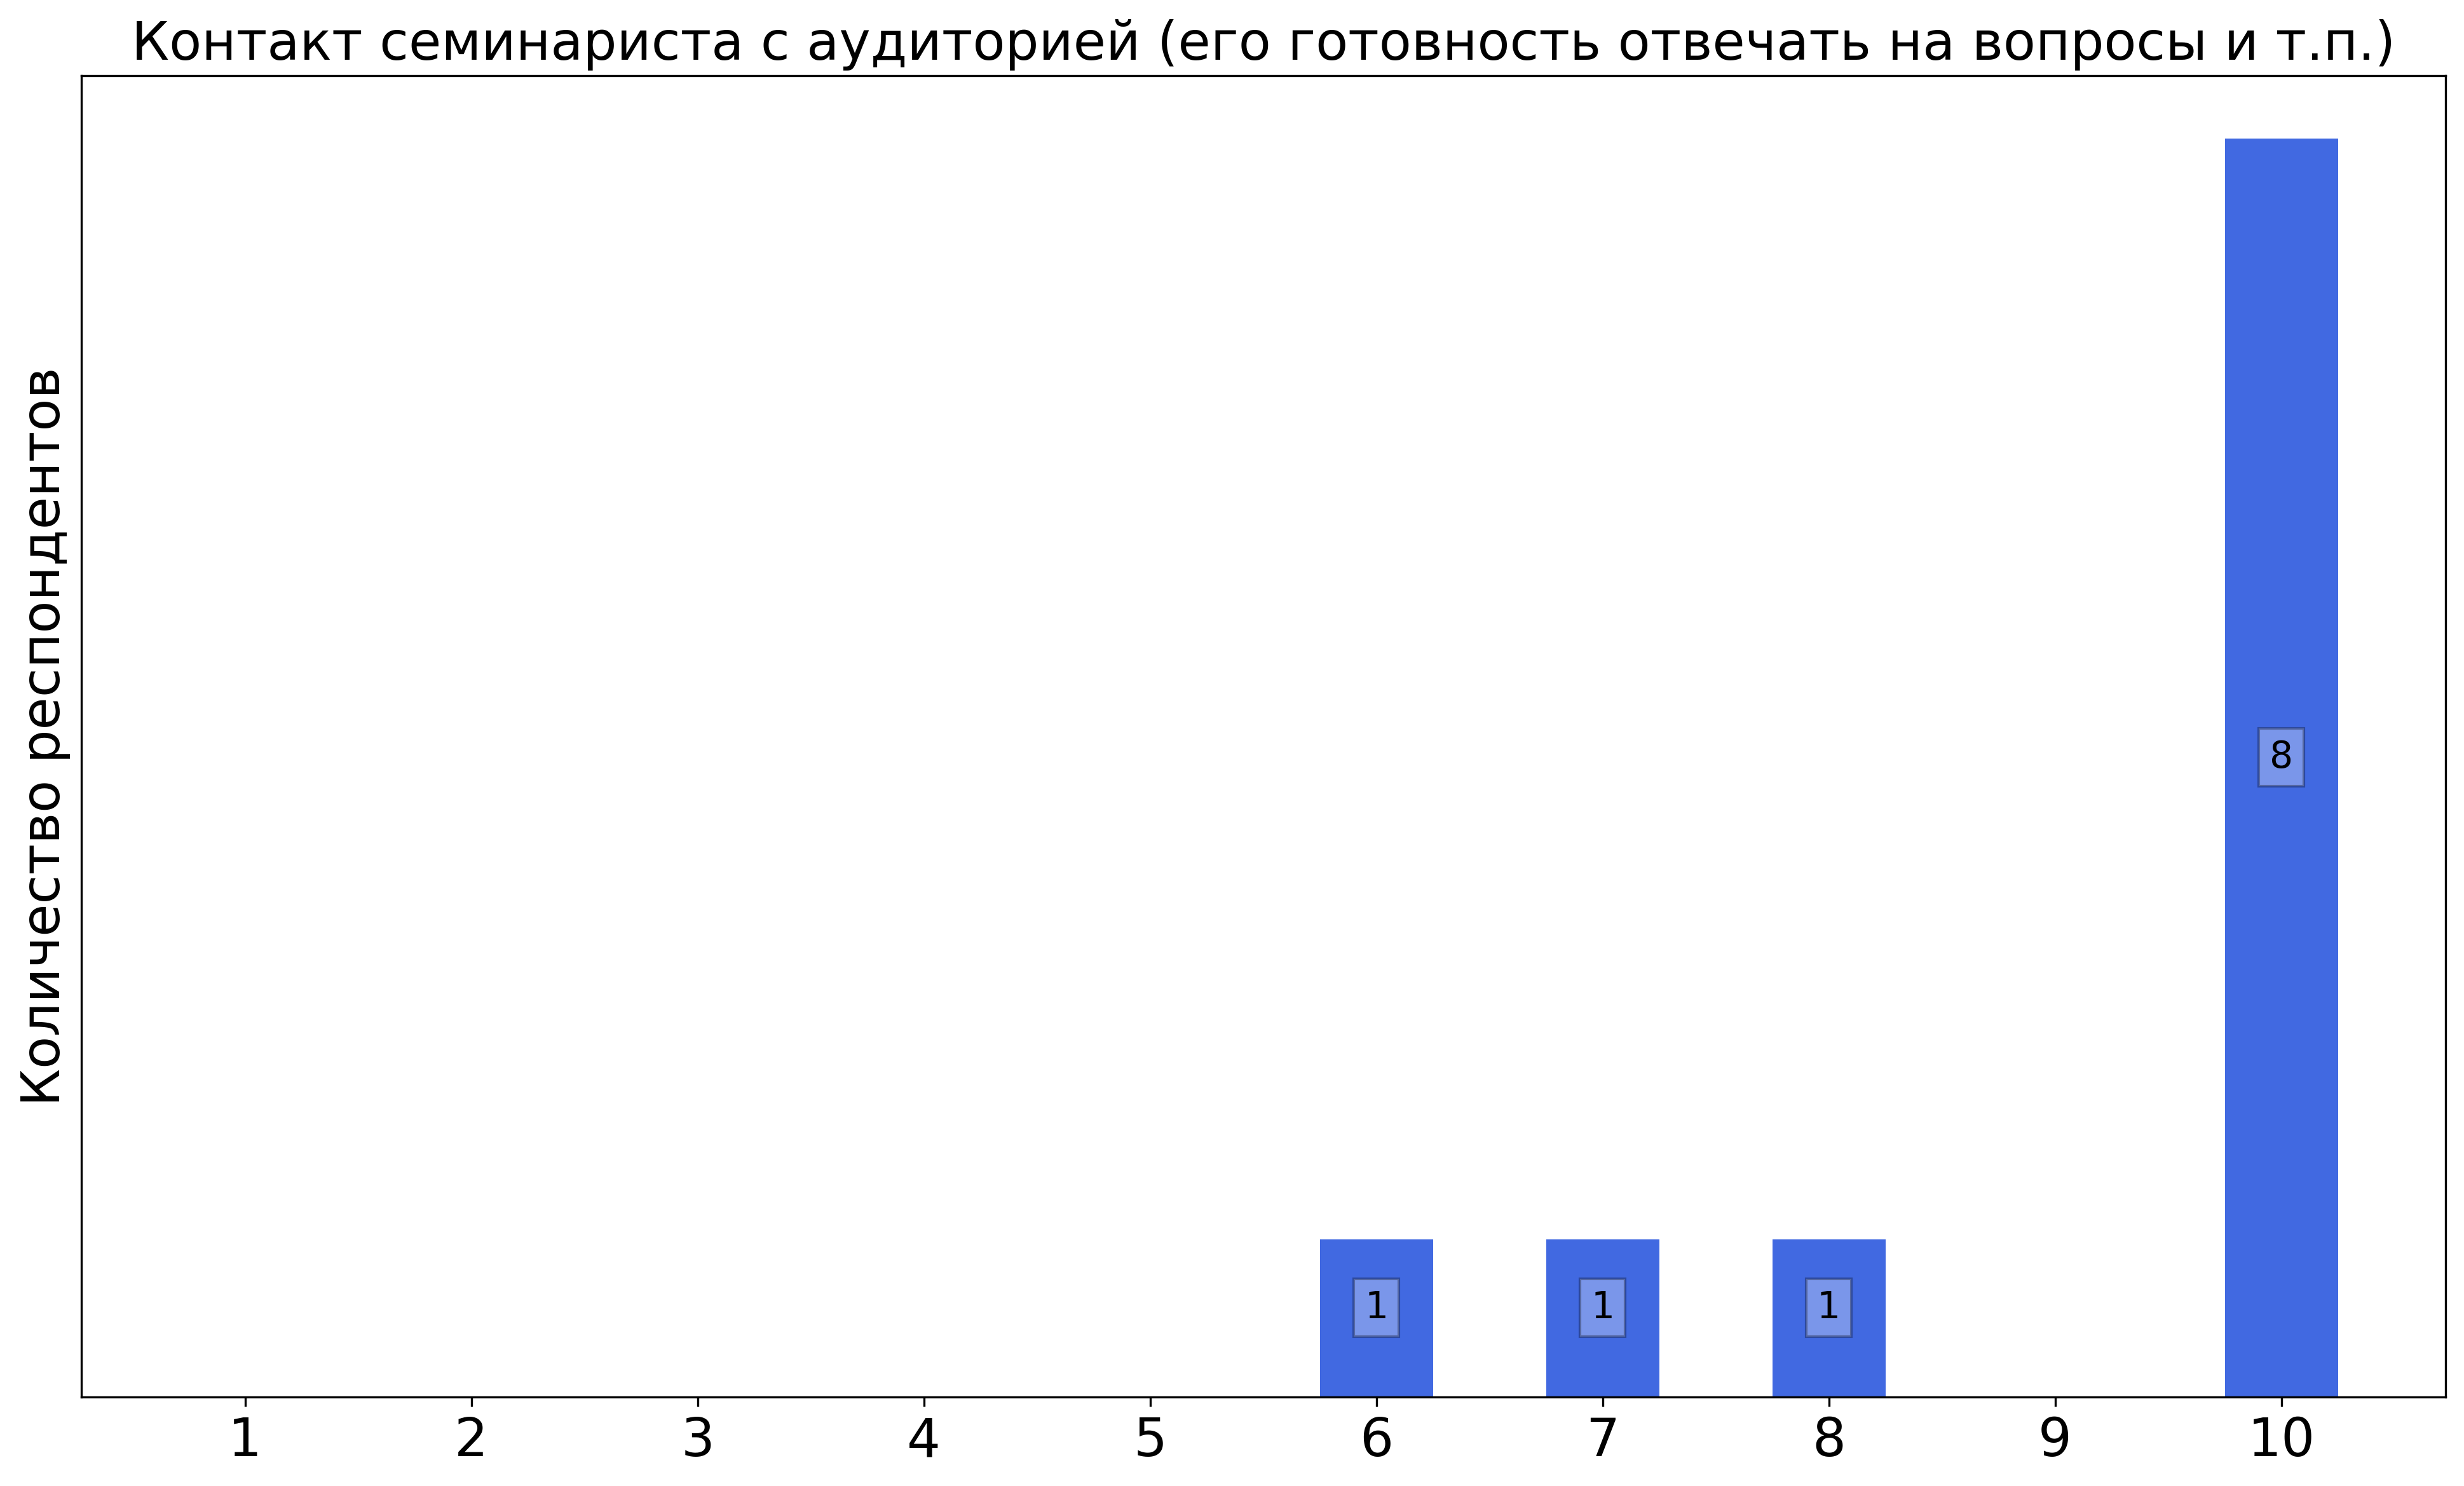
\includegraphics[width=\textwidth]{images/1 course/Дискретный анализ/seminarists-marks-Табунов А.В.-0.png}
            \end{subfigure}
            \begin{subfigure}[b]{0.45\textwidth}
                \centering
                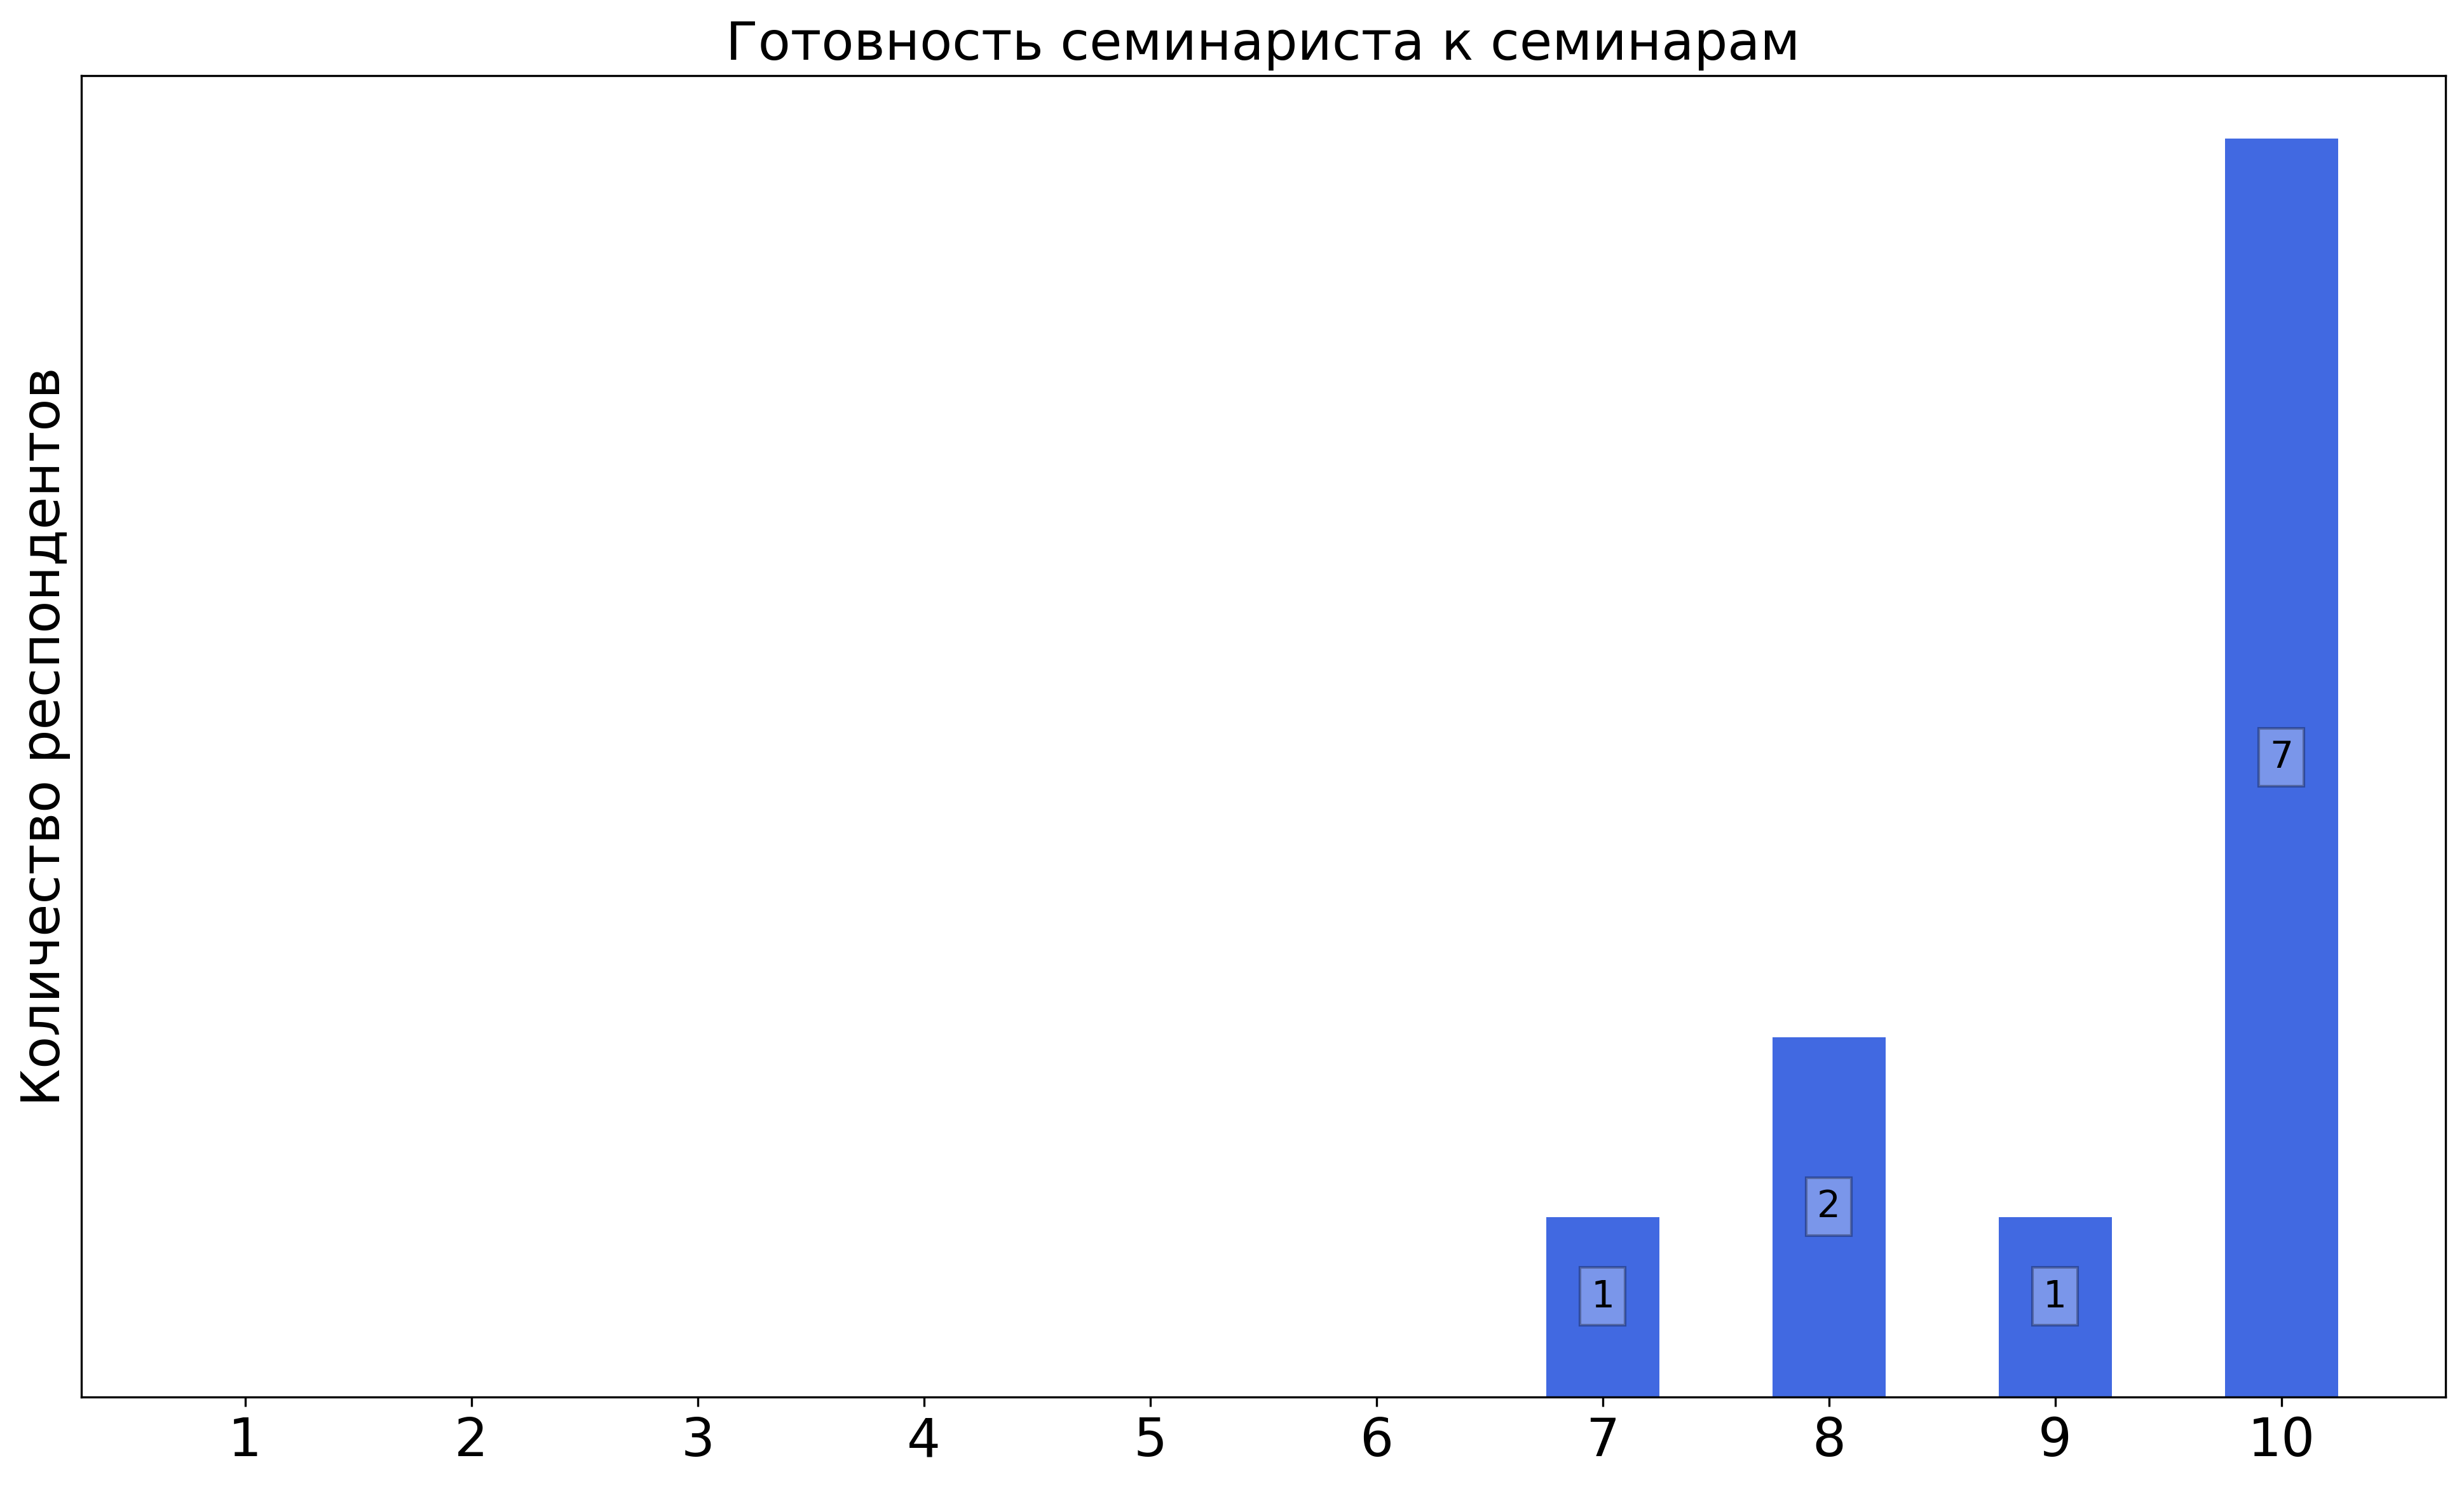
\includegraphics[width=\textwidth]{images/1 course/Дискретный анализ/seminarists-marks-Табунов А.В.-1.png}
            \end{subfigure}
            \begin{subfigure}[b]{0.45\textwidth}
                \centering
                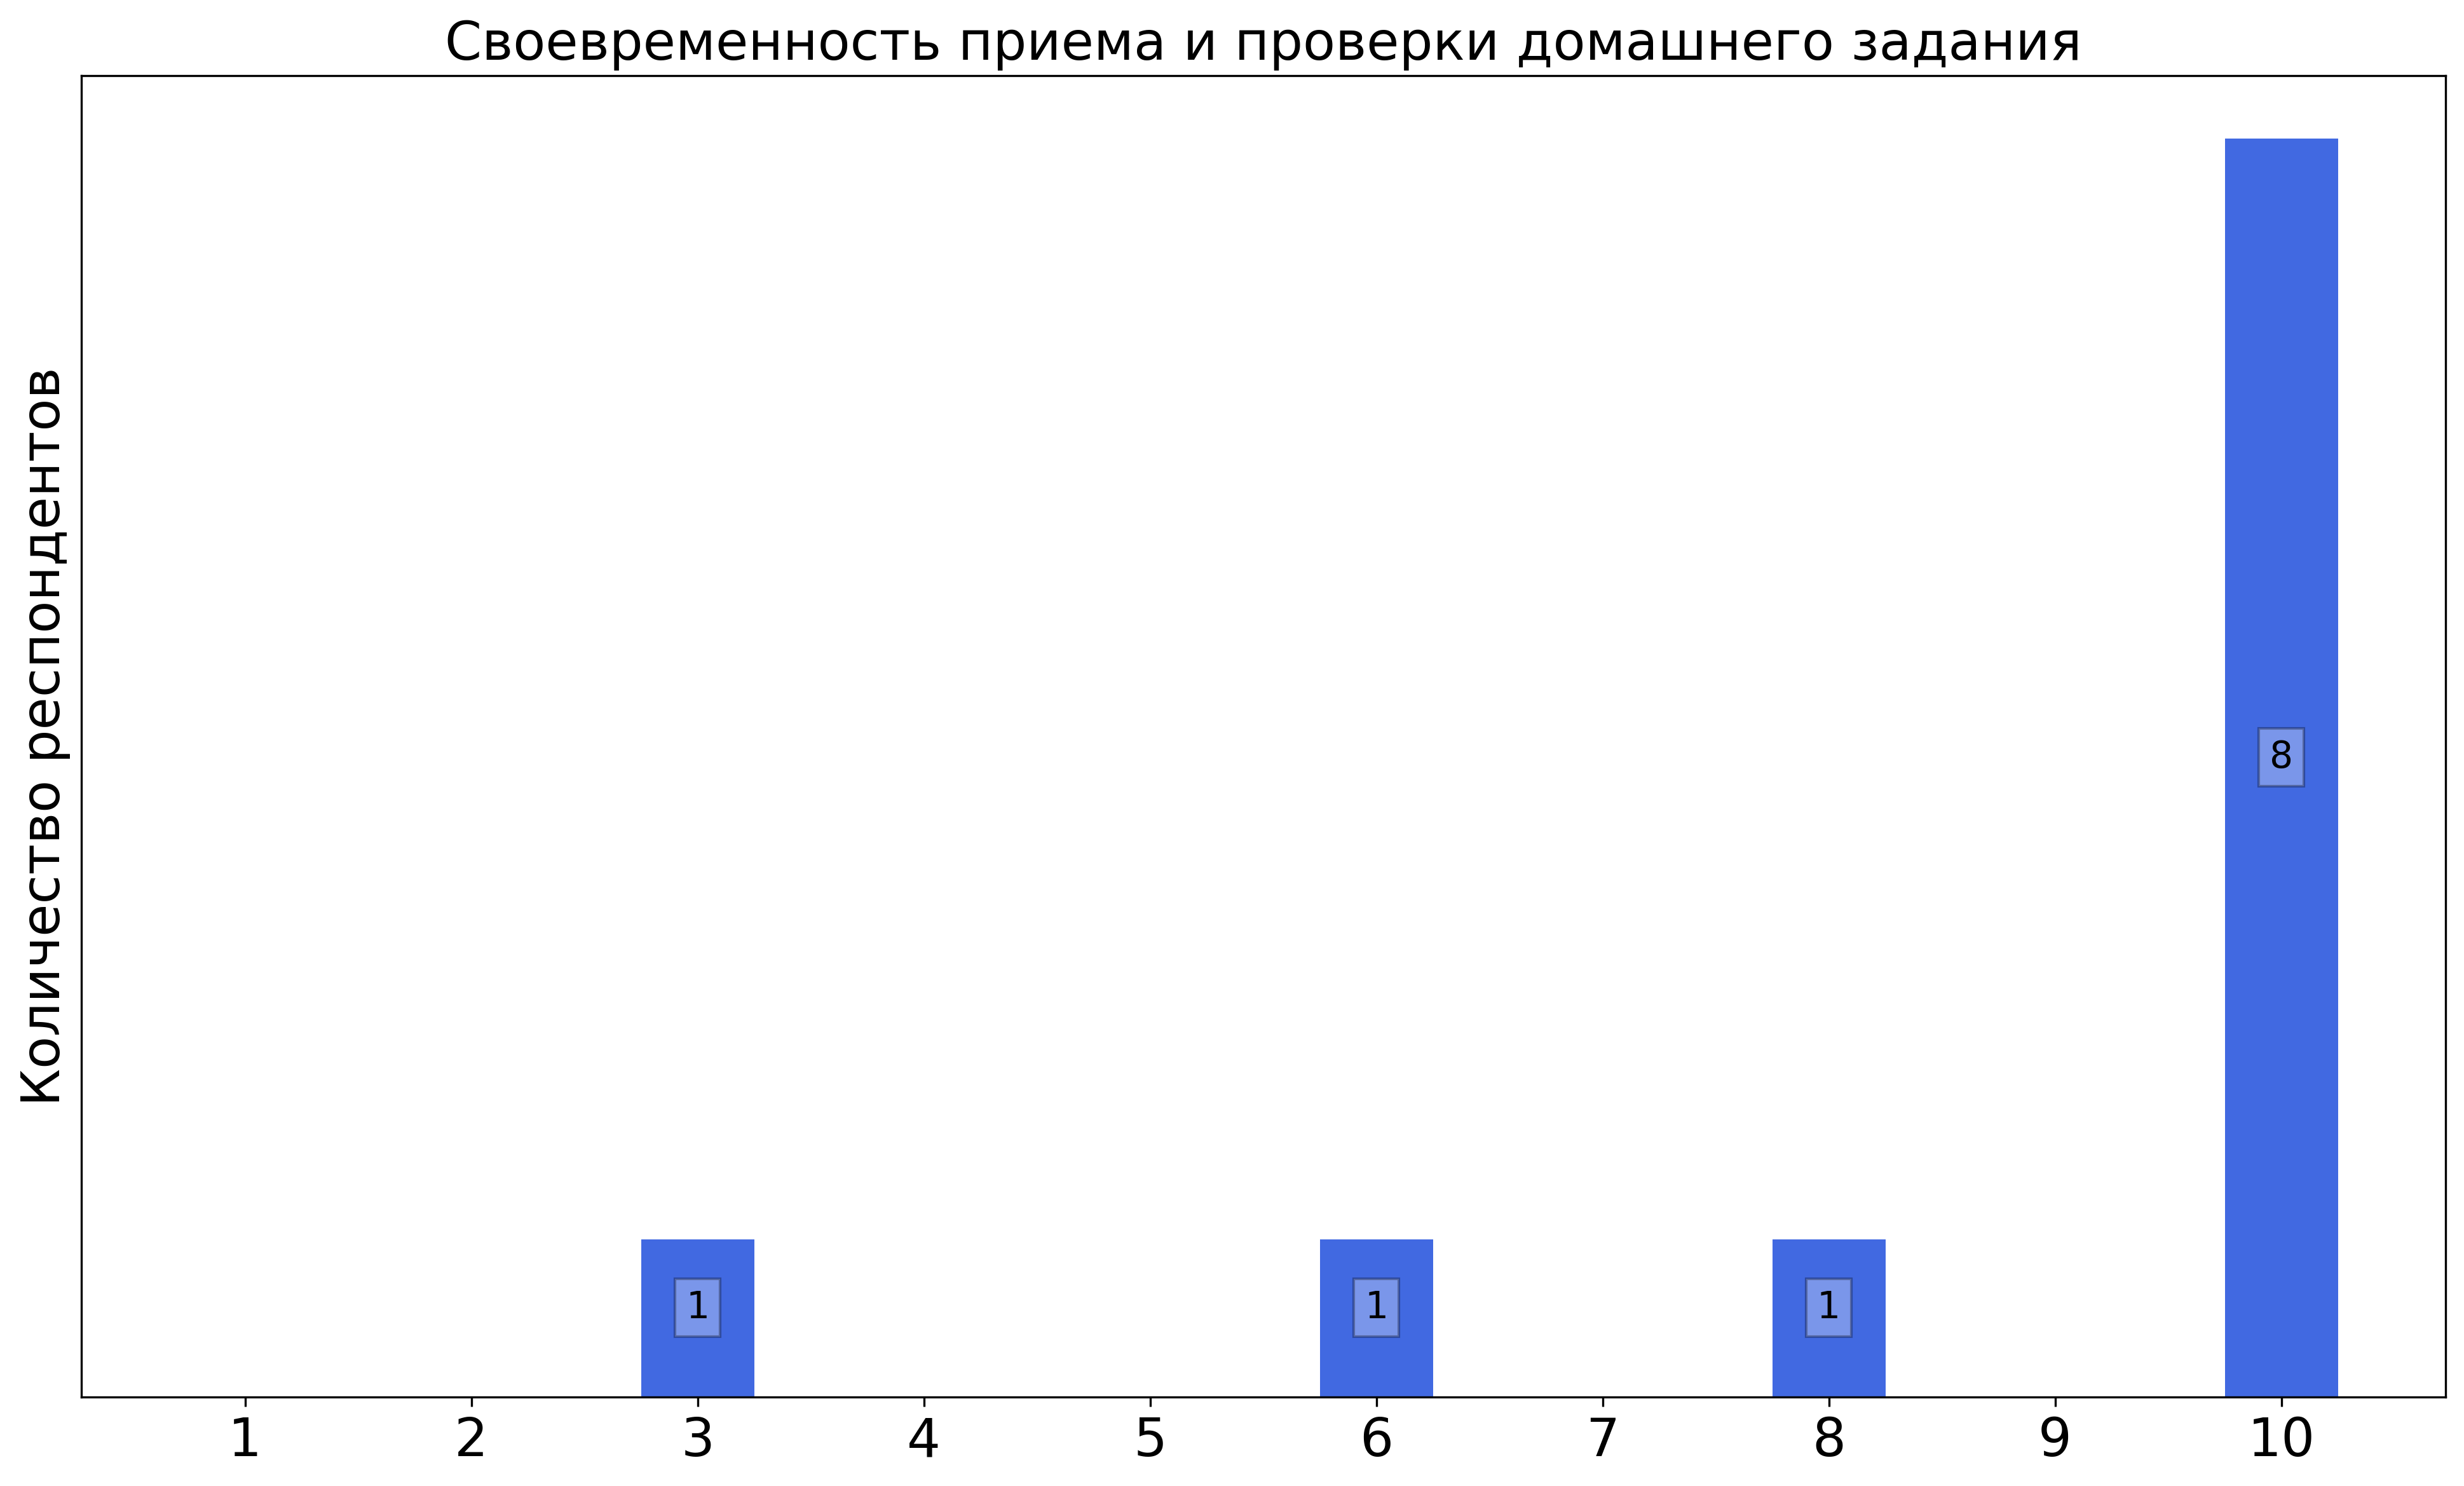
\includegraphics[width=\textwidth]{images/1 course/Дискретный анализ/seminarists-marks-Табунов А.В.-2.png}
            \end{subfigure}
            \begin{subfigure}[b]{0.45\textwidth}
                \centering
                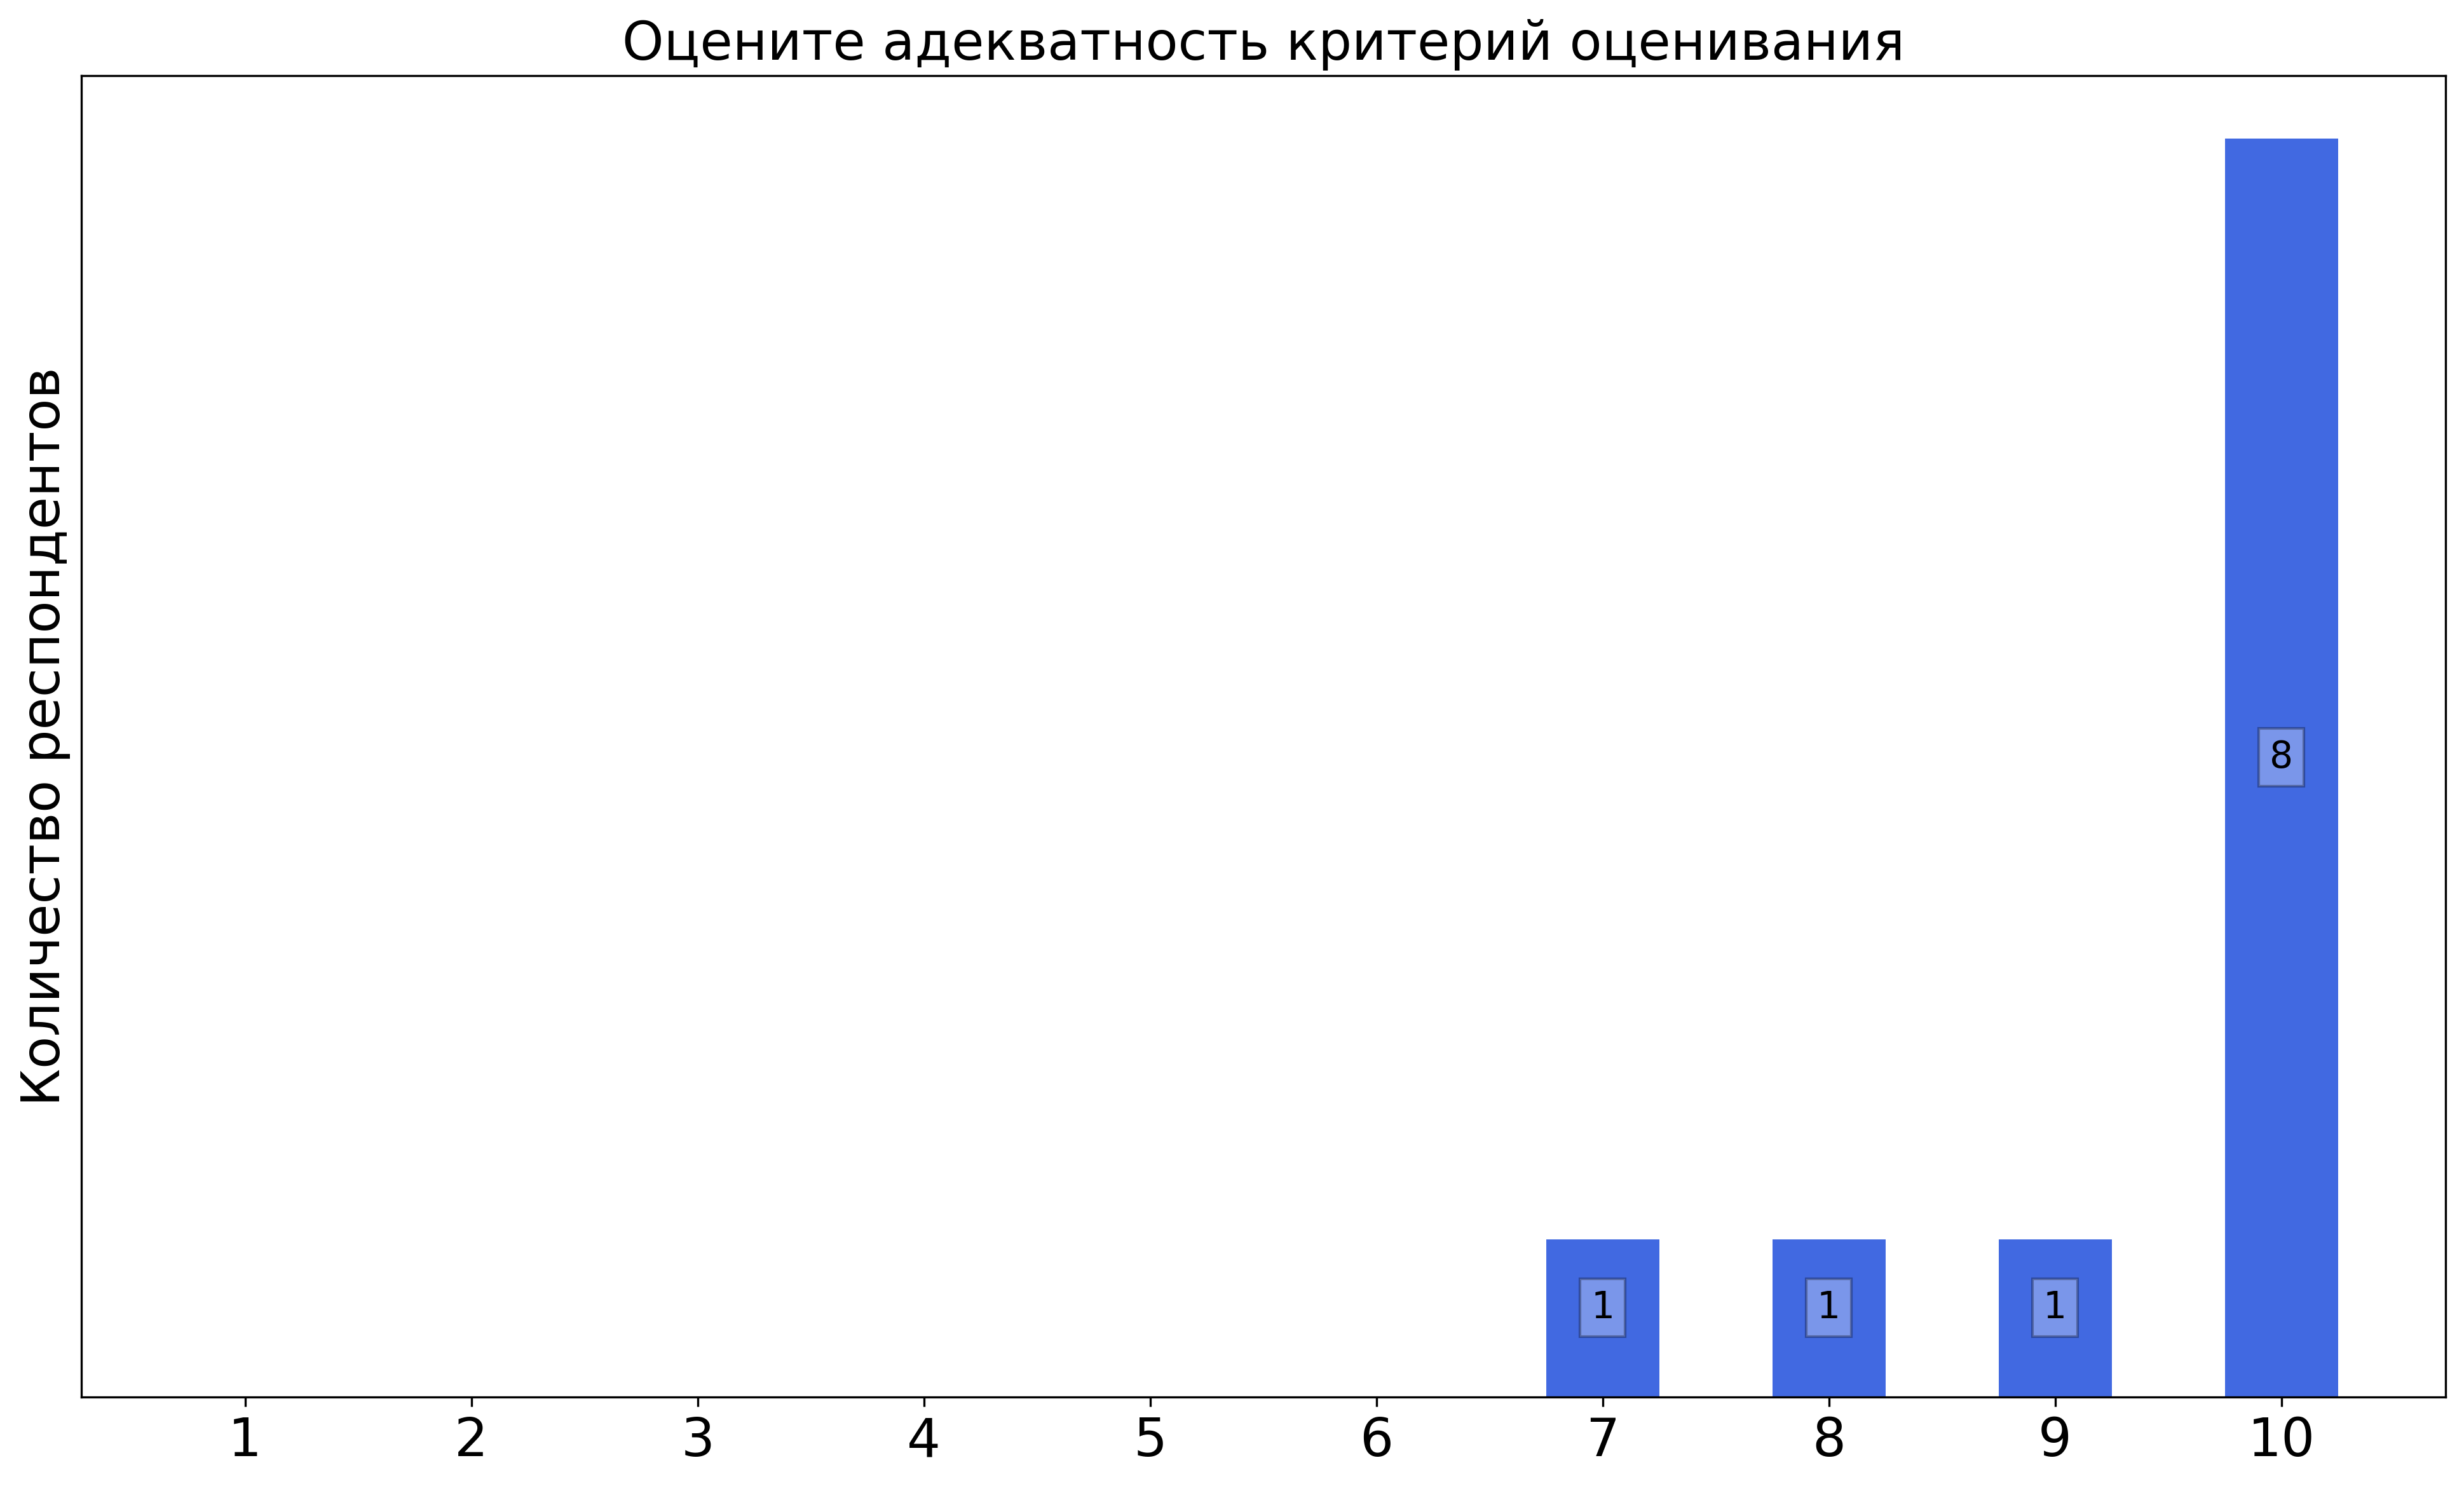
\includegraphics[width=\textwidth]{images/1 course/Дискретный анализ/seminarists-marks-Табунов А.В.-3.png}
            \end{subfigure}	
            \caption{Оценки респондентов о качестве преподавания семинаров}
        \end{figure}

        \textbf{Комментарии студентов о семинаристе\protect\footnote{сохранены оригинальные орфография и пунктуация}}
            \begin{commentbox} 
                Быстрый, но объясняет все непонятки. 
            \end{commentbox} 
        
            \begin{commentbox} 
                Очень понятно и постепенно всё излагает, буквально то, что нужно от данного курса. 
            \end{commentbox}


    \subsubsection{Отзыв студентов о семинарах. Семинарист: Теймуразов К.Б.}
		\begin{figure}[H]
			\centering
			\begin{subfigure}[b]{0.45\textwidth}
				\centering
				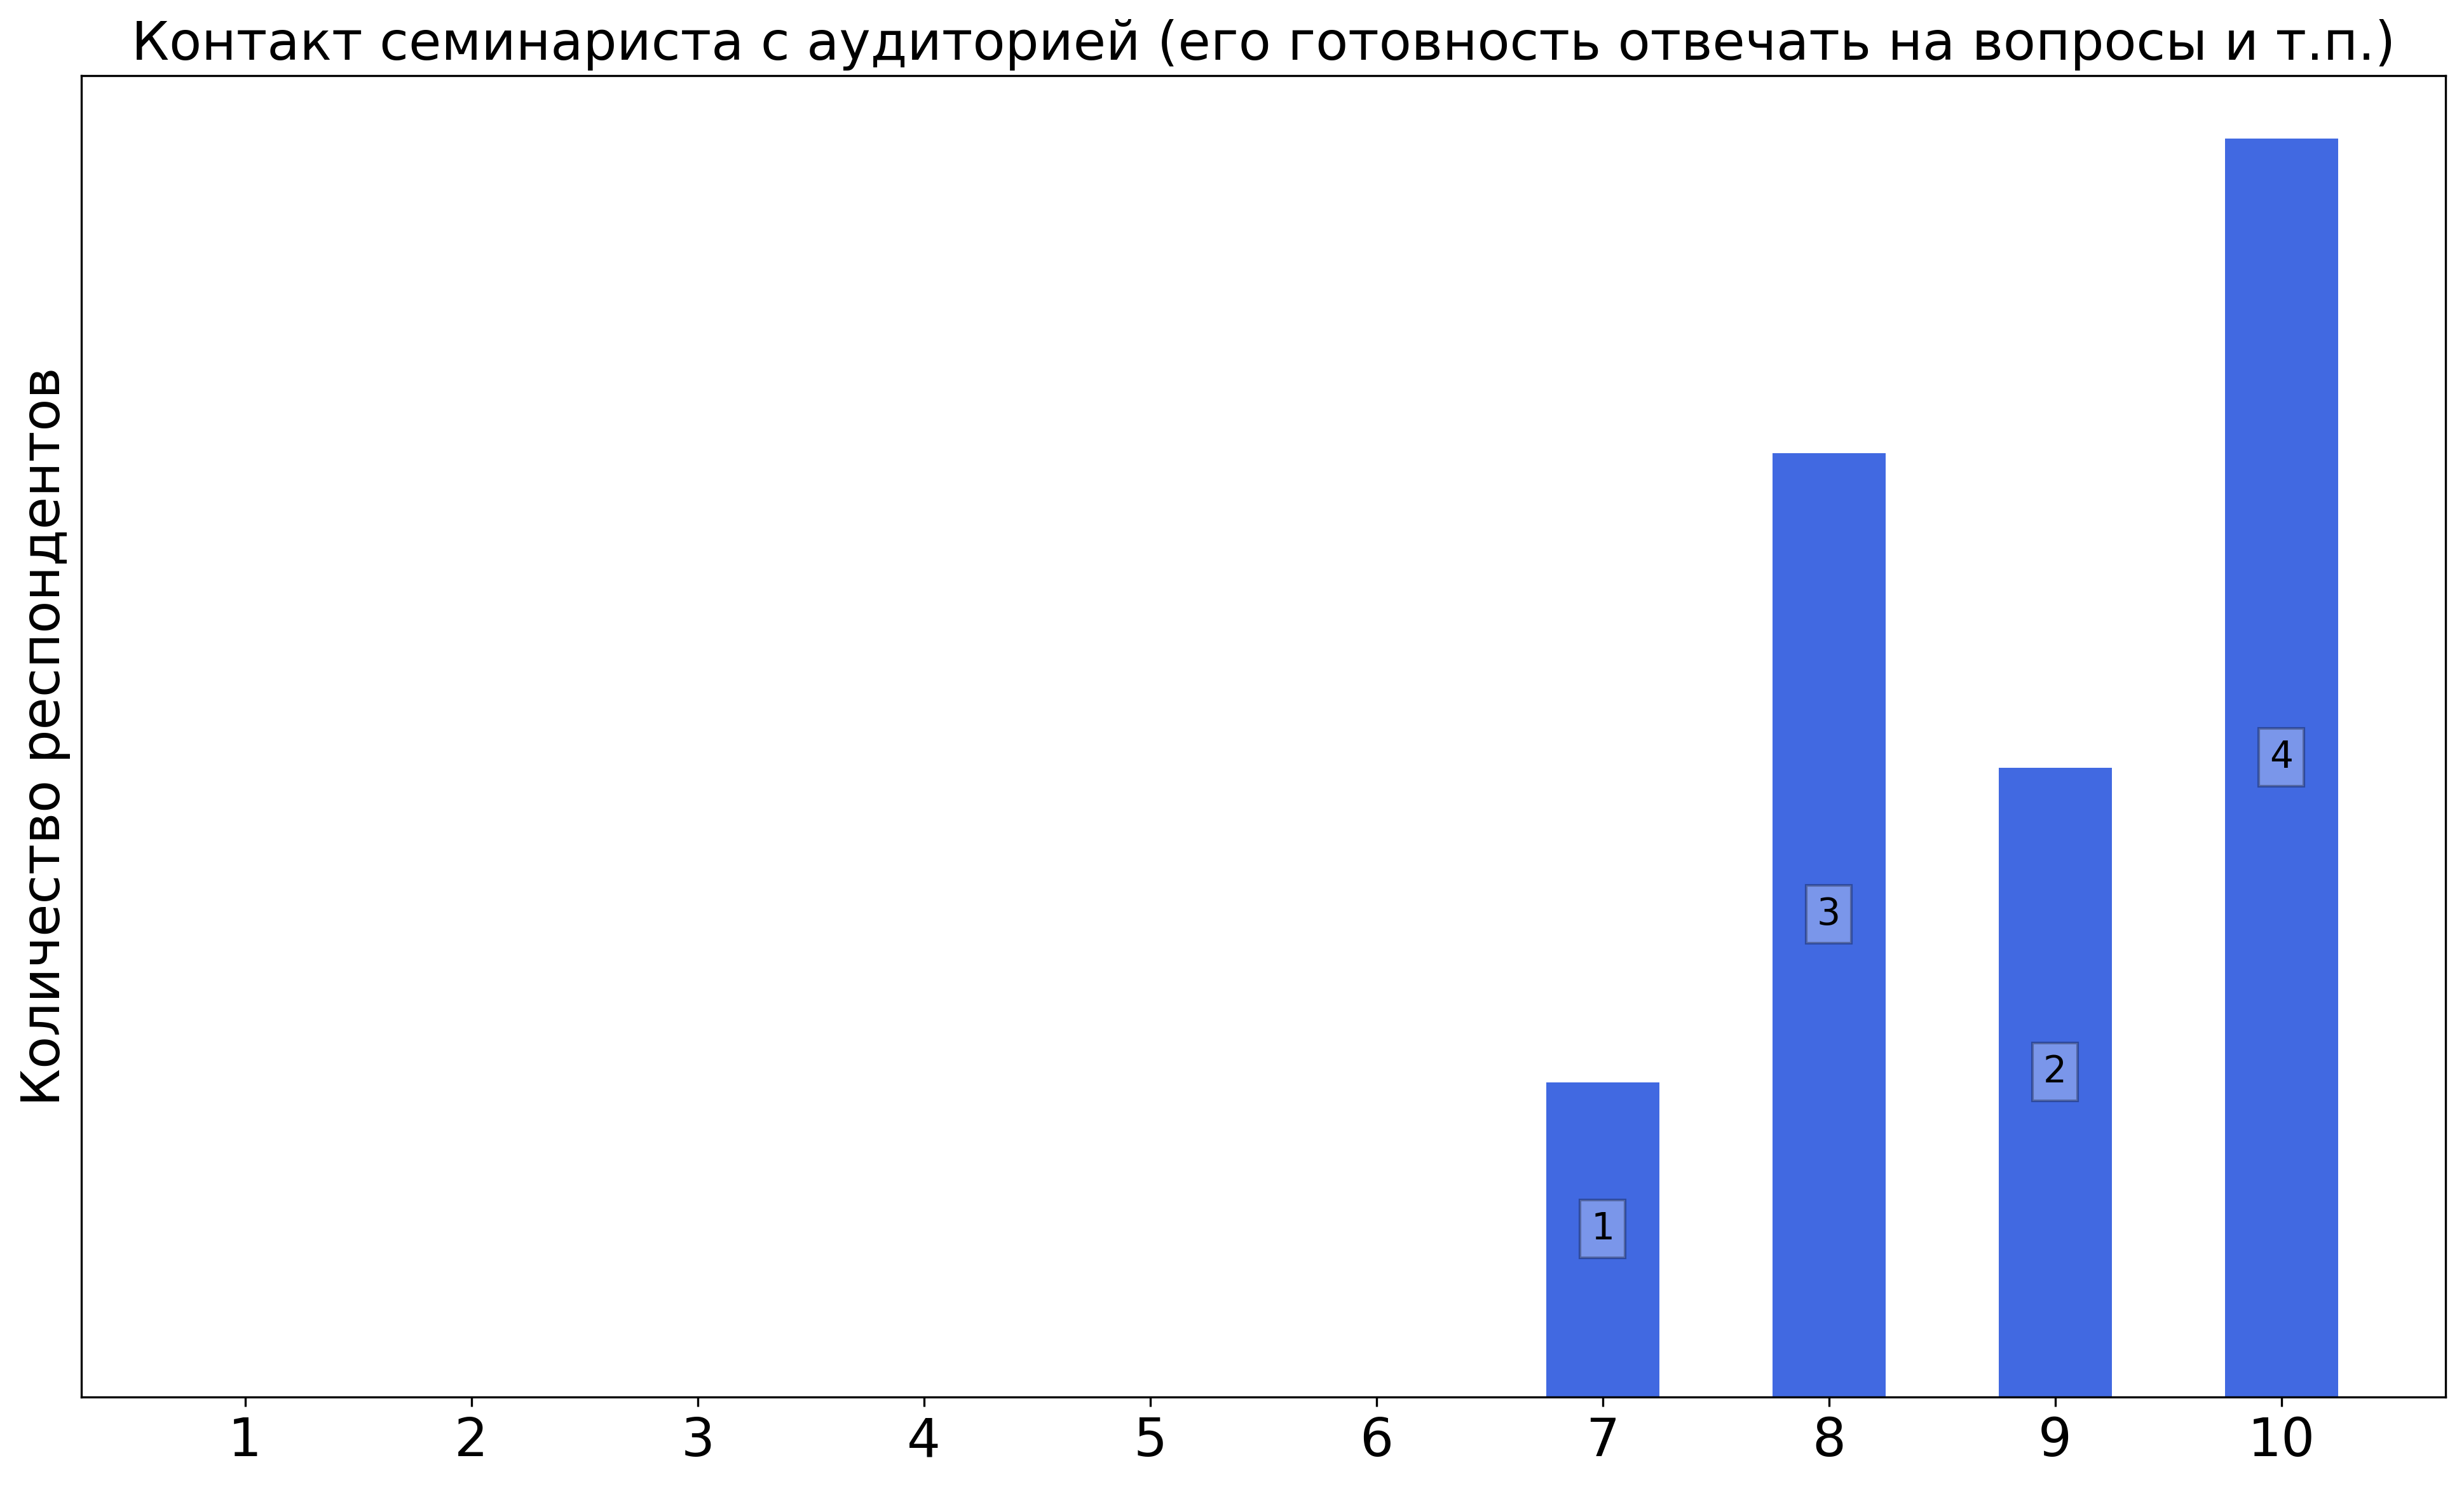
\includegraphics[width=\textwidth]{images/1 course/Дискретный анализ/seminarists-marks-Теймуразов К.Б.-0.png}
			\end{subfigure}
			\begin{subfigure}[b]{0.45\textwidth}
				\centering
				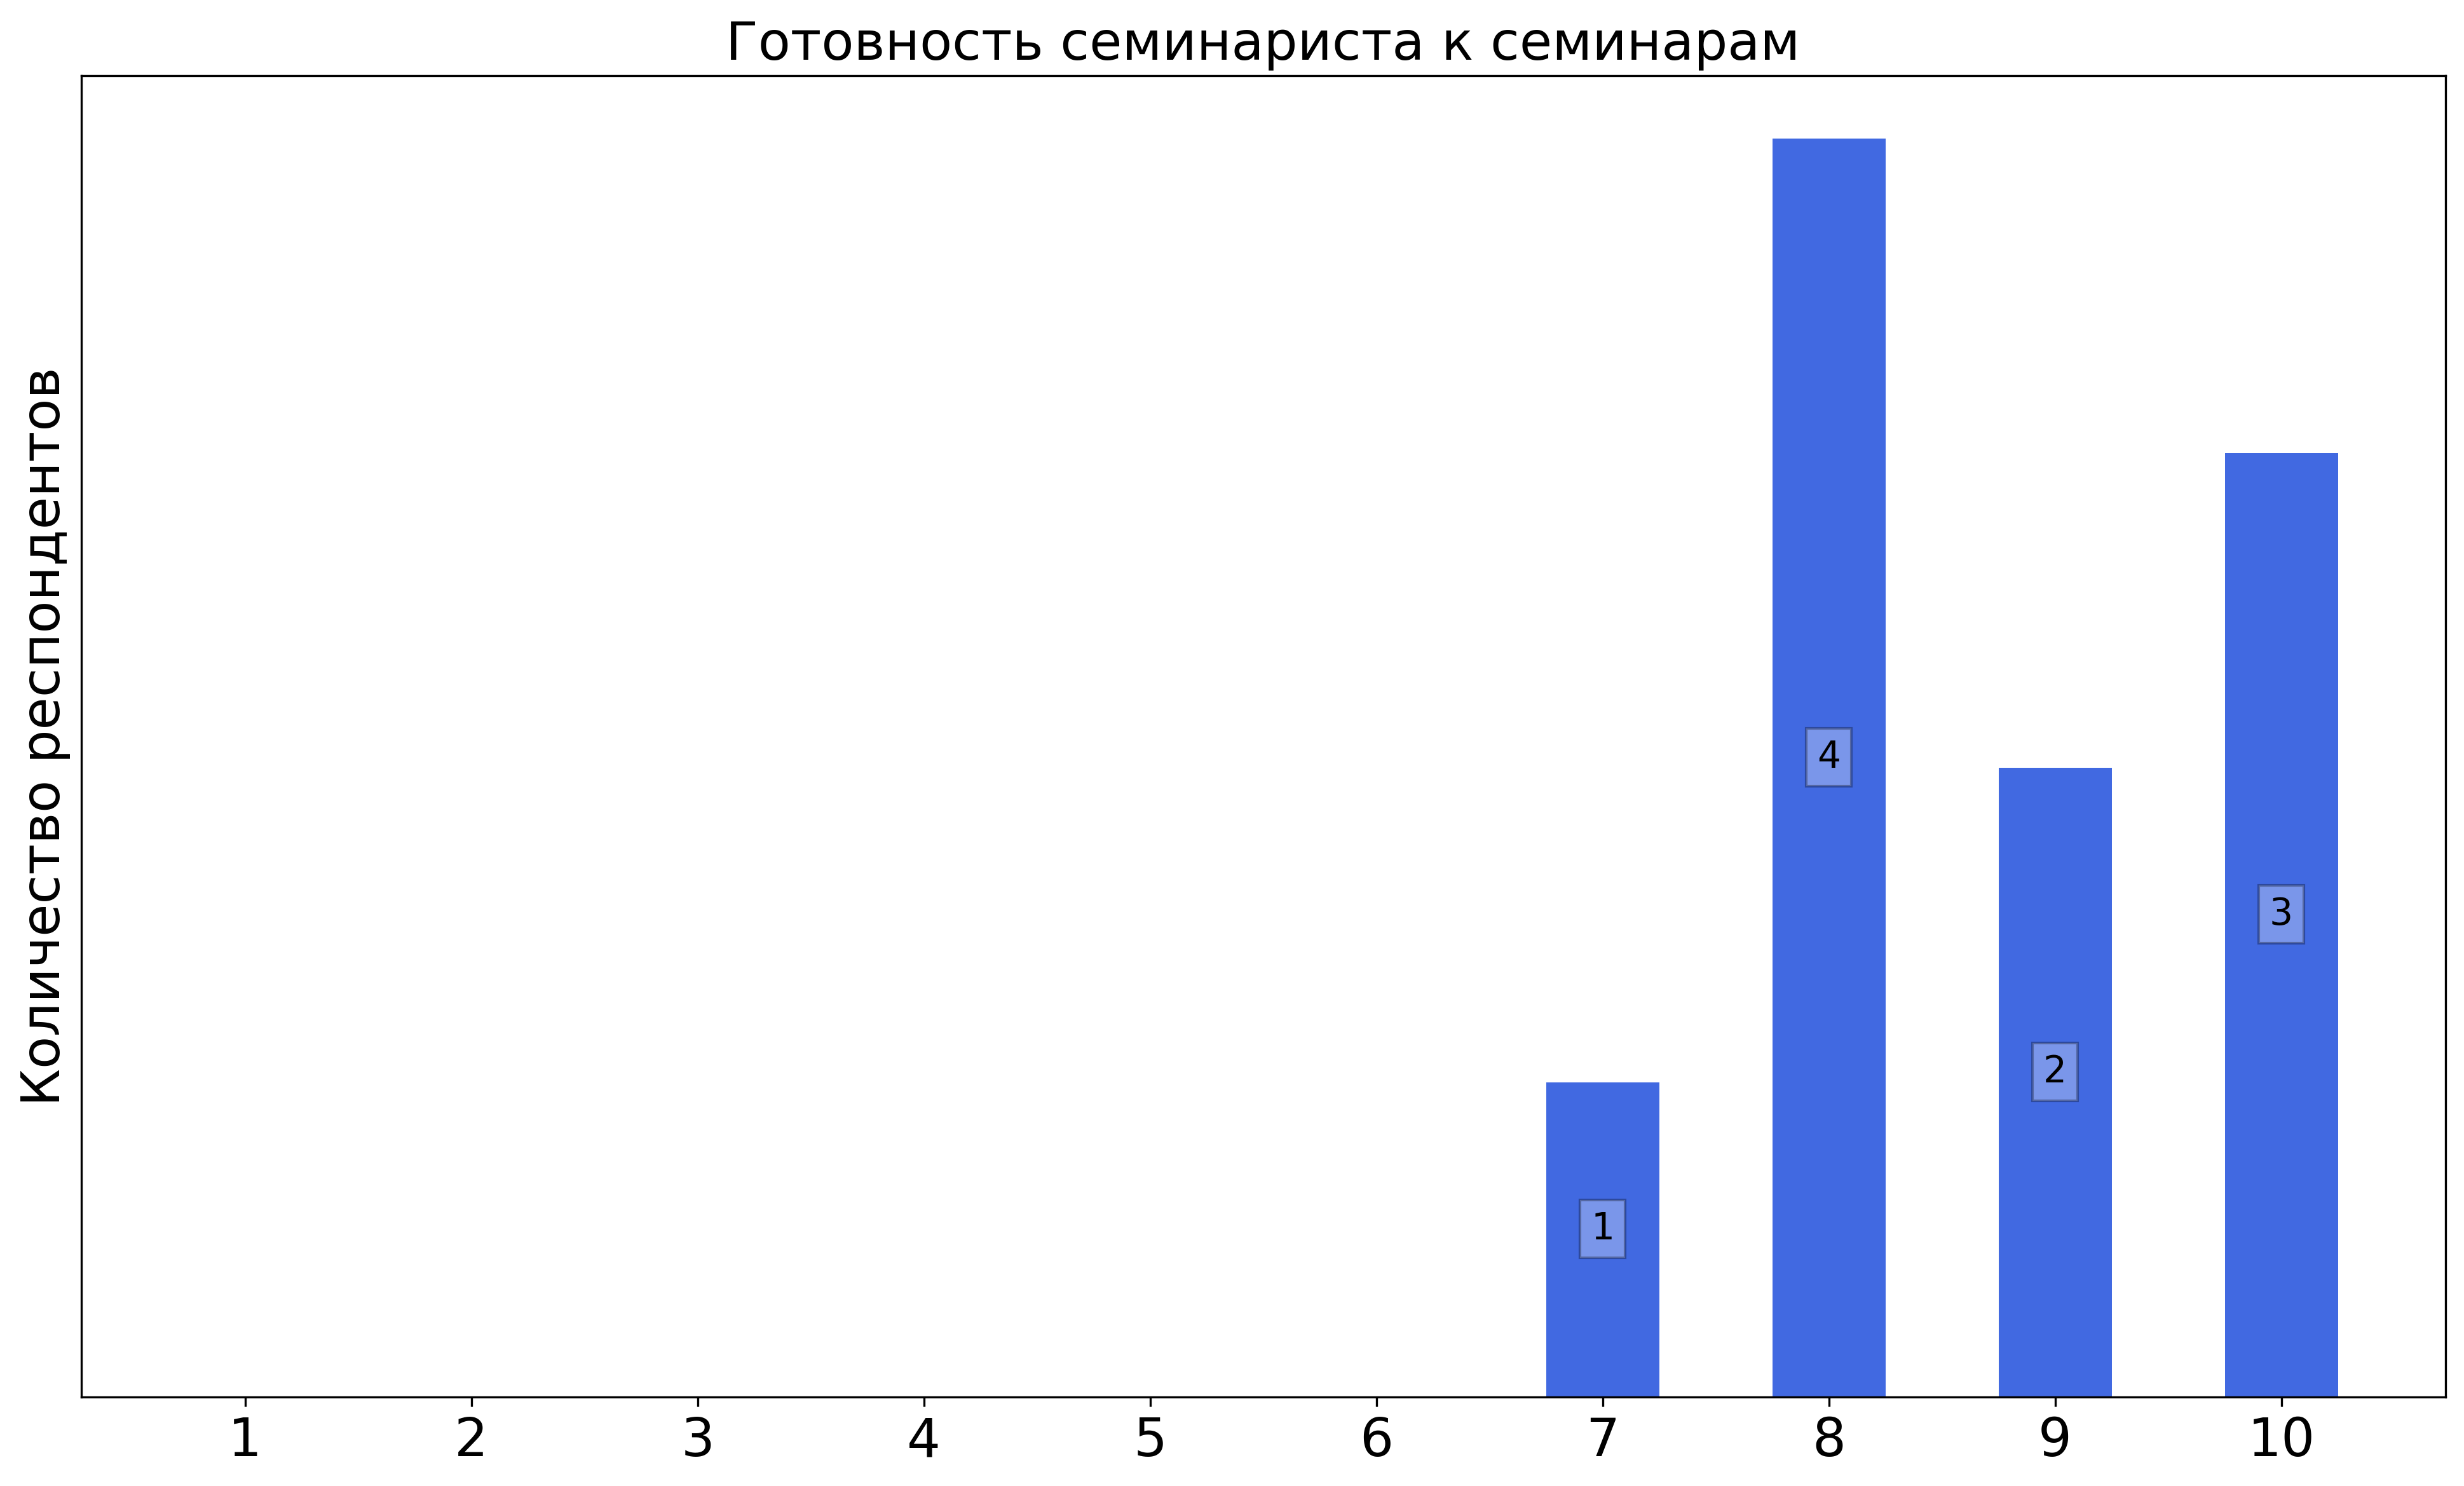
\includegraphics[width=\textwidth]{images/1 course/Дискретный анализ/seminarists-marks-Теймуразов К.Б.-1.png}
			\end{subfigure}
			\begin{subfigure}[b]{0.45\textwidth}
				\centering
				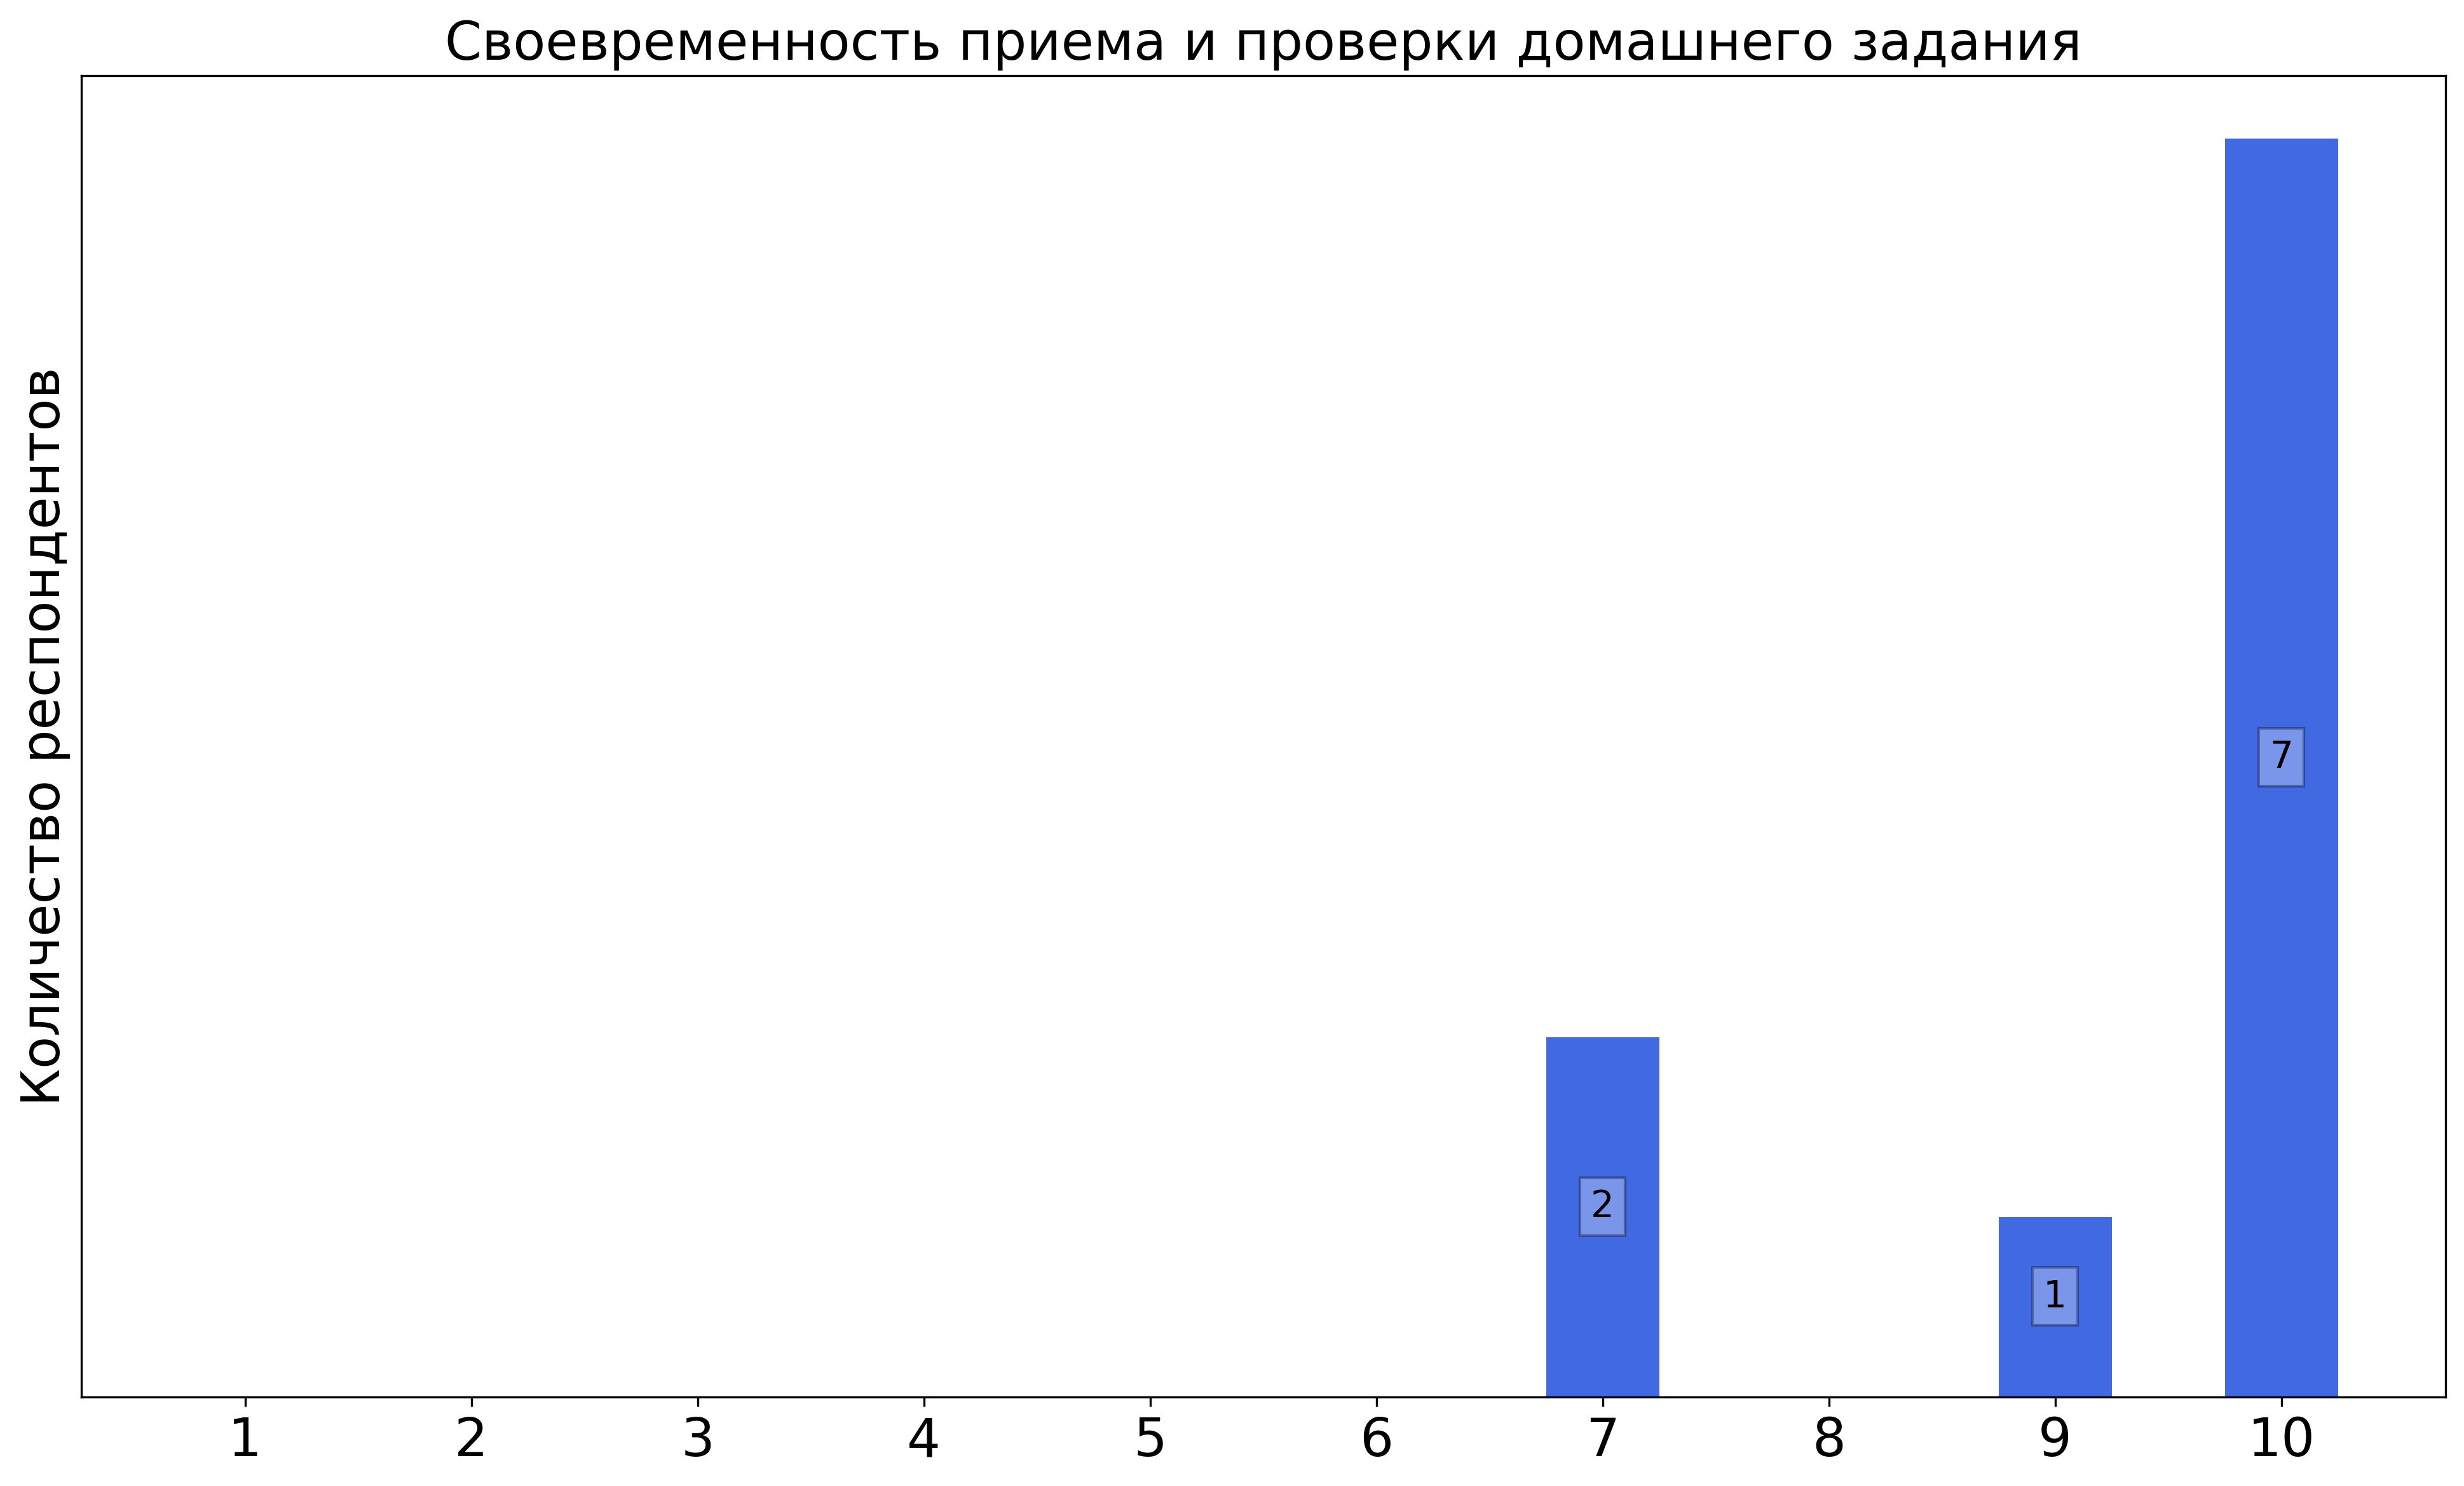
\includegraphics[width=\textwidth]{images/1 course/Дискретный анализ/seminarists-marks-Теймуразов К.Б.-2.png}
			\end{subfigure}
			\begin{subfigure}[b]{0.45\textwidth}
				\centering
				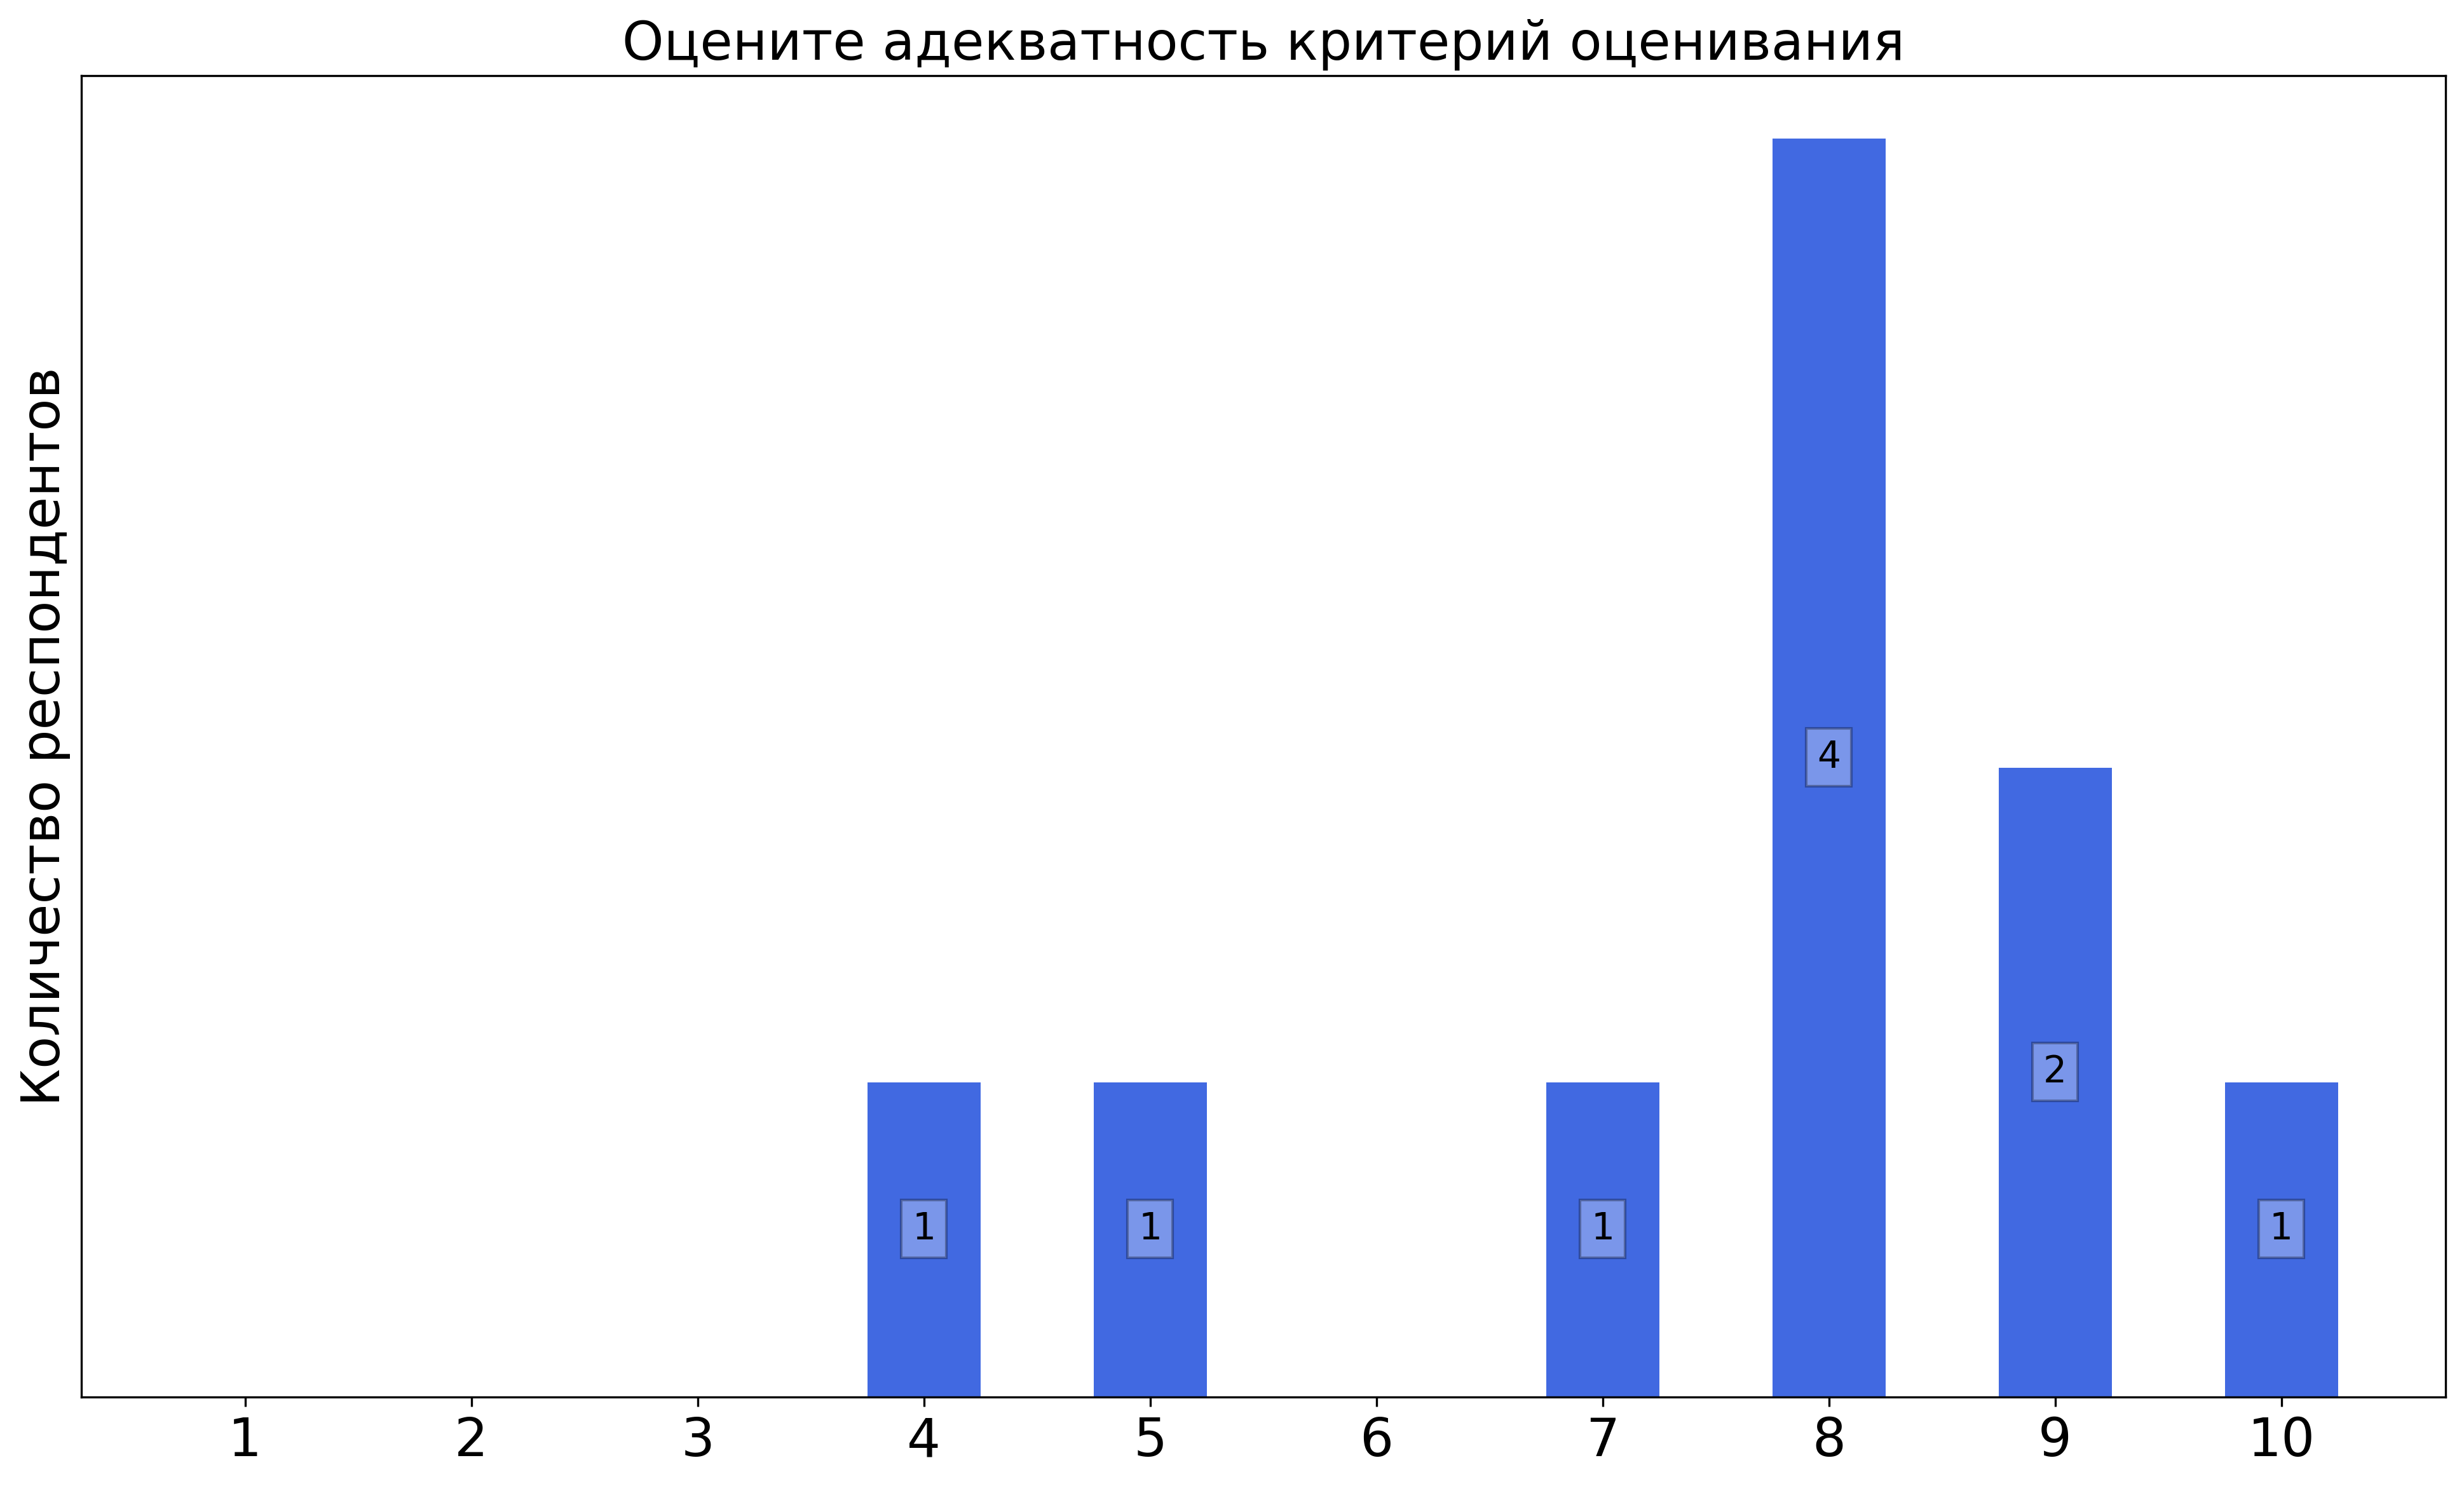
\includegraphics[width=\textwidth]{images/1 course/Дискретный анализ/seminarists-marks-Теймуразов К.Б.-3.png}
			\end{subfigure}	
			\caption{Оценки респондентов о качестве преподавания семинаров}
		\end{figure}

		\textbf{Комментарии студентов о семинаристе\protect\footnote{сохранены оригинальные орфография и пунктуация}}
            \begin{commentbox} 
                Неожиданно даёт контрольные. 
            \end{commentbox} 

    
    \subsubsection{Прочие комментарии и предложения по улучшению курса}
        \begin{commentbox}
            В целом курс интересный, однако преподаётся он так, как будто больше никогда не пригодится. 
        \end{commentbox}

        \begin{commentbox}
            По моему мнению дискретный анализ - предмет, которому в современном мире нет необходимости уделять столько времени. Мне кажется, что лучше было бы заменить его на изучение еще одного языка программирования
        \end{commentbox}

        \begin{commentbox}
            Хотелось бы, чтобы курс по дискретной математике имел больше отношения к программированию. Чтобы на нем разбирались алгоритмы, грамматики и тому подобное.
        \end{commentbox}

        \begin{commentbox}
            С такими лекциями очень бесполезным кажется
        \end{commentbox}

        \begin{commentbox}
            Вроде прикольно, жаль что не заботал
        \end{commentbox}